\documentclass[twoside]{book}

% Packages required by doxygen
\usepackage{calc}
\usepackage{doxygen}
\usepackage{graphicx}
\usepackage[utf8]{inputenc}
\usepackage{makeidx}
\usepackage{multicol}
\usepackage{multirow}
\usepackage{textcomp}
\usepackage[table]{xcolor}

% Font selection
\usepackage[T1]{fontenc}
\usepackage{mathptmx}
\usepackage[scaled=.90]{helvet}
\usepackage{courier}
\usepackage{amssymb}
\usepackage{sectsty}
\renewcommand{\familydefault}{\sfdefault}
\allsectionsfont{%
  \fontseries{bc}\selectfont%
  \color{darkgray}%
}
\renewcommand{\DoxyLabelFont}{%
  \fontseries{bc}\selectfont%
  \color{darkgray}%
}

% Page & text layout
\usepackage{geometry}
\geometry{%
  a4paper,%
  top=2.5cm,%
  bottom=2.5cm,%
  left=2.5cm,%
  right=2.5cm%
}
\tolerance=750
\hfuzz=15pt
\hbadness=750
\setlength{\emergencystretch}{15pt}
\setlength{\parindent}{0cm}
\setlength{\parskip}{0.2cm}
\makeatletter
\renewcommand{\paragraph}{%
  \@startsection{paragraph}{4}{0ex}{-1.0ex}{1.0ex}{%
    \normalfont\normalsize\bfseries\SS@parafont%
  }%
}
\renewcommand{\subparagraph}{%
  \@startsection{subparagraph}{5}{0ex}{-1.0ex}{1.0ex}{%
    \normalfont\normalsize\bfseries\SS@subparafont%
  }%
}
\makeatother

% Headers & footers
\usepackage{fancyhdr}
\pagestyle{fancyplain}
\fancyhead[LE]{\fancyplain{}{\bfseries\thepage}}
\fancyhead[CE]{\fancyplain{}{}}
\fancyhead[RE]{\fancyplain{}{\bfseries\leftmark}}
\fancyhead[LO]{\fancyplain{}{\bfseries\rightmark}}
\fancyhead[CO]{\fancyplain{}{}}
\fancyhead[RO]{\fancyplain{}{\bfseries\thepage}}
\fancyfoot[LE]{\fancyplain{}{}}
\fancyfoot[CE]{\fancyplain{}{}}
\fancyfoot[RE]{\fancyplain{}{\bfseries\scriptsize Generated on Tue Feb 25 2014 04\-:32\-:18 for Covert Collisions by Doxygen }}
\fancyfoot[LO]{\fancyplain{}{\bfseries\scriptsize Generated on Tue Feb 25 2014 04\-:32\-:18 for Covert Collisions by Doxygen }}
\fancyfoot[CO]{\fancyplain{}{}}
\fancyfoot[RO]{\fancyplain{}{}}
\renewcommand{\footrulewidth}{0.4pt}
\renewcommand{\chaptermark}[1]{%
  \markboth{#1}{}%
}
\renewcommand{\sectionmark}[1]{%
  \markright{\thesection\ #1}%
}

% Indices & bibliography
\usepackage{natbib}
\usepackage[titles]{tocloft}
\setcounter{tocdepth}{3}
\setcounter{secnumdepth}{5}
\makeindex

% Hyperlinks (required, but should be loaded last)
\usepackage{ifpdf}
\ifpdf
  \usepackage[pdftex,pagebackref=true]{hyperref}
\else
  \usepackage[ps2pdf,pagebackref=true]{hyperref}
\fi
\hypersetup{%
  colorlinks=true,%
  linkcolor=blue,%
  citecolor=blue,%
  unicode%
}

% Custom commands
\newcommand{\clearemptydoublepage}{%
  \newpage{\pagestyle{empty}\cleardoublepage}%
}


%===== C O N T E N T S =====

\begin{document}

% Titlepage & ToC
\hypersetup{pageanchor=false}
\pagenumbering{roman}
\begin{titlepage}
\vspace*{7cm}
\begin{center}%
{\Large Covert Collisions }\\
\vspace*{1cm}
{\large Generated by Doxygen 1.8.5}\\
\vspace*{0.5cm}
{\small Tue Feb 25 2014 04:32:18}\\
\end{center}
\end{titlepage}
\clearemptydoublepage
\tableofcontents
\clearemptydoublepage
\pagenumbering{arabic}
\hypersetup{pageanchor=true}

%--- Begin generated contents ---
\chapter{Hierarchical Index}
\section{Class Hierarchy}
This inheritance list is sorted roughly, but not completely, alphabetically\-:\begin{DoxyCompactList}
\item \contentsline{section}{A\-Renderable}{\pageref{classARenderable}}{}
\begin{DoxyCompactList}
\item \contentsline{section}{C\-Player}{\pageref{classCPlayer}}{}
\item \contentsline{section}{C\-Tile}{\pageref{classCTile}}{}
\end{DoxyCompactList}
\item \contentsline{section}{A\-User\-Input}{\pageref{classAUserInput}}{}
\begin{DoxyCompactList}
\item \contentsline{section}{C\-Player}{\pageref{classCPlayer}}{}
\item \contentsline{section}{C\-U\-I}{\pageref{classCUI}}{}
\end{DoxyCompactList}
\item \contentsline{section}{C\-Game}{\pageref{classCGame}}{}
\item \contentsline{section}{C\-Render\-Engine}{\pageref{classCRenderEngine}}{}
\item \contentsline{section}{D\-Physics}{\pageref{classDPhysics}}{}
\begin{DoxyCompactList}
\item \contentsline{section}{C\-Player}{\pageref{classCPlayer}}{}
\end{DoxyCompactList}
\item \contentsline{section}{I\-Get\-Collision\-Data}{\pageref{classIGetCollisionData}}{}
\begin{DoxyCompactList}
\item \contentsline{section}{C\-Tile\-\_\-\-Container}{\pageref{classCTile__Container}}{}
\end{DoxyCompactList}
\item \contentsline{section}{I\-Get\-Render\-Data}{\pageref{classIGetRenderData}}{}
\begin{DoxyCompactList}
\item \contentsline{section}{C\-Tile\-\_\-\-Container}{\pageref{classCTile__Container}}{}
\end{DoxyCompactList}
\item \contentsline{section}{I\-Updateable}{\pageref{classIUpdateable}}{}
\begin{DoxyCompactList}
\item \contentsline{section}{A\-Update}{\pageref{classAUpdate}}{}
\begin{DoxyCompactList}
\item \contentsline{section}{C\-Player}{\pageref{classCPlayer}}{}
\item \contentsline{section}{C\-Tile}{\pageref{classCTile}}{}
\end{DoxyCompactList}
\item \contentsline{section}{C\-Physics\-Engine}{\pageref{classCPhysicsEngine}}{}
\item \contentsline{section}{C\-Tile\-\_\-\-Container}{\pageref{classCTile__Container}}{}
\item \contentsline{section}{C\-U\-I}{\pageref{classCUI}}{}
\end{DoxyCompactList}
\item \contentsline{section}{A\-User\-Input\-:\-:S\-Key\-States}{\pageref{structAUserInput_1_1SKeyStates}}{}
\item \contentsline{section}{D\-Physics\-:\-:S\-Physics}{\pageref{structDPhysics_1_1SPhysics}}{}
\item Sprite\begin{DoxyCompactList}
\item \contentsline{section}{C\-Sprite}{\pageref{classCSprite}}{}
\end{DoxyCompactList}
\item Texture\begin{DoxyCompactList}
\item \contentsline{section}{C\-Texture}{\pageref{classCTexture}}{}
\end{DoxyCompactList}
\end{DoxyCompactList}

\chapter{Class Index}
\section{Class List}
Here are the classes, structs, unions and interfaces with brief descriptions\-:\begin{DoxyCompactList}
\item\contentsline{section}{\hyperlink{classARenderable}{A\-Renderable} }{\pageref{classARenderable}}{}
\item\contentsline{section}{\hyperlink{classAUpdate}{A\-Update} }{\pageref{classAUpdate}}{}
\item\contentsline{section}{\hyperlink{classAUserInput}{A\-User\-Input} }{\pageref{classAUserInput}}{}
\item\contentsline{section}{\hyperlink{classCGame}{C\-Game} }{\pageref{classCGame}}{}
\item\contentsline{section}{\hyperlink{classCPlayer}{C\-Player} }{\pageref{classCPlayer}}{}
\item\contentsline{section}{\hyperlink{classCRenderEngine}{C\-Render\-Engine} }{\pageref{classCRenderEngine}}{}
\item\contentsline{section}{\hyperlink{classCSprite}{C\-Sprite} }{\pageref{classCSprite}}{}
\item\contentsline{section}{\hyperlink{classCTexture}{C\-Texture} }{\pageref{classCTexture}}{}
\item\contentsline{section}{\hyperlink{classCTile}{C\-Tile} }{\pageref{classCTile}}{}
\item\contentsline{section}{\hyperlink{classCTile__Container}{C\-Tile\-\_\-\-Container} }{\pageref{classCTile__Container}}{}
\item\contentsline{section}{\hyperlink{classCUI}{C\-U\-I} \\*'Parses' user events, as well as keeps Bookkeeping information on several user states }{\pageref{classCUI}}{}
\item\contentsline{section}{\hyperlink{classDPhysics}{D\-Physics} }{\pageref{classDPhysics}}{}
\item\contentsline{section}{\hyperlink{classIGetCollisionData}{I\-Get\-Collision\-Data} }{\pageref{classIGetCollisionData}}{}
\item\contentsline{section}{\hyperlink{classIGetRenderData}{I\-Get\-Render\-Data} }{\pageref{classIGetRenderData}}{}
\item\contentsline{section}{\hyperlink{classIUpdateable}{I\-Updateable} }{\pageref{classIUpdateable}}{}
\item\contentsline{section}{\hyperlink{structAUserInput_1_1SKeyStates}{A\-User\-Input\-::\-S\-Key\-States} \\*Representation of acceptable key presses, and states of those keys }{\pageref{structAUserInput_1_1SKeyStates}}{}
\item\contentsline{section}{\hyperlink{structDPhysics_1_1SPhysics}{D\-Physics\-::\-S\-Physics} \\*Physics Data }{\pageref{structDPhysics_1_1SPhysics}}{}
\end{DoxyCompactList}

\chapter{File Index}
\section{File List}
Here is a list of all files with brief descriptions\-:\begin{DoxyCompactList}
\item\contentsline{section}{/home/z\-Zelman/\-Dropbox/\-Covert-\/\-Collisions Host dir/\-Covert-\/\-Collisions/src/\hyperlink{CGame_8cpp}{C\-Game.\-cpp} }{\pageref{CGame_8cpp}}{}
\item\contentsline{section}{/home/z\-Zelman/\-Dropbox/\-Covert-\/\-Collisions Host dir/\-Covert-\/\-Collisions/src/\hyperlink{CGame_8h}{C\-Game.\-h} }{\pageref{CGame_8h}}{}
\item\contentsline{section}{/home/z\-Zelman/\-Dropbox/\-Covert-\/\-Collisions Host dir/\-Covert-\/\-Collisions/src/\hyperlink{main_8cpp}{main.\-cpp} }{\pageref{main_8cpp}}{}
\item\contentsline{section}{/home/z\-Zelman/\-Dropbox/\-Covert-\/\-Collisions Host dir/\-Covert-\/\-Collisions/src/\-Abstracts/\hyperlink{ARenderable_8cpp}{A\-Renderable.\-cpp} }{\pageref{ARenderable_8cpp}}{}
\item\contentsline{section}{/home/z\-Zelman/\-Dropbox/\-Covert-\/\-Collisions Host dir/\-Covert-\/\-Collisions/src/\-Abstracts/\hyperlink{AUpdate_8cpp}{A\-Update.\-cpp} }{\pageref{AUpdate_8cpp}}{}
\item\contentsline{section}{/home/z\-Zelman/\-Dropbox/\-Covert-\/\-Collisions Host dir/\-Covert-\/\-Collisions/src/\-Abstracts/\hyperlink{AUserInput_8cpp}{A\-User\-Input.\-cpp} }{\pageref{AUserInput_8cpp}}{}
\item\contentsline{section}{/home/z\-Zelman/\-Dropbox/\-Covert-\/\-Collisions Host dir/\-Covert-\/\-Collisions/src/\-Graphics/\hyperlink{CRenderEngine_8cpp}{C\-Render\-Engine.\-cpp} }{\pageref{CRenderEngine_8cpp}}{}
\item\contentsline{section}{/home/z\-Zelman/\-Dropbox/\-Covert-\/\-Collisions Host dir/\-Covert-\/\-Collisions/src/\-Graphics/\hyperlink{CSprite_8cpp}{C\-Sprite.\-cpp} }{\pageref{CSprite_8cpp}}{}
\item\contentsline{section}{/home/z\-Zelman/\-Dropbox/\-Covert-\/\-Collisions Host dir/\-Covert-\/\-Collisions/src/\-Graphics/\hyperlink{CTexture_8cpp}{C\-Texture.\-cpp} }{\pageref{CTexture_8cpp}}{}
\item\contentsline{section}{/home/z\-Zelman/\-Dropbox/\-Covert-\/\-Collisions Host dir/\-Covert-\/\-Collisions/src/\-Headers/\hyperlink{ARenderable_8h}{A\-Renderable.\-h} }{\pageref{ARenderable_8h}}{}
\item\contentsline{section}{/home/z\-Zelman/\-Dropbox/\-Covert-\/\-Collisions Host dir/\-Covert-\/\-Collisions/src/\-Headers/\hyperlink{AUpdate_8h}{A\-Update.\-h} }{\pageref{AUpdate_8h}}{}
\item\contentsline{section}{/home/z\-Zelman/\-Dropbox/\-Covert-\/\-Collisions Host dir/\-Covert-\/\-Collisions/src/\-Headers/\hyperlink{AUserInput_8h}{A\-User\-Input.\-h} }{\pageref{AUserInput_8h}}{}
\item\contentsline{section}{/home/z\-Zelman/\-Dropbox/\-Covert-\/\-Collisions Host dir/\-Covert-\/\-Collisions/src/\-Headers/\hyperlink{CPhysicsEngine_8h}{C\-Physics\-Engine.\-h} }{\pageref{CPhysicsEngine_8h}}{}
\item\contentsline{section}{/home/z\-Zelman/\-Dropbox/\-Covert-\/\-Collisions Host dir/\-Covert-\/\-Collisions/src/\-Headers/\hyperlink{CPlayer_8h}{C\-Player.\-h} }{\pageref{CPlayer_8h}}{}
\item\contentsline{section}{/home/z\-Zelman/\-Dropbox/\-Covert-\/\-Collisions Host dir/\-Covert-\/\-Collisions/src/\-Headers/\hyperlink{CRenderEngine_8h}{C\-Render\-Engine.\-h} }{\pageref{CRenderEngine_8h}}{}
\item\contentsline{section}{/home/z\-Zelman/\-Dropbox/\-Covert-\/\-Collisions Host dir/\-Covert-\/\-Collisions/src/\-Headers/\hyperlink{CSprite_8h}{C\-Sprite.\-h} }{\pageref{CSprite_8h}}{}
\item\contentsline{section}{/home/z\-Zelman/\-Dropbox/\-Covert-\/\-Collisions Host dir/\-Covert-\/\-Collisions/src/\-Headers/\hyperlink{CTexture_8h}{C\-Texture.\-h} }{\pageref{CTexture_8h}}{}
\item\contentsline{section}{/home/z\-Zelman/\-Dropbox/\-Covert-\/\-Collisions Host dir/\-Covert-\/\-Collisions/src/\-Headers/\hyperlink{CTile_8h}{C\-Tile.\-h} }{\pageref{CTile_8h}}{}
\item\contentsline{section}{/home/z\-Zelman/\-Dropbox/\-Covert-\/\-Collisions Host dir/\-Covert-\/\-Collisions/src/\-Headers/\hyperlink{CTile__Container_8h}{C\-Tile\-\_\-\-Container.\-h} }{\pageref{CTile__Container_8h}}{}
\item\contentsline{section}{/home/z\-Zelman/\-Dropbox/\-Covert-\/\-Collisions Host dir/\-Covert-\/\-Collisions/src/\-Headers/\hyperlink{CUI_8h}{C\-U\-I.\-h} }{\pageref{CUI_8h}}{}
\item\contentsline{section}{/home/z\-Zelman/\-Dropbox/\-Covert-\/\-Collisions Host dir/\-Covert-\/\-Collisions/src/\-Headers/\hyperlink{DPhysics_8h}{D\-Physics.\-h} }{\pageref{DPhysics_8h}}{}
\item\contentsline{section}{/home/z\-Zelman/\-Dropbox/\-Covert-\/\-Collisions Host dir/\-Covert-\/\-Collisions/src/\-Headers/\hyperlink{IGetCollisionData_8h}{I\-Get\-Collision\-Data.\-h} }{\pageref{IGetCollisionData_8h}}{}
\item\contentsline{section}{/home/z\-Zelman/\-Dropbox/\-Covert-\/\-Collisions Host dir/\-Covert-\/\-Collisions/src/\-Headers/\hyperlink{IGetRenderData_8h}{I\-Get\-Render\-Data.\-h} }{\pageref{IGetRenderData_8h}}{}
\item\contentsline{section}{/home/z\-Zelman/\-Dropbox/\-Covert-\/\-Collisions Host dir/\-Covert-\/\-Collisions/src/\-Headers/\hyperlink{include__graphics_8h}{include\-\_\-graphics.\-h} }{\pageref{include__graphics_8h}}{}
\item\contentsline{section}{/home/z\-Zelman/\-Dropbox/\-Covert-\/\-Collisions Host dir/\-Covert-\/\-Collisions/src/\-Headers/\hyperlink{include__sfml_8h}{include\-\_\-sfml.\-h} }{\pageref{include__sfml_8h}}{}
\item\contentsline{section}{/home/z\-Zelman/\-Dropbox/\-Covert-\/\-Collisions Host dir/\-Covert-\/\-Collisions/src/\-Headers/\hyperlink{include__tiles_8h}{include\-\_\-tiles.\-h} }{\pageref{include__tiles_8h}}{}
\item\contentsline{section}{/home/z\-Zelman/\-Dropbox/\-Covert-\/\-Collisions Host dir/\-Covert-\/\-Collisions/src/\-Headers/\hyperlink{IUpdateable_8h}{I\-Updateable.\-h} }{\pageref{IUpdateable_8h}}{}
\item\contentsline{section}{/home/z\-Zelman/\-Dropbox/\-Covert-\/\-Collisions Host dir/\-Covert-\/\-Collisions/src/\-Interfaces/\hyperlink{IGetCollisionData_8cpp}{I\-Get\-Collision\-Data.\-cpp} }{\pageref{IGetCollisionData_8cpp}}{}
\item\contentsline{section}{/home/z\-Zelman/\-Dropbox/\-Covert-\/\-Collisions Host dir/\-Covert-\/\-Collisions/src/\-Interfaces/\hyperlink{IGetRenderData_8cpp}{I\-Get\-Render\-Data.\-cpp} }{\pageref{IGetRenderData_8cpp}}{}
\item\contentsline{section}{/home/z\-Zelman/\-Dropbox/\-Covert-\/\-Collisions Host dir/\-Covert-\/\-Collisions/src/\-Interfaces/\hyperlink{IUpdateable_8cpp}{I\-Updateable.\-cpp} }{\pageref{IUpdateable_8cpp}}{}
\item\contentsline{section}{/home/z\-Zelman/\-Dropbox/\-Covert-\/\-Collisions Host dir/\-Covert-\/\-Collisions/src/\-Physics/\hyperlink{CPhysicsEngine_8cpp}{C\-Physics\-Engine.\-cpp} }{\pageref{CPhysicsEngine_8cpp}}{}
\item\contentsline{section}{/home/z\-Zelman/\-Dropbox/\-Covert-\/\-Collisions Host dir/\-Covert-\/\-Collisions/src/\-Physics/\hyperlink{DPhysics_8cpp}{D\-Physics.\-cpp} }{\pageref{DPhysics_8cpp}}{}
\item\contentsline{section}{/home/z\-Zelman/\-Dropbox/\-Covert-\/\-Collisions Host dir/\-Covert-\/\-Collisions/src/\-Players/\hyperlink{CPlayer_8cpp}{C\-Player.\-cpp} }{\pageref{CPlayer_8cpp}}{}
\item\contentsline{section}{/home/z\-Zelman/\-Dropbox/\-Covert-\/\-Collisions Host dir/\-Covert-\/\-Collisions/src/\-Tiles/\hyperlink{CTile_8cpp}{C\-Tile.\-cpp} }{\pageref{CTile_8cpp}}{}
\item\contentsline{section}{/home/z\-Zelman/\-Dropbox/\-Covert-\/\-Collisions Host dir/\-Covert-\/\-Collisions/src/\-Tiles/\hyperlink{CTile__Container_8cpp}{C\-Tile\-\_\-\-Container.\-cpp} }{\pageref{CTile__Container_8cpp}}{}
\item\contentsline{section}{/home/z\-Zelman/\-Dropbox/\-Covert-\/\-Collisions Host dir/\-Covert-\/\-Collisions/src/\-U\-I/\hyperlink{CUI_8cpp}{C\-U\-I.\-cpp} }{\pageref{CUI_8cpp}}{}
\end{DoxyCompactList}

\chapter{Class Documentation}
\hypertarget{classARenderable}{\section{A\-Renderable Class Reference}
\label{classARenderable}\index{A\-Renderable@{A\-Renderable}}
}
Inheritance diagram for A\-Renderable\-:\begin{figure}[H]
\begin{center}
\leavevmode
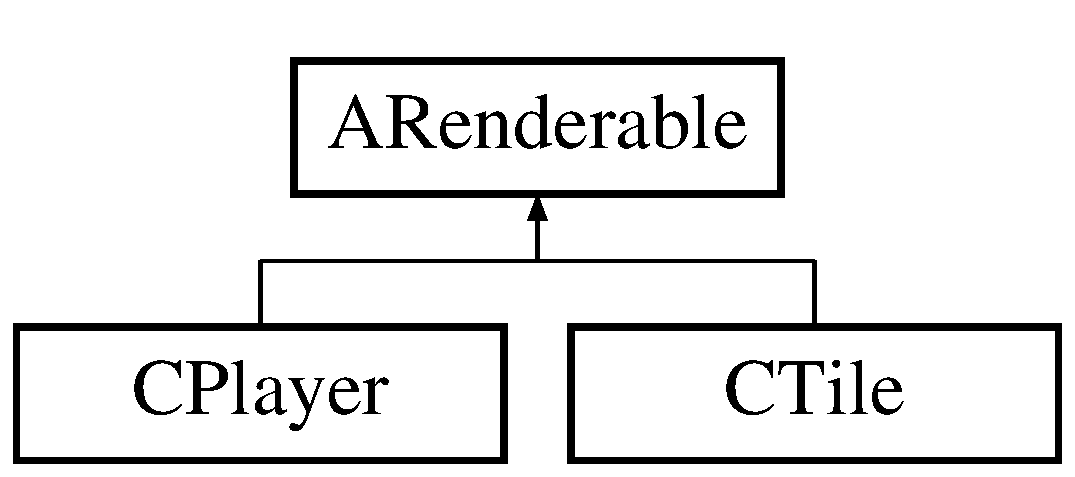
\includegraphics[height=2.000000cm]{classARenderable}
\end{center}
\end{figure}
\subsection*{Public Member Functions}
\begin{DoxyCompactItemize}
\item 
\hypertarget{classARenderable_a945fecfa1012fc94f186b8814f225ae8}{{\bfseries A\-Renderable} (\hyperlink{classCTexture}{C\-Texture} $\ast$p\-Texture, const sf\-::\-Vector2$<$ int $>$ \&curr\-Sub)}\label{classARenderable_a945fecfa1012fc94f186b8814f225ae8}

\item 
\hypertarget{classARenderable_a3d575592900ff1796452f35e7c618e6d}{\hyperlink{classARenderable_a3d575592900ff1796452f35e7c618e6d}{A\-Renderable} (\hyperlink{classCSprite}{C\-Sprite} $\ast$p\-Sprite)}\label{classARenderable_a3d575592900ff1796452f35e7c618e6d}

\begin{DoxyCompactList}\small\item\em if this constructor is used, note that this object then takes responsibility for the C\-Sprite$\ast$ \end{DoxyCompactList}\item 
\hypertarget{classARenderable_a4dc17477a94447c2ece7c418a47e3860}{\hyperlink{classCSprite}{C\-Sprite} $\ast$const {\bfseries get\-Sprite} ()}\label{classARenderable_a4dc17477a94447c2ece7c418a47e3860}

\item 
\hypertarget{classARenderable_a2cbb5617817d6697fd817f87bceebf77}{sf\-::\-Sprite $\ast$const \hyperlink{classARenderable_a2cbb5617817d6697fd817f87bceebf77}{get\-Sprite\-\_\-\-A\-P\-I} ()}\label{classARenderable_a2cbb5617817d6697fd817f87bceebf77}

\begin{DoxyCompactList}\small\item\em Returns the A\-P\-I version of this sprite. \end{DoxyCompactList}\item 
\hypertarget{classARenderable_a77d3d8b9f8d7f0e8b860abba2f6c53c9}{sf\-::\-Float\-Rect {\bfseries get\-Global\-Bounds} ()}\label{classARenderable_a77d3d8b9f8d7f0e8b860abba2f6c53c9}

\item 
\hypertarget{classARenderable_a1d0db7e6ba2e9bf6d8accb4164531b46}{void {\bfseries set\-Position} (float x, float y)}\label{classARenderable_a1d0db7e6ba2e9bf6d8accb4164531b46}

\end{DoxyCompactItemize}
\subsection*{Protected Attributes}
\begin{DoxyCompactItemize}
\item 
\hypertarget{classARenderable_a6030df923c81b400e94ff1f6a9df41f8}{\hyperlink{classCSprite}{C\-Sprite} $\ast$ {\bfseries m\-\_\-p\-Sprite}}\label{classARenderable_a6030df923c81b400e94ff1f6a9df41f8}

\end{DoxyCompactItemize}


\subsection{Detailed Description}


Definition at line 15 of file A\-Renderable.\-h.



The documentation for this class was generated from the following files\-:\begin{DoxyCompactItemize}
\item 
/home/z\-Zelman/\-Dropbox/\-Covert-\/\-Collisions Host dir/\-Covert-\/\-Collisions/src/\-Headers/A\-Renderable.\-h\item 
/home/z\-Zelman/\-Dropbox/\-Covert-\/\-Collisions Host dir/\-Covert-\/\-Collisions/src/\-Abstracts/A\-Renderable.\-cpp\end{DoxyCompactItemize}

\hypertarget{classAUpdate}{\section{A\-Update Class Reference}
\label{classAUpdate}\index{A\-Update@{A\-Update}}
}


Wrapper class to I\-Updatable which only adds 1 variable.  




{\ttfamily \#include $<$A\-Update.\-h$>$}



Inheritance diagram for A\-Update\-:
\nopagebreak
\begin{figure}[H]
\begin{center}
\leavevmode
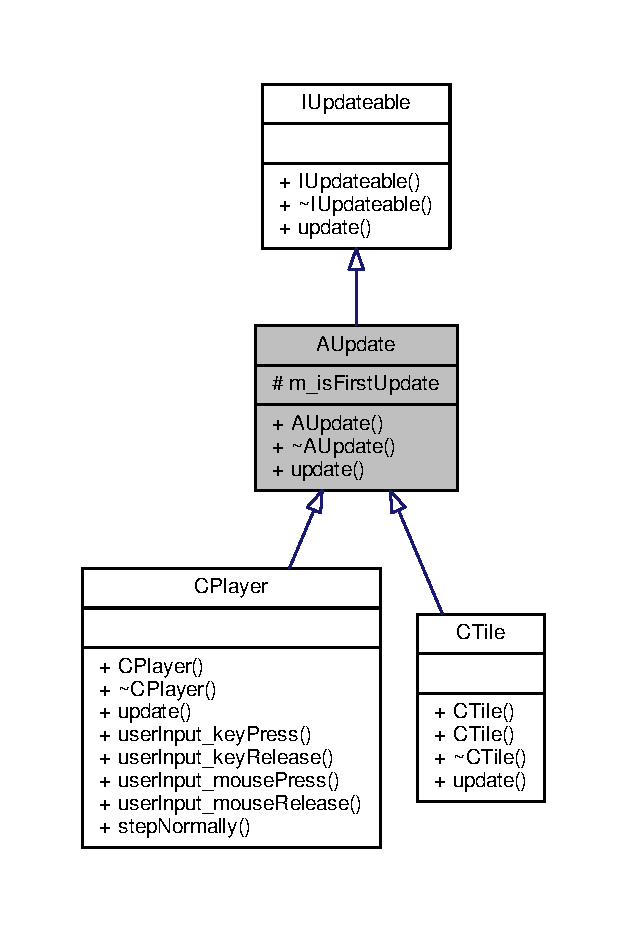
\includegraphics[width=301pt]{classAUpdate__inherit__graph}
\end{center}
\end{figure}


Collaboration diagram for A\-Update\-:
\nopagebreak
\begin{figure}[H]
\begin{center}
\leavevmode
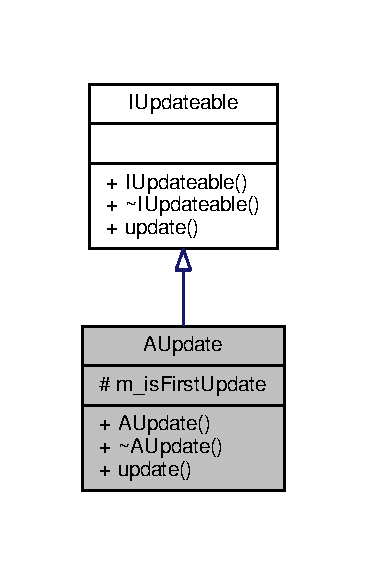
\includegraphics[width=176pt]{classAUpdate__coll__graph}
\end{center}
\end{figure}
\subsection*{Public Member Functions}
\begin{DoxyCompactItemize}
\item 
\hyperlink{classAUpdate_ac4d63cf5f9ca0bf2aeac2e61cdd8d981}{A\-Update} ()
\item 
virtual \hyperlink{classAUpdate_ab62e2d98b3711d172647442bb5889415}{$\sim$\-A\-Update} ()
\item 
virtual void \hyperlink{classAUpdate_a9f5be387e467fc5eea7fc45882abd949}{update} ()=0
\end{DoxyCompactItemize}
\subsection*{Protected Attributes}
\begin{DoxyCompactItemize}
\item 
bool \hyperlink{classAUpdate_adf0a017c2fd5abd12f64f7f0fd992e66}{m\-\_\-is\-First\-Update}
\begin{DoxyCompactList}\small\item\em Boolean to keep track of first-\/time update cycles. \end{DoxyCompactList}\end{DoxyCompactItemize}


\subsection{Detailed Description}
Wrapper class to I\-Updatable which only adds 1 variable. 

\begin{DoxySeeAlso}{See Also}
\hyperlink{classAUpdate_adf0a017c2fd5abd12f64f7f0fd992e66}{m\-\_\-is\-First\-Update} 
\end{DoxySeeAlso}


Definition at line 18 of file A\-Update.\-h.



\subsection{Constructor \& Destructor Documentation}
\hypertarget{classAUpdate_ac4d63cf5f9ca0bf2aeac2e61cdd8d981}{\index{A\-Update@{A\-Update}!A\-Update@{A\-Update}}
\index{A\-Update@{A\-Update}!AUpdate@{A\-Update}}
\subsubsection[{A\-Update}]{\setlength{\rightskip}{0pt plus 5cm}A\-Update\-::\-A\-Update (
\begin{DoxyParamCaption}
{}
\end{DoxyParamCaption}
)}}\label{classAUpdate_ac4d63cf5f9ca0bf2aeac2e61cdd8d981}


Definition at line 10 of file A\-Update.\-cpp.

\hypertarget{classAUpdate_ab62e2d98b3711d172647442bb5889415}{\index{A\-Update@{A\-Update}!$\sim$\-A\-Update@{$\sim$\-A\-Update}}
\index{$\sim$\-A\-Update@{$\sim$\-A\-Update}!AUpdate@{A\-Update}}
\subsubsection[{$\sim$\-A\-Update}]{\setlength{\rightskip}{0pt plus 5cm}A\-Update\-::$\sim$\-A\-Update (
\begin{DoxyParamCaption}
{}
\end{DoxyParamCaption}
)\hspace{0.3cm}{\ttfamily [virtual]}}}\label{classAUpdate_ab62e2d98b3711d172647442bb5889415}


Definition at line 16 of file A\-Update.\-cpp.



\subsection{Member Function Documentation}
\hypertarget{classAUpdate_a9f5be387e467fc5eea7fc45882abd949}{\index{A\-Update@{A\-Update}!update@{update}}
\index{update@{update}!AUpdate@{A\-Update}}
\subsubsection[{update}]{\setlength{\rightskip}{0pt plus 5cm}virtual void A\-Update\-::update (
\begin{DoxyParamCaption}
{}
\end{DoxyParamCaption}
)\hspace{0.3cm}{\ttfamily [pure virtual]}}}\label{classAUpdate_a9f5be387e467fc5eea7fc45882abd949}


Implements \hyperlink{classIUpdateable_a46d178a1ecdab33bcaad25d9b38582a5}{I\-Updateable}.



Implemented in \hyperlink{classCTile_a818a17e48a7219eedac950b82c641ee0}{C\-Tile}, and \hyperlink{classCPlayer_aa77025c046956b109a76d53c12a80fa5}{C\-Player}.



\subsection{Member Data Documentation}
\hypertarget{classAUpdate_adf0a017c2fd5abd12f64f7f0fd992e66}{\index{A\-Update@{A\-Update}!m\-\_\-is\-First\-Update@{m\-\_\-is\-First\-Update}}
\index{m\-\_\-is\-First\-Update@{m\-\_\-is\-First\-Update}!AUpdate@{A\-Update}}
\subsubsection[{m\-\_\-is\-First\-Update}]{\setlength{\rightskip}{0pt plus 5cm}bool A\-Update\-::m\-\_\-is\-First\-Update\hspace{0.3cm}{\ttfamily [protected]}}}\label{classAUpdate_adf0a017c2fd5abd12f64f7f0fd992e66}


Boolean to keep track of first-\/time update cycles. 

This is intended to prevent time-\/sensitive things from freaking out from the objects init time to the first update 

Definition at line 34 of file A\-Update.\-h.



The documentation for this class was generated from the following files\-:\begin{DoxyCompactItemize}
\item 
/home/z\-Zelman/\-Dropbox/\-Covert-\/\-Collisions Host dir/\-Covert-\/\-Collisions/src/\-Headers/\hyperlink{AUpdate_8h}{A\-Update.\-h}\item 
/home/z\-Zelman/\-Dropbox/\-Covert-\/\-Collisions Host dir/\-Covert-\/\-Collisions/src/\-Abstracts/\hyperlink{AUpdate_8cpp}{A\-Update.\-cpp}\end{DoxyCompactItemize}

\hypertarget{classAUserInput}{\section{A\-User\-Input Class Reference}
\label{classAUserInput}\index{A\-User\-Input@{A\-User\-Input}}
}


Abstract class which decomposes the different types of user input.  




{\ttfamily \#include $<$A\-User\-Input.\-h$>$}



Inheritance diagram for A\-User\-Input\-:\nopagebreak
\begin{figure}[H]
\begin{center}
\leavevmode
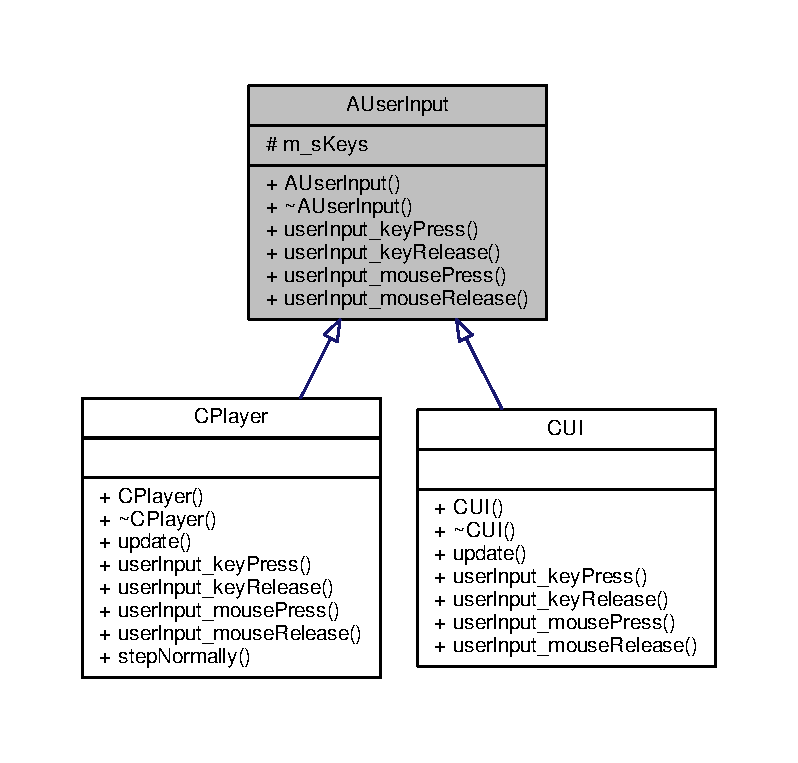
\includegraphics[width=350pt]{classAUserInput__inherit__graph}
\end{center}
\end{figure}


Collaboration diagram for A\-User\-Input\-:\nopagebreak
\begin{figure}[H]
\begin{center}
\leavevmode
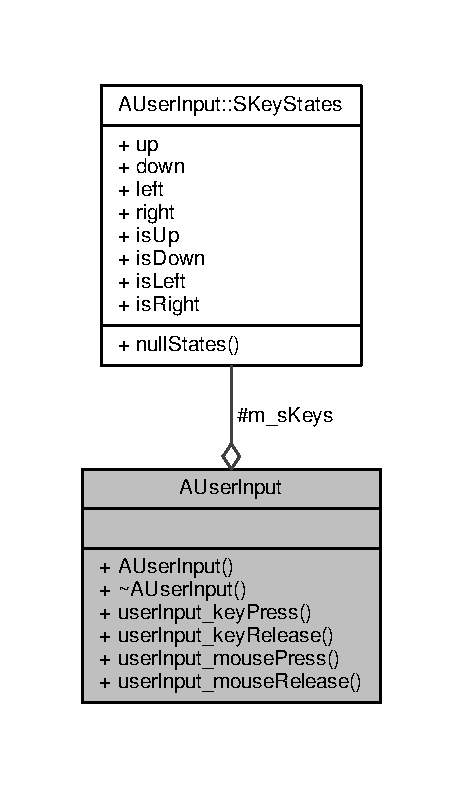
\includegraphics[width=222pt]{classAUserInput__coll__graph}
\end{center}
\end{figure}
\subsection*{Classes}
\begin{DoxyCompactItemize}
\item 
struct \hyperlink{structAUserInput_1_1SKeyStates}{S\-Key\-States}
\begin{DoxyCompactList}\small\item\em Representation of acceptable key presses, and states of those keys. \end{DoxyCompactList}\end{DoxyCompactItemize}
\subsection*{Public Member Functions}
\begin{DoxyCompactItemize}
\item 
\hyperlink{classAUserInput_a83cdb578d5ff8c37f1fb219234d7319b}{A\-User\-Input} ()
\item 
virtual \hyperlink{classAUserInput_a8e45374f4f78942389badab10fa1ef04}{$\sim$\-A\-User\-Input} ()
\item 
virtual bool \hyperlink{classAUserInput_a110239bcc0461666583d1dc940cb5d13}{user\-Input\-\_\-key\-Press} (sf\-::\-Event $\ast$p\-Event)=0
\item 
virtual bool \hyperlink{classAUserInput_afe8ae22fff673d788e366b9b29ffa67d}{user\-Input\-\_\-key\-Release} (sf\-::\-Event $\ast$p\-Event)=0
\item 
virtual bool \hyperlink{classAUserInput_a567e0d0610bd2ef2e23fed64b3e56d2b}{user\-Input\-\_\-mouse\-Press} (sf\-::\-Event $\ast$p\-Event)=0
\item 
virtual bool \hyperlink{classAUserInput_a570f71dde4825c3e9bdcf6b58857f514}{user\-Input\-\_\-mouse\-Release} (sf\-::\-Event $\ast$p\-Event)=0
\end{DoxyCompactItemize}
\subsection*{Protected Attributes}
\begin{DoxyCompactItemize}
\item 
struct \hyperlink{structAUserInput_1_1SKeyStates}{A\-User\-Input\-::\-S\-Key\-States} \hyperlink{classAUserInput_a55b881326b920413bbcdf6e02c4fb021}{m\-\_\-s\-Keys}
\end{DoxyCompactItemize}


\subsection{Detailed Description}
Abstract class which decomposes the different types of user input. 

Definition at line 16 of file A\-User\-Input.\-h.



\subsection{Constructor \& Destructor Documentation}
\hypertarget{classAUserInput_a83cdb578d5ff8c37f1fb219234d7319b}{\index{A\-User\-Input@{A\-User\-Input}!A\-User\-Input@{A\-User\-Input}}
\index{A\-User\-Input@{A\-User\-Input}!AUserInput@{A\-User\-Input}}
\subsubsection[{A\-User\-Input}]{\setlength{\rightskip}{0pt plus 5cm}A\-User\-Input\-::\-A\-User\-Input (
\begin{DoxyParamCaption}
{}
\end{DoxyParamCaption}
)}}\label{classAUserInput_a83cdb578d5ff8c37f1fb219234d7319b}


Definition at line 10 of file A\-User\-Input.\-cpp.

\hypertarget{classAUserInput_a8e45374f4f78942389badab10fa1ef04}{\index{A\-User\-Input@{A\-User\-Input}!$\sim$\-A\-User\-Input@{$\sim$\-A\-User\-Input}}
\index{$\sim$\-A\-User\-Input@{$\sim$\-A\-User\-Input}!AUserInput@{A\-User\-Input}}
\subsubsection[{$\sim$\-A\-User\-Input}]{\setlength{\rightskip}{0pt plus 5cm}A\-User\-Input\-::$\sim$\-A\-User\-Input (
\begin{DoxyParamCaption}
{}
\end{DoxyParamCaption}
)\hspace{0.3cm}{\ttfamily [virtual]}}}\label{classAUserInput_a8e45374f4f78942389badab10fa1ef04}


Definition at line 16 of file A\-User\-Input.\-cpp.



\subsection{Member Function Documentation}
\hypertarget{classAUserInput_a110239bcc0461666583d1dc940cb5d13}{\index{A\-User\-Input@{A\-User\-Input}!user\-Input\-\_\-key\-Press@{user\-Input\-\_\-key\-Press}}
\index{user\-Input\-\_\-key\-Press@{user\-Input\-\_\-key\-Press}!AUserInput@{A\-User\-Input}}
\subsubsection[{user\-Input\-\_\-key\-Press}]{\setlength{\rightskip}{0pt plus 5cm}virtual bool A\-User\-Input\-::user\-Input\-\_\-key\-Press (
\begin{DoxyParamCaption}
\item[{sf\-::\-Event $\ast$}]{p\-Event}
\end{DoxyParamCaption}
)\hspace{0.3cm}{\ttfamily [pure virtual]}}}\label{classAUserInput_a110239bcc0461666583d1dc940cb5d13}


Implemented in \hyperlink{classCPlayer_ab91fc8d3c4e992dd20270d5743d75f06}{C\-Player}, and \hyperlink{classCUI_addb1531f20541cb7c7f8688f1cd843e9}{C\-U\-I}.

\hypertarget{classAUserInput_afe8ae22fff673d788e366b9b29ffa67d}{\index{A\-User\-Input@{A\-User\-Input}!user\-Input\-\_\-key\-Release@{user\-Input\-\_\-key\-Release}}
\index{user\-Input\-\_\-key\-Release@{user\-Input\-\_\-key\-Release}!AUserInput@{A\-User\-Input}}
\subsubsection[{user\-Input\-\_\-key\-Release}]{\setlength{\rightskip}{0pt plus 5cm}virtual bool A\-User\-Input\-::user\-Input\-\_\-key\-Release (
\begin{DoxyParamCaption}
\item[{sf\-::\-Event $\ast$}]{p\-Event}
\end{DoxyParamCaption}
)\hspace{0.3cm}{\ttfamily [pure virtual]}}}\label{classAUserInput_afe8ae22fff673d788e366b9b29ffa67d}


Implemented in \hyperlink{classCPlayer_a8ef81a467d70f1e4529f3c905820311b}{C\-Player}, and \hyperlink{classCUI_a0495bb6ad5fba9ef0552a487151f7896}{C\-U\-I}.

\hypertarget{classAUserInput_a567e0d0610bd2ef2e23fed64b3e56d2b}{\index{A\-User\-Input@{A\-User\-Input}!user\-Input\-\_\-mouse\-Press@{user\-Input\-\_\-mouse\-Press}}
\index{user\-Input\-\_\-mouse\-Press@{user\-Input\-\_\-mouse\-Press}!AUserInput@{A\-User\-Input}}
\subsubsection[{user\-Input\-\_\-mouse\-Press}]{\setlength{\rightskip}{0pt plus 5cm}virtual bool A\-User\-Input\-::user\-Input\-\_\-mouse\-Press (
\begin{DoxyParamCaption}
\item[{sf\-::\-Event $\ast$}]{p\-Event}
\end{DoxyParamCaption}
)\hspace{0.3cm}{\ttfamily [pure virtual]}}}\label{classAUserInput_a567e0d0610bd2ef2e23fed64b3e56d2b}


Implemented in \hyperlink{classCPlayer_ab73ca18309b25410b1fdb54a9ee60e67}{C\-Player}, and \hyperlink{classCUI_a6edfa48bb429f6e1468f5c3568cf83c5}{C\-U\-I}.

\hypertarget{classAUserInput_a570f71dde4825c3e9bdcf6b58857f514}{\index{A\-User\-Input@{A\-User\-Input}!user\-Input\-\_\-mouse\-Release@{user\-Input\-\_\-mouse\-Release}}
\index{user\-Input\-\_\-mouse\-Release@{user\-Input\-\_\-mouse\-Release}!AUserInput@{A\-User\-Input}}
\subsubsection[{user\-Input\-\_\-mouse\-Release}]{\setlength{\rightskip}{0pt plus 5cm}virtual bool A\-User\-Input\-::user\-Input\-\_\-mouse\-Release (
\begin{DoxyParamCaption}
\item[{sf\-::\-Event $\ast$}]{p\-Event}
\end{DoxyParamCaption}
)\hspace{0.3cm}{\ttfamily [pure virtual]}}}\label{classAUserInput_a570f71dde4825c3e9bdcf6b58857f514}


Implemented in \hyperlink{classCPlayer_a915cf5ad902cddb376eb4c37d362e3b1}{C\-Player}, and \hyperlink{classCUI_a64e3c8ad256e2d814e7112d201cb78ae}{C\-U\-I}.



\subsection{Member Data Documentation}
\hypertarget{classAUserInput_a55b881326b920413bbcdf6e02c4fb021}{\index{A\-User\-Input@{A\-User\-Input}!m\-\_\-s\-Keys@{m\-\_\-s\-Keys}}
\index{m\-\_\-s\-Keys@{m\-\_\-s\-Keys}!AUserInput@{A\-User\-Input}}
\subsubsection[{m\-\_\-s\-Keys}]{\setlength{\rightskip}{0pt plus 5cm}struct {\bf A\-User\-Input\-::\-S\-Key\-States}  A\-User\-Input\-::m\-\_\-s\-Keys\hspace{0.3cm}{\ttfamily [protected]}}}\label{classAUserInput_a55b881326b920413bbcdf6e02c4fb021}


The documentation for this class was generated from the following files\-:\begin{DoxyCompactItemize}
\item 
/home/z\-Zelman/\-Dropbox/\-Covert-\/\-Collisions Host dir/\-Covert-\/\-Collisions/src/\-Headers/\hyperlink{AUserInput_8h}{A\-User\-Input.\-h}\item 
/home/z\-Zelman/\-Dropbox/\-Covert-\/\-Collisions Host dir/\-Covert-\/\-Collisions/src/\-Abstracts/\hyperlink{AUserInput_8cpp}{A\-User\-Input.\-cpp}\end{DoxyCompactItemize}

\hypertarget{classCGame}{\section{C\-Game Class Reference}
\label{classCGame}\index{C\-Game@{C\-Game}}
}
\subsection*{Public Member Functions}
\begin{DoxyCompactItemize}
\item 
\hypertarget{classCGame_a9ed0bb7ef800bc7e568cf8858c3b96ec}{sf\-::\-Render\-Window $\ast$ {\bfseries get\-Game\-Window} ()}\label{classCGame_a9ed0bb7ef800bc7e568cf8858c3b96ec}

\item 
\hypertarget{classCGame_ae45938d7b77b13d2e80e4f9b3a17a44a}{bool {\bfseries get\-Is\-Running} ()}\label{classCGame_ae45938d7b77b13d2e80e4f9b3a17a44a}

\item 
\hypertarget{classCGame_a9b2f241693b1f024c957f92069fe6ed7}{bool {\bfseries get\-Is\-Paused} ()}\label{classCGame_a9b2f241693b1f024c957f92069fe6ed7}

\item 
\hypertarget{classCGame_aa94f04e2c012603f10430a4d4db3ce27}{void {\bfseries start\-Game} ()}\label{classCGame_aa94f04e2c012603f10430a4d4db3ce27}

\item 
\hypertarget{classCGame_acbad86ee58748e2db0da540f4aa0640e}{void {\bfseries stop\-Game} ()}\label{classCGame_acbad86ee58748e2db0da540f4aa0640e}

\end{DoxyCompactItemize}


\subsection{Detailed Description}


Definition at line 22 of file C\-Game.\-h.



The documentation for this class was generated from the following files\-:\begin{DoxyCompactItemize}
\item 
/home/z\-Zelman/\-Dropbox/\-Covert-\/\-Collisions Host dir/\-Covert-\/\-Collisions/src/C\-Game.\-h\item 
/home/z\-Zelman/\-Dropbox/\-Covert-\/\-Collisions Host dir/\-Covert-\/\-Collisions/src/C\-Game.\-cpp\end{DoxyCompactItemize}

\hypertarget{classCPhysicsEngine}{\section{C\-Physics\-Engine Class Reference}
\label{classCPhysicsEngine}\index{C\-Physics\-Engine@{C\-Physics\-Engine}}
}


Module of the game engine that is responsible for\-: resolving collisions and updating physics data within objects.  




{\ttfamily \#include $<$C\-Physics\-Engine.\-h$>$}



Inheritance diagram for C\-Physics\-Engine\-:
\nopagebreak
\begin{figure}[H]
\begin{center}
\leavevmode
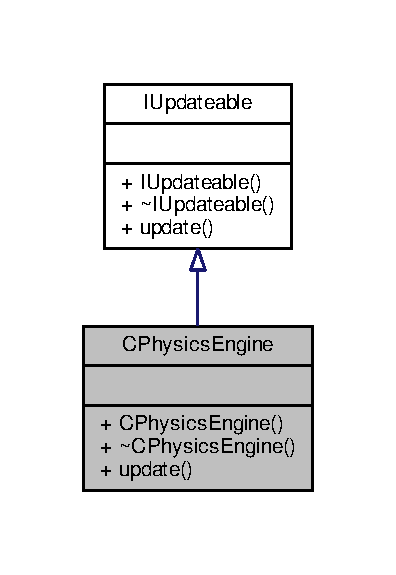
\includegraphics[width=190pt]{classCPhysicsEngine__inherit__graph}
\end{center}
\end{figure}


Collaboration diagram for C\-Physics\-Engine\-:
\nopagebreak
\begin{figure}[H]
\begin{center}
\leavevmode
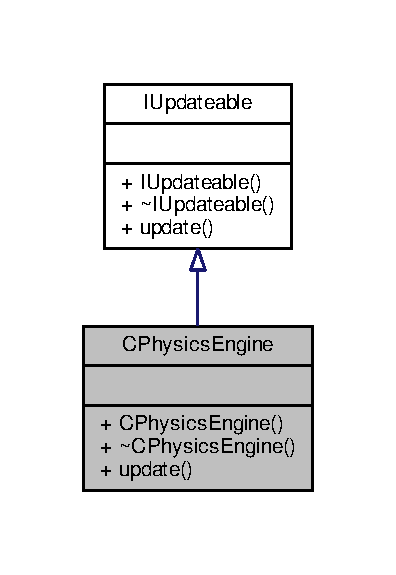
\includegraphics[width=190pt]{classCPhysicsEngine__coll__graph}
\end{center}
\end{figure}
\subsection*{Public Member Functions}
\begin{DoxyCompactItemize}
\item 
\hyperlink{classCPhysicsEngine_ab7a2fa6ebd7e1ad0da2ab36d92ae8608}{C\-Physics\-Engine} (\hyperlink{classCPlayer}{C\-Player} $\ast$p\-Player, \hyperlink{classCTile__Container}{C\-Tile\-\_\-\-Container} $\ast$p\-Tile\-\_\-\-Container)
\item 
\hyperlink{classCPhysicsEngine_a2e432f93b60e9e38a8882223ea3ee71b}{$\sim$\-C\-Physics\-Engine} ()
\item 
void \hyperlink{classCPhysicsEngine_abc493897bbdb15e6787a25478730f1f5}{update} ()
\begin{DoxyCompactList}\small\item\em Only updates the velocities within the objects, and calls \char`\"{}step\-Normally()\char`\"{} if it can step normally within the next update. \end{DoxyCompactList}\end{DoxyCompactItemize}


\subsection{Detailed Description}
Module of the game engine that is responsible for\-: resolving collisions and updating physics data within objects. 

Definition at line 21 of file C\-Physics\-Engine.\-h.



\subsection{Constructor \& Destructor Documentation}
\hypertarget{classCPhysicsEngine_ab7a2fa6ebd7e1ad0da2ab36d92ae8608}{\index{C\-Physics\-Engine@{C\-Physics\-Engine}!C\-Physics\-Engine@{C\-Physics\-Engine}}
\index{C\-Physics\-Engine@{C\-Physics\-Engine}!CPhysicsEngine@{C\-Physics\-Engine}}
\subsubsection[{C\-Physics\-Engine}]{\setlength{\rightskip}{0pt plus 5cm}C\-Physics\-Engine\-::\-C\-Physics\-Engine (
\begin{DoxyParamCaption}
\item[{{\bf C\-Player} $\ast$}]{p\-Player, }
\item[{{\bf C\-Tile\-\_\-\-Container} $\ast$}]{p\-Tile\-\_\-\-Container}
\end{DoxyParamCaption}
)}}\label{classCPhysicsEngine_ab7a2fa6ebd7e1ad0da2ab36d92ae8608}


Definition at line 11 of file C\-Physics\-Engine.\-cpp.

\hypertarget{classCPhysicsEngine_a2e432f93b60e9e38a8882223ea3ee71b}{\index{C\-Physics\-Engine@{C\-Physics\-Engine}!$\sim$\-C\-Physics\-Engine@{$\sim$\-C\-Physics\-Engine}}
\index{$\sim$\-C\-Physics\-Engine@{$\sim$\-C\-Physics\-Engine}!CPhysicsEngine@{C\-Physics\-Engine}}
\subsubsection[{$\sim$\-C\-Physics\-Engine}]{\setlength{\rightskip}{0pt plus 5cm}C\-Physics\-Engine\-::$\sim$\-C\-Physics\-Engine (
\begin{DoxyParamCaption}
{}
\end{DoxyParamCaption}
)}}\label{classCPhysicsEngine_a2e432f93b60e9e38a8882223ea3ee71b}


Definition at line 21 of file C\-Physics\-Engine.\-cpp.



\subsection{Member Function Documentation}
\hypertarget{classCPhysicsEngine_abc493897bbdb15e6787a25478730f1f5}{\index{C\-Physics\-Engine@{C\-Physics\-Engine}!update@{update}}
\index{update@{update}!CPhysicsEngine@{C\-Physics\-Engine}}
\subsubsection[{update}]{\setlength{\rightskip}{0pt plus 5cm}void C\-Physics\-Engine\-::update (
\begin{DoxyParamCaption}
{}
\end{DoxyParamCaption}
)\hspace{0.3cm}{\ttfamily [virtual]}}}\label{classCPhysicsEngine_abc493897bbdb15e6787a25478730f1f5}


Only updates the velocities within the objects, and calls \char`\"{}step\-Normally()\char`\"{} if it can step normally within the next update. 

Does not call the object's \char`\"{}update()\char`\"{} function!! 

Implements \hyperlink{classIUpdateable_a46d178a1ecdab33bcaad25d9b38582a5}{I\-Updateable}.



Definition at line 26 of file C\-Physics\-Engine.\-cpp.



The documentation for this class was generated from the following files\-:\begin{DoxyCompactItemize}
\item 
/home/z\-Zelman/\-Dropbox/\-Covert-\/\-Collisions Host dir/\-Covert-\/\-Collisions/src/\-Headers/\hyperlink{CPhysicsEngine_8h}{C\-Physics\-Engine.\-h}\item 
/home/z\-Zelman/\-Dropbox/\-Covert-\/\-Collisions Host dir/\-Covert-\/\-Collisions/src/\-Physics/\hyperlink{CPhysicsEngine_8cpp}{C\-Physics\-Engine.\-cpp}\end{DoxyCompactItemize}

\hypertarget{classCPlayer}{\section{C\-Player Class Reference}
\label{classCPlayer}\index{C\-Player@{C\-Player}}
}


Base class of each individual player.  




{\ttfamily \#include $<$C\-Player.\-h$>$}



Inheritance diagram for C\-Player\-:
\nopagebreak
\begin{figure}[H]
\begin{center}
\leavevmode
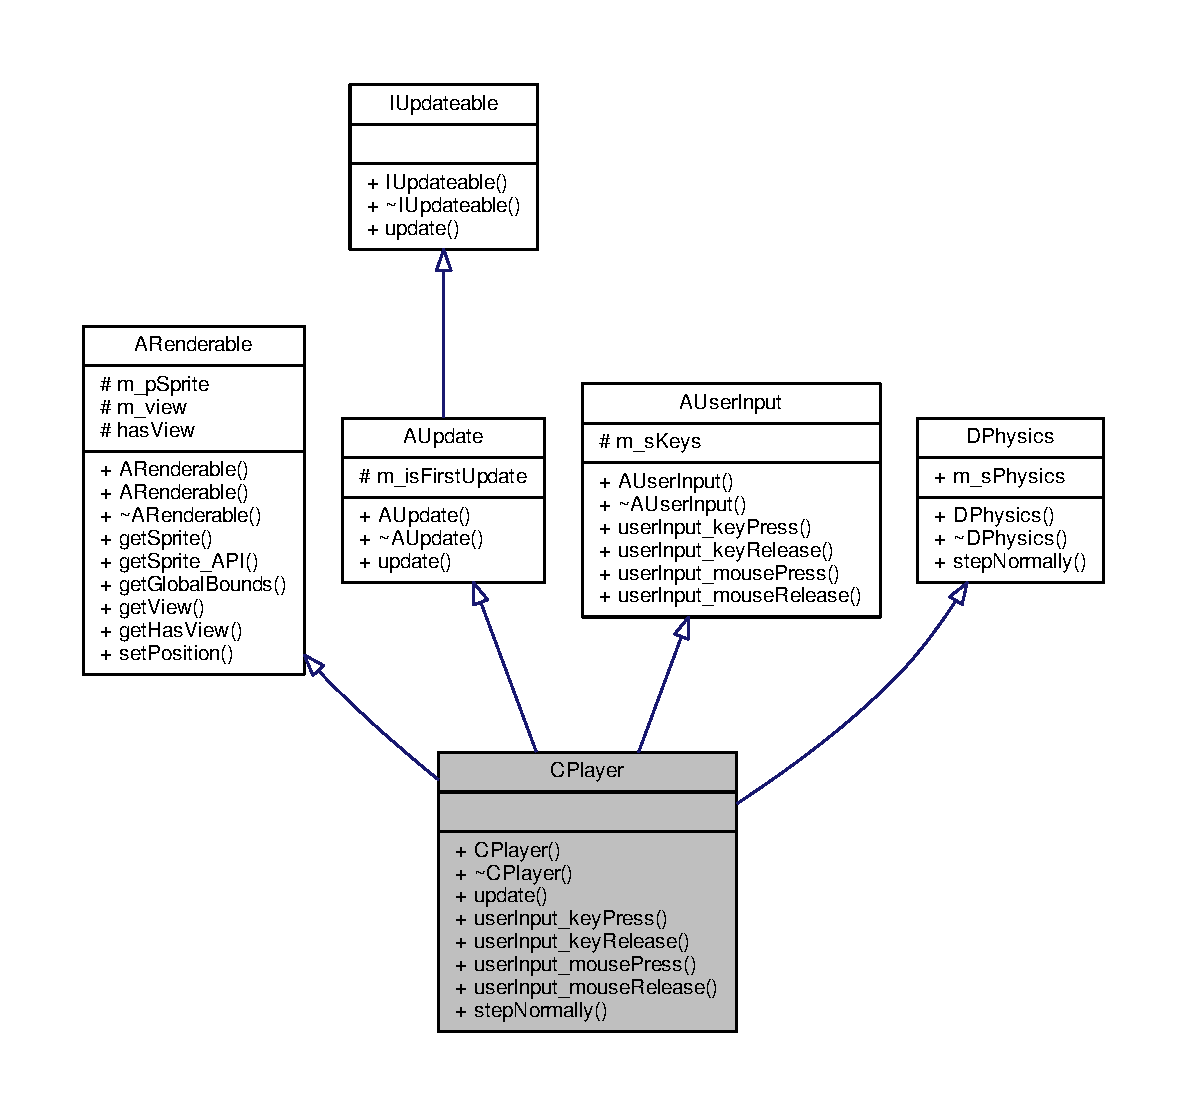
\includegraphics[width=350pt]{classCPlayer__inherit__graph}
\end{center}
\end{figure}


Collaboration diagram for C\-Player\-:
\nopagebreak
\begin{figure}[H]
\begin{center}
\leavevmode
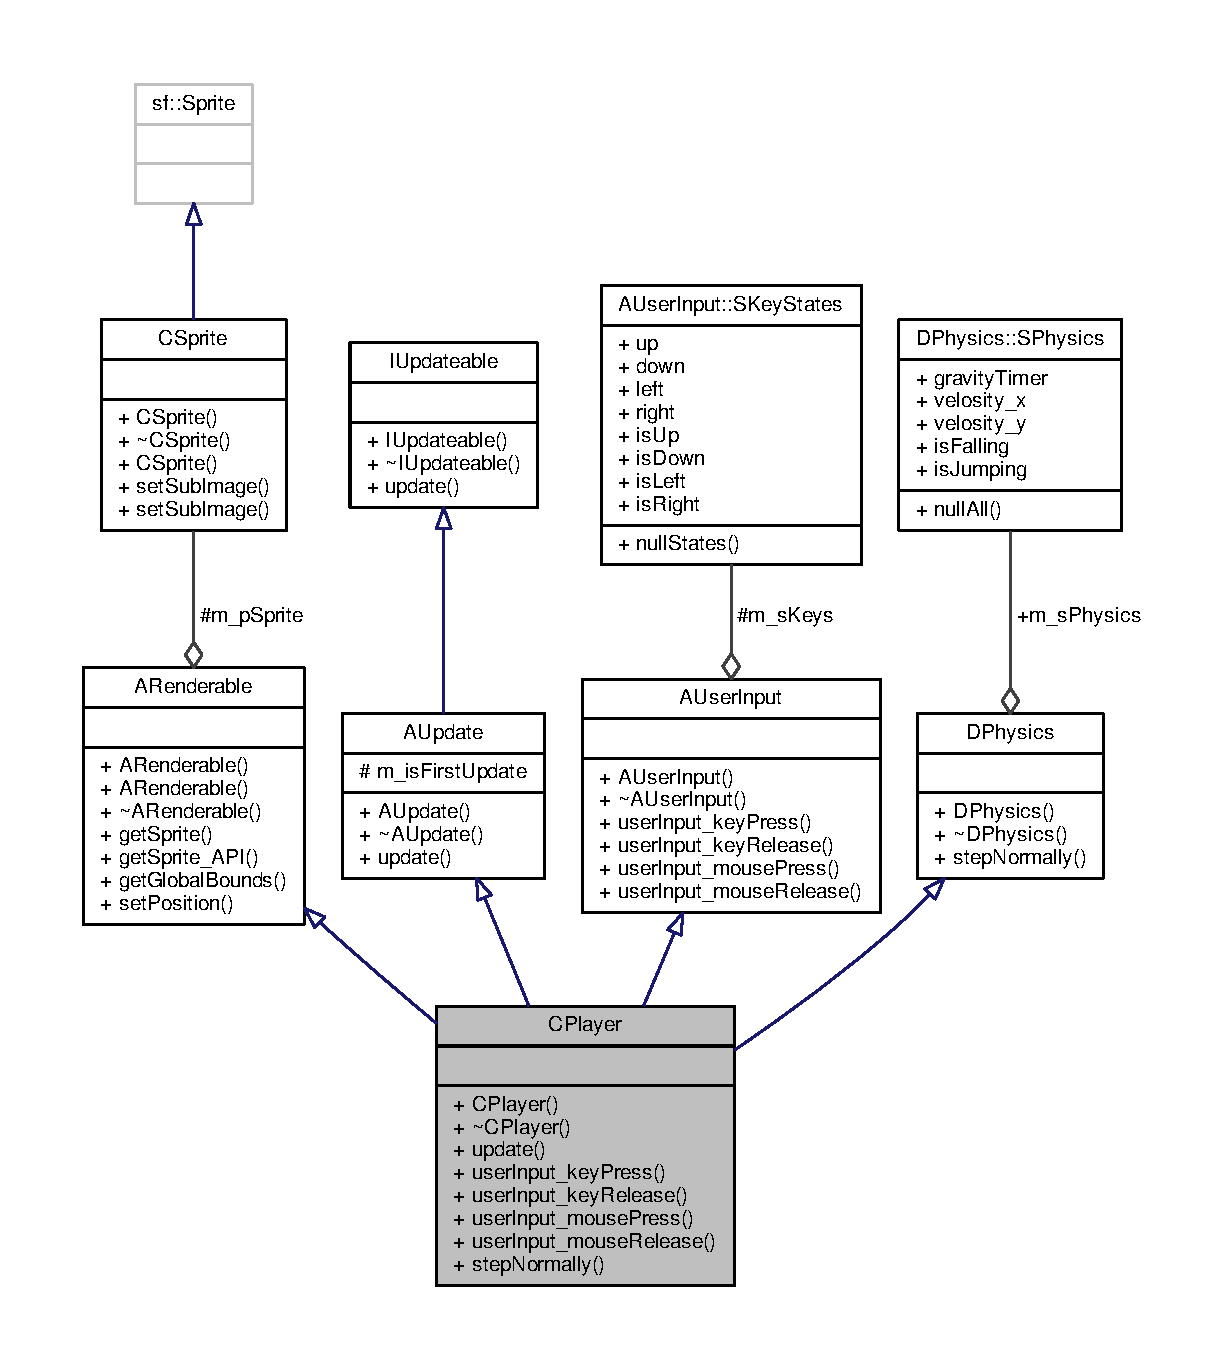
\includegraphics[width=350pt]{classCPlayer__coll__graph}
\end{center}
\end{figure}
\subsection*{Public Member Functions}
\begin{DoxyCompactItemize}
\item 
\hyperlink{classCPlayer_a983c63a3e18585a94f66f0bd23c57cd3}{C\-Player} (\hyperlink{classCTexture}{C\-Texture} $\ast$p\-Texture, const sf\-::\-Vector2$<$ int $>$ \&curr\-Sub)
\item 
\hyperlink{classCPlayer_ad02df04887bccfe3b82298895da24af6}{$\sim$\-C\-Player} ()
\item 
void \hyperlink{classCPlayer_aa77025c046956b109a76d53c12a80fa5}{update} ()
\begin{DoxyCompactList}\small\item\em Function to update object state each update cycle. \end{DoxyCompactList}\item 
bool \hyperlink{classCPlayer_ab91fc8d3c4e992dd20270d5743d75f06}{user\-Input\-\_\-key\-Press} (sf\-::\-Event $\ast$p\-Event)
\item 
bool \hyperlink{classCPlayer_a8ef81a467d70f1e4529f3c905820311b}{user\-Input\-\_\-key\-Release} (sf\-::\-Event $\ast$p\-Event)
\item 
bool \hyperlink{classCPlayer_ab73ca18309b25410b1fdb54a9ee60e67}{user\-Input\-\_\-mouse\-Press} (sf\-::\-Event $\ast$p\-Event)
\item 
bool \hyperlink{classCPlayer_a915cf5ad902cddb376eb4c37d362e3b1}{user\-Input\-\_\-mouse\-Release} (sf\-::\-Event $\ast$p\-Event)
\item 
void \hyperlink{classCPlayer_aedadef185076d940923e9402a15cdf90}{step\-Normally} ()
\begin{DoxyCompactList}\small\item\em A normal step in 1 update call. \end{DoxyCompactList}\end{DoxyCompactItemize}
\subsection*{Additional Inherited Members}


\subsection{Detailed Description}
Base class of each individual player. 

The player is the thing that the human person controls in the game world 

Definition at line 23 of file C\-Player.\-h.



\subsection{Constructor \& Destructor Documentation}
\hypertarget{classCPlayer_a983c63a3e18585a94f66f0bd23c57cd3}{\index{C\-Player@{C\-Player}!C\-Player@{C\-Player}}
\index{C\-Player@{C\-Player}!CPlayer@{C\-Player}}
\subsubsection[{C\-Player}]{\setlength{\rightskip}{0pt plus 5cm}C\-Player\-::\-C\-Player (
\begin{DoxyParamCaption}
\item[{{\bf C\-Texture} $\ast$}]{p\-Texture, }
\item[{const sf\-::\-Vector2$<$ int $>$ \&}]{curr\-Sub}
\end{DoxyParamCaption}
)}}\label{classCPlayer_a983c63a3e18585a94f66f0bd23c57cd3}


Definition at line 11 of file C\-Player.\-cpp.

\hypertarget{classCPlayer_ad02df04887bccfe3b82298895da24af6}{\index{C\-Player@{C\-Player}!$\sim$\-C\-Player@{$\sim$\-C\-Player}}
\index{$\sim$\-C\-Player@{$\sim$\-C\-Player}!CPlayer@{C\-Player}}
\subsubsection[{$\sim$\-C\-Player}]{\setlength{\rightskip}{0pt plus 5cm}C\-Player\-::$\sim$\-C\-Player (
\begin{DoxyParamCaption}
{}
\end{DoxyParamCaption}
)}}\label{classCPlayer_ad02df04887bccfe3b82298895da24af6}


Definition at line 25 of file C\-Player.\-cpp.



\subsection{Member Function Documentation}
\hypertarget{classCPlayer_aedadef185076d940923e9402a15cdf90}{\index{C\-Player@{C\-Player}!step\-Normally@{step\-Normally}}
\index{step\-Normally@{step\-Normally}!CPlayer@{C\-Player}}
\subsubsection[{step\-Normally}]{\setlength{\rightskip}{0pt plus 5cm}void C\-Player\-::step\-Normally (
\begin{DoxyParamCaption}
{}
\end{DoxyParamCaption}
)\hspace{0.3cm}{\ttfamily [virtual]}}}\label{classCPlayer_aedadef185076d940923e9402a15cdf90}


A normal step in 1 update call. 

When this method is called, it is assumed that there will N\-O\-T be a collision during 1 step. 

Implements \hyperlink{classDPhysics_a414316ffcec06dbf01ced086bbb92b55}{D\-Physics}.



Definition at line 136 of file C\-Player.\-cpp.

\hypertarget{classCPlayer_aa77025c046956b109a76d53c12a80fa5}{\index{C\-Player@{C\-Player}!update@{update}}
\index{update@{update}!CPlayer@{C\-Player}}
\subsubsection[{update}]{\setlength{\rightskip}{0pt plus 5cm}void C\-Player\-::update (
\begin{DoxyParamCaption}
{}
\end{DoxyParamCaption}
)\hspace{0.3cm}{\ttfamily [virtual]}}}\label{classCPlayer_aa77025c046956b109a76d53c12a80fa5}


Function to update object state each update cycle. 



Implements \hyperlink{classAUpdate_a9f5be387e467fc5eea7fc45882abd949}{A\-Update}.



Definition at line 148 of file C\-Player.\-cpp.

\hypertarget{classCPlayer_ab91fc8d3c4e992dd20270d5743d75f06}{\index{C\-Player@{C\-Player}!user\-Input\-\_\-key\-Press@{user\-Input\-\_\-key\-Press}}
\index{user\-Input\-\_\-key\-Press@{user\-Input\-\_\-key\-Press}!CPlayer@{C\-Player}}
\subsubsection[{user\-Input\-\_\-key\-Press}]{\setlength{\rightskip}{0pt plus 5cm}bool C\-Player\-::user\-Input\-\_\-key\-Press (
\begin{DoxyParamCaption}
\item[{sf\-::\-Event $\ast$}]{p\-Event}
\end{DoxyParamCaption}
)\hspace{0.3cm}{\ttfamily [virtual]}}}\label{classCPlayer_ab91fc8d3c4e992dd20270d5743d75f06}


Implements \hyperlink{classAUserInput_a110239bcc0461666583d1dc940cb5d13}{A\-User\-Input}.



Definition at line 41 of file C\-Player.\-cpp.

\hypertarget{classCPlayer_a8ef81a467d70f1e4529f3c905820311b}{\index{C\-Player@{C\-Player}!user\-Input\-\_\-key\-Release@{user\-Input\-\_\-key\-Release}}
\index{user\-Input\-\_\-key\-Release@{user\-Input\-\_\-key\-Release}!CPlayer@{C\-Player}}
\subsubsection[{user\-Input\-\_\-key\-Release}]{\setlength{\rightskip}{0pt plus 5cm}bool C\-Player\-::user\-Input\-\_\-key\-Release (
\begin{DoxyParamCaption}
\item[{sf\-::\-Event $\ast$}]{p\-Event}
\end{DoxyParamCaption}
)\hspace{0.3cm}{\ttfamily [virtual]}}}\label{classCPlayer_a8ef81a467d70f1e4529f3c905820311b}


Implements \hyperlink{classAUserInput_afe8ae22fff673d788e366b9b29ffa67d}{A\-User\-Input}.



Definition at line 83 of file C\-Player.\-cpp.

\hypertarget{classCPlayer_ab73ca18309b25410b1fdb54a9ee60e67}{\index{C\-Player@{C\-Player}!user\-Input\-\_\-mouse\-Press@{user\-Input\-\_\-mouse\-Press}}
\index{user\-Input\-\_\-mouse\-Press@{user\-Input\-\_\-mouse\-Press}!CPlayer@{C\-Player}}
\subsubsection[{user\-Input\-\_\-mouse\-Press}]{\setlength{\rightskip}{0pt plus 5cm}bool C\-Player\-::user\-Input\-\_\-mouse\-Press (
\begin{DoxyParamCaption}
\item[{sf\-::\-Event $\ast$}]{p\-Event}
\end{DoxyParamCaption}
)\hspace{0.3cm}{\ttfamily [virtual]}}}\label{classCPlayer_ab73ca18309b25410b1fdb54a9ee60e67}


Implements \hyperlink{classAUserInput_a567e0d0610bd2ef2e23fed64b3e56d2b}{A\-User\-Input}.



Definition at line 124 of file C\-Player.\-cpp.

\hypertarget{classCPlayer_a915cf5ad902cddb376eb4c37d362e3b1}{\index{C\-Player@{C\-Player}!user\-Input\-\_\-mouse\-Release@{user\-Input\-\_\-mouse\-Release}}
\index{user\-Input\-\_\-mouse\-Release@{user\-Input\-\_\-mouse\-Release}!CPlayer@{C\-Player}}
\subsubsection[{user\-Input\-\_\-mouse\-Release}]{\setlength{\rightskip}{0pt plus 5cm}bool C\-Player\-::user\-Input\-\_\-mouse\-Release (
\begin{DoxyParamCaption}
\item[{sf\-::\-Event $\ast$}]{p\-Event}
\end{DoxyParamCaption}
)\hspace{0.3cm}{\ttfamily [virtual]}}}\label{classCPlayer_a915cf5ad902cddb376eb4c37d362e3b1}


Implements \hyperlink{classAUserInput_a570f71dde4825c3e9bdcf6b58857f514}{A\-User\-Input}.



Definition at line 130 of file C\-Player.\-cpp.



The documentation for this class was generated from the following files\-:\begin{DoxyCompactItemize}
\item 
/home/z\-Zelman/\-Dropbox/\-Covert-\/\-Collisions Host dir/\-Covert-\/\-Collisions/src/\-Headers/\hyperlink{CPlayer_8h}{C\-Player.\-h}\item 
/home/z\-Zelman/\-Dropbox/\-Covert-\/\-Collisions Host dir/\-Covert-\/\-Collisions/src/\-Players/\hyperlink{CPlayer_8cpp}{C\-Player.\-cpp}\end{DoxyCompactItemize}

\hypertarget{classCRenderEngine}{\section{C\-Render\-Engine Class Reference}
\label{classCRenderEngine}\index{C\-Render\-Engine@{C\-Render\-Engine}}
}
\subsection*{Public Member Functions}
\begin{DoxyCompactItemize}
\item 
\hypertarget{classCRenderEngine_abb9a5a04b9c51e6ee44d0a51a6633d8d}{{\bfseries C\-Render\-Engine} (sf\-::\-Render\-Window $\ast$p\-Window, \hyperlink{classCTile__Container}{C\-Tile\-\_\-\-Container} $\ast$p\-Tile\-\_\-\-Container, \hyperlink{classCPlayer}{C\-Player} $\ast$p\-Player)}\label{classCRenderEngine_abb9a5a04b9c51e6ee44d0a51a6633d8d}

\item 
\hypertarget{classCRenderEngine_a38c058de2a8b54f208decdaa7b799ada}{void {\bfseries render} ()}\label{classCRenderEngine_a38c058de2a8b54f208decdaa7b799ada}

\end{DoxyCompactItemize}


\subsection{Detailed Description}


Definition at line 18 of file C\-Render\-Engine.\-h.



The documentation for this class was generated from the following files\-:\begin{DoxyCompactItemize}
\item 
/home/z\-Zelman/\-Dropbox/\-Covert-\/\-Collisions Host dir/\-Covert-\/\-Collisions/src/headers/C\-Render\-Engine.\-h\item 
/home/z\-Zelman/\-Dropbox/\-Covert-\/\-Collisions Host dir/\-Covert-\/\-Collisions/src/\-Graphics/C\-Render\-Engine.\-cpp\end{DoxyCompactItemize}

\hypertarget{classCSprite}{\section{C\-Sprite Class Reference}
\label{classCSprite}\index{C\-Sprite@{C\-Sprite}}
}
Inheritance diagram for C\-Sprite\-:\begin{figure}[H]
\begin{center}
\leavevmode
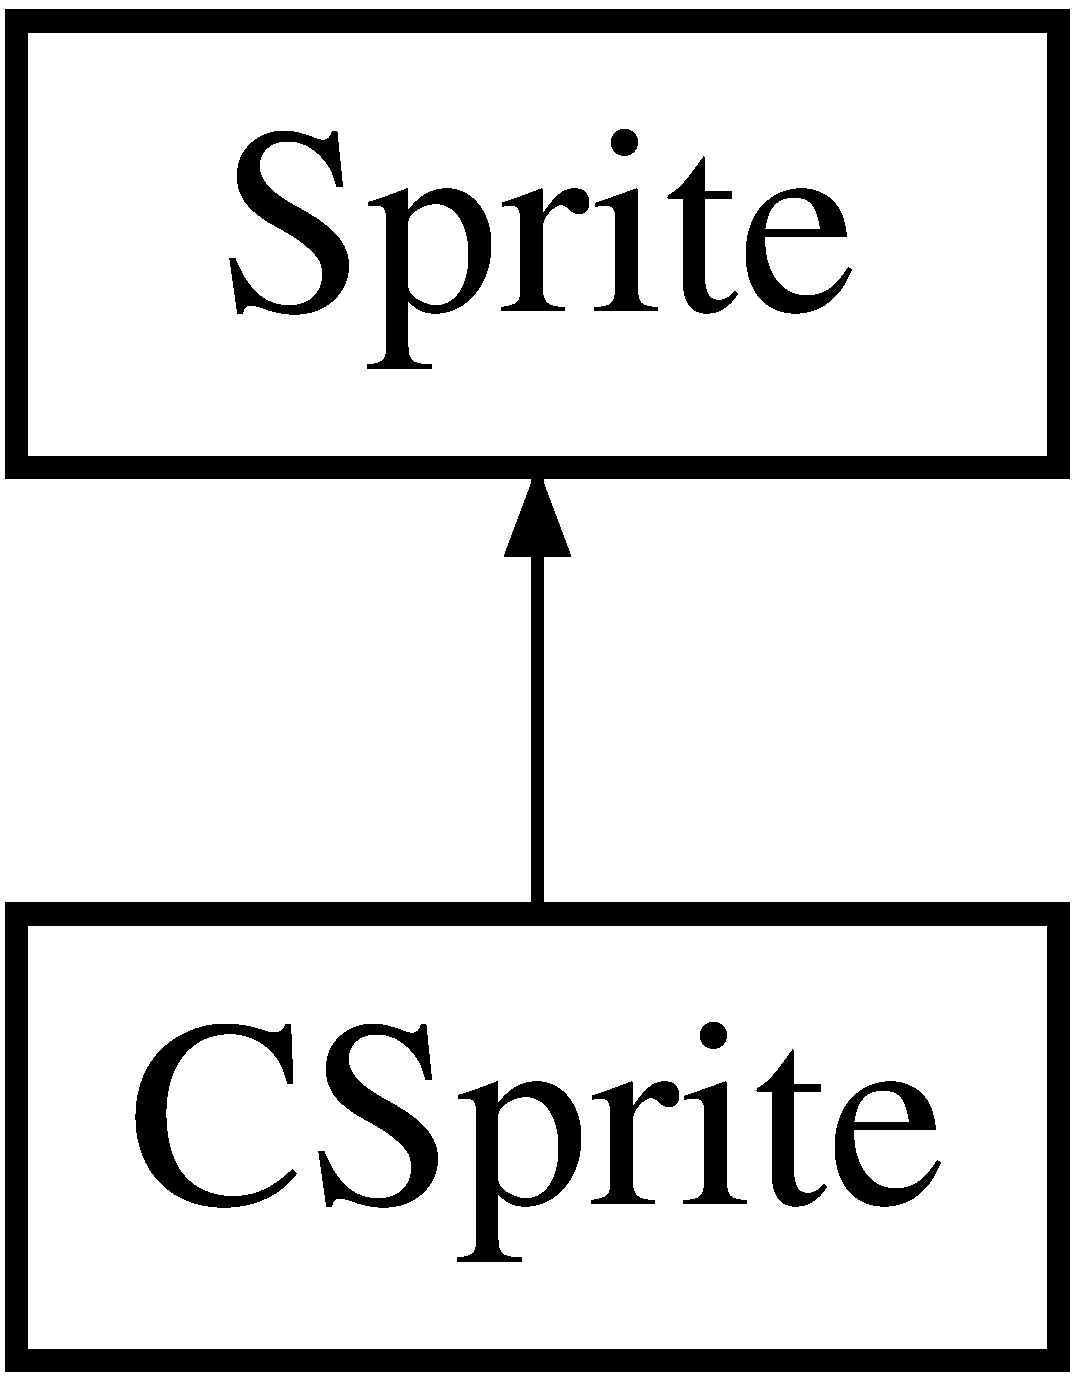
\includegraphics[height=2.000000cm]{classCSprite}
\end{center}
\end{figure}
\subsection*{Public Member Functions}
\begin{DoxyCompactItemize}
\item 
\hyperlink{classCSprite_afdfe7ac25b872dbafd60e6329185b0c5}{C\-Sprite} (\hyperlink{classCTexture}{C\-Texture} $\ast$p\-Texture, const sf\-::\-Vector2$<$ int $>$ \&curr\-Sub)
\item 
\hypertarget{classCSprite_a7fa10fe45cf1683163671b7483ffc758}{{\bfseries C\-Sprite} (const \hyperlink{classCSprite}{C\-Sprite} \&other)}\label{classCSprite_a7fa10fe45cf1683163671b7483ffc758}

\item 
\hypertarget{classCSprite_a2162a3b87f87eecf9e9b93fe4c573690}{void \hyperlink{classCSprite_a2162a3b87f87eecf9e9b93fe4c573690}{set\-Sub\-Image} (int col, int row)}\label{classCSprite_a2162a3b87f87eecf9e9b93fe4c573690}

\begin{DoxyCompactList}\small\item\em sets the current sub image being rendered from the texture \end{DoxyCompactList}\item 
\hypertarget{classCSprite_a6e46dd766754438ebdefadf3449540da}{void {\bfseries set\-Sub\-Image} (const sf\-::\-Vector2$<$ int $>$ $\ast$new\-Sub)}\label{classCSprite_a6e46dd766754438ebdefadf3449540da}

\end{DoxyCompactItemize}


\subsection{Detailed Description}


Definition at line 14 of file C\-Sprite.\-h.



\subsection{Constructor \& Destructor Documentation}
\hypertarget{classCSprite_afdfe7ac25b872dbafd60e6329185b0c5}{\index{C\-Sprite@{C\-Sprite}!C\-Sprite@{C\-Sprite}}
\index{C\-Sprite@{C\-Sprite}!CSprite@{C\-Sprite}}
\subsubsection[{C\-Sprite}]{\setlength{\rightskip}{0pt plus 5cm}C\-Sprite\-::\-C\-Sprite (
\begin{DoxyParamCaption}
\item[{{\bf C\-Texture} $\ast$}]{p\-Texture, }
\item[{const sf\-::\-Vector2$<$ int $>$ \&}]{curr\-Sub}
\end{DoxyParamCaption}
)}}\label{classCSprite_afdfe7ac25b872dbafd60e6329185b0c5}

\begin{DoxyParams}{Parameters}
{\em p\-Texture} & texture that this sprite will be rendering with \\
\hline
{\em curr\-Sub} & L\-E\-N\-G\-T\-H current sub-\/image being rendered \\
\hline
\end{DoxyParams}


Definition at line 13 of file C\-Sprite.\-cpp.



The documentation for this class was generated from the following files\-:\begin{DoxyCompactItemize}
\item 
/home/z\-Zelman/\-Dropbox/\-Covert-\/\-Collisions Host dir/\-Covert-\/\-Collisions/src/\-Headers/C\-Sprite.\-h\item 
/home/z\-Zelman/\-Dropbox/\-Covert-\/\-Collisions Host dir/\-Covert-\/\-Collisions/src/\-Graphics/C\-Sprite.\-cpp\end{DoxyCompactItemize}

\hypertarget{classCTexture}{\section{C\-Texture Class Reference}
\label{classCTexture}\index{C\-Texture@{C\-Texture}}
}


Wrapper class for S\-F\-M\-L 2.\-1 Texture.  




{\ttfamily \#include $<$C\-Texture.\-h$>$}



Inheritance diagram for C\-Texture\-:\nopagebreak
\begin{figure}[H]
\begin{center}
\leavevmode
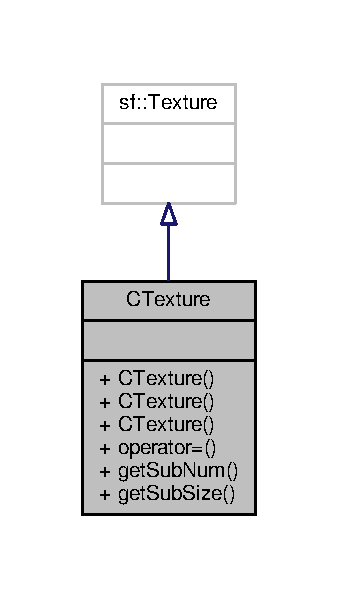
\includegraphics[width=162pt]{classCTexture__inherit__graph}
\end{center}
\end{figure}


Collaboration diagram for C\-Texture\-:\nopagebreak
\begin{figure}[H]
\begin{center}
\leavevmode
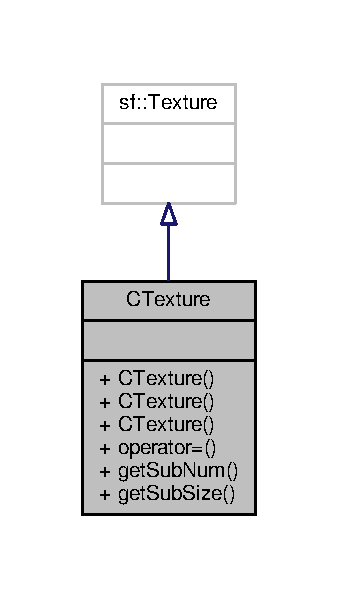
\includegraphics[width=162pt]{classCTexture__coll__graph}
\end{center}
\end{figure}
\subsection*{Public Member Functions}
\begin{DoxyCompactItemize}
\item 
\hyperlink{classCTexture_a4edabcc9e27ef0da135962c3490ec631}{C\-Texture} ()
\item 
\hyperlink{classCTexture_a03a03314b328783682d200443b561890}{C\-Texture} (std\-::string file\-Name, const sf\-::\-Vector2$<$ int $>$ \&sub\-Size, const sf\-::\-Vector2$<$ int $>$ \&sub\-Num)
\item 
\hyperlink{classCTexture_a2bb6709e0d63ccb6fb3219eb5528570f}{C\-Texture} (const \hyperlink{classCTexture}{C\-Texture} \&other)
\item 
\hyperlink{classCTexture}{C\-Texture} \& \hyperlink{classCTexture_ab4f29f7f73e347dfac33672e3b9a64c8}{operator=} (const \hyperlink{classCTexture}{C\-Texture} \&other)
\item 
const sf\-::\-Vector2$<$ int $>$ \& \hyperlink{classCTexture_a52a074211eaa812a91200f73f8387aca}{get\-Sub\-Num} () const 
\begin{DoxyCompactList}\small\item\em L\-E\-N\-G\-T\-H number of sub-\/section images on the full texture. \end{DoxyCompactList}\item 
const sf\-::\-Vector2$<$ int $>$ \& \hyperlink{classCTexture_a100f28379f113485d1e7574705ba977f}{get\-Sub\-Size} () const 
\begin{DoxyCompactList}\small\item\em L\-E\-N\-G\-T\-H of the sub-\/section image on the texture. \end{DoxyCompactList}\end{DoxyCompactItemize}


\subsection{Detailed Description}
Wrapper class for S\-F\-M\-L 2.\-1 Texture. 

Definition at line 16 of file C\-Texture.\-h.



\subsection{Constructor \& Destructor Documentation}
\hypertarget{classCTexture_a4edabcc9e27ef0da135962c3490ec631}{\index{C\-Texture@{C\-Texture}!C\-Texture@{C\-Texture}}
\index{C\-Texture@{C\-Texture}!CTexture@{C\-Texture}}
\subsubsection[{C\-Texture}]{\setlength{\rightskip}{0pt plus 5cm}C\-Texture\-::\-C\-Texture (
\begin{DoxyParamCaption}
{}
\end{DoxyParamCaption}
)}}\label{classCTexture_a4edabcc9e27ef0da135962c3490ec631}


Definition at line 13 of file C\-Texture.\-cpp.

\hypertarget{classCTexture_a03a03314b328783682d200443b561890}{\index{C\-Texture@{C\-Texture}!C\-Texture@{C\-Texture}}
\index{C\-Texture@{C\-Texture}!CTexture@{C\-Texture}}
\subsubsection[{C\-Texture}]{\setlength{\rightskip}{0pt plus 5cm}C\-Texture\-::\-C\-Texture (
\begin{DoxyParamCaption}
\item[{std\-::string}]{file\-Name, }
\item[{const sf\-::\-Vector2$<$ int $>$ \&}]{sub\-Size, }
\item[{const sf\-::\-Vector2$<$ int $>$ \&}]{sub\-Num}
\end{DoxyParamCaption}
)}}\label{classCTexture_a03a03314b328783682d200443b561890}

\begin{DoxyParams}{Parameters}
{\em file\-Name} & Relative full path to the texture image \\
\hline
{\em sub\-Size} & L\-E\-N\-G\-T\-H sub-\/image (x = width, y = height) \\
\hline
{\em sub\-Num} & L\-E\-N\-G\-T\-H number of sub images on the texture image \\
\hline
\end{DoxyParams}


Definition at line 19 of file C\-Texture.\-cpp.

\hypertarget{classCTexture_a2bb6709e0d63ccb6fb3219eb5528570f}{\index{C\-Texture@{C\-Texture}!C\-Texture@{C\-Texture}}
\index{C\-Texture@{C\-Texture}!CTexture@{C\-Texture}}
\subsubsection[{C\-Texture}]{\setlength{\rightskip}{0pt plus 5cm}C\-Texture\-::\-C\-Texture (
\begin{DoxyParamCaption}
\item[{const {\bf C\-Texture} \&}]{other}
\end{DoxyParamCaption}
)}}\label{classCTexture_a2bb6709e0d63ccb6fb3219eb5528570f}


Definition at line 31 of file C\-Texture.\-cpp.



\subsection{Member Function Documentation}
\hypertarget{classCTexture_a52a074211eaa812a91200f73f8387aca}{\index{C\-Texture@{C\-Texture}!get\-Sub\-Num@{get\-Sub\-Num}}
\index{get\-Sub\-Num@{get\-Sub\-Num}!CTexture@{C\-Texture}}
\subsubsection[{get\-Sub\-Num}]{\setlength{\rightskip}{0pt plus 5cm}const sf\-::\-Vector2$<$ int $>$ \& C\-Texture\-::get\-Sub\-Num (
\begin{DoxyParamCaption}
{}
\end{DoxyParamCaption}
) const}}\label{classCTexture_a52a074211eaa812a91200f73f8387aca}


L\-E\-N\-G\-T\-H number of sub-\/section images on the full texture. 

x = cols; y = rows 

Definition at line 56 of file C\-Texture.\-cpp.

\hypertarget{classCTexture_a100f28379f113485d1e7574705ba977f}{\index{C\-Texture@{C\-Texture}!get\-Sub\-Size@{get\-Sub\-Size}}
\index{get\-Sub\-Size@{get\-Sub\-Size}!CTexture@{C\-Texture}}
\subsubsection[{get\-Sub\-Size}]{\setlength{\rightskip}{0pt plus 5cm}const sf\-::\-Vector2$<$ int $>$ \& C\-Texture\-::get\-Sub\-Size (
\begin{DoxyParamCaption}
{}
\end{DoxyParamCaption}
) const}}\label{classCTexture_a100f28379f113485d1e7574705ba977f}


L\-E\-N\-G\-T\-H of the sub-\/section image on the texture. 

x = width; y = height 

Definition at line 62 of file C\-Texture.\-cpp.

\hypertarget{classCTexture_ab4f29f7f73e347dfac33672e3b9a64c8}{\index{C\-Texture@{C\-Texture}!operator=@{operator=}}
\index{operator=@{operator=}!CTexture@{C\-Texture}}
\subsubsection[{operator=}]{\setlength{\rightskip}{0pt plus 5cm}{\bf C\-Texture} \& C\-Texture\-::operator= (
\begin{DoxyParamCaption}
\item[{const {\bf C\-Texture} \&}]{other}
\end{DoxyParamCaption}
)}}\label{classCTexture_ab4f29f7f73e347dfac33672e3b9a64c8}


Definition at line 39 of file C\-Texture.\-cpp.



The documentation for this class was generated from the following files\-:\begin{DoxyCompactItemize}
\item 
/home/z\-Zelman/\-Dropbox/\-Covert-\/\-Collisions Host dir/\-Covert-\/\-Collisions/src/\-Headers/\hyperlink{CTexture_8h}{C\-Texture.\-h}\item 
/home/z\-Zelman/\-Dropbox/\-Covert-\/\-Collisions Host dir/\-Covert-\/\-Collisions/src/\-Graphics/\hyperlink{CTexture_8cpp}{C\-Texture.\-cpp}\end{DoxyCompactItemize}

\hypertarget{classCTile}{\section{C\-Tile Class Reference}
\label{classCTile}\index{C\-Tile@{C\-Tile}}
}
Inheritance diagram for C\-Tile\-:\begin{figure}[H]
\begin{center}
\leavevmode
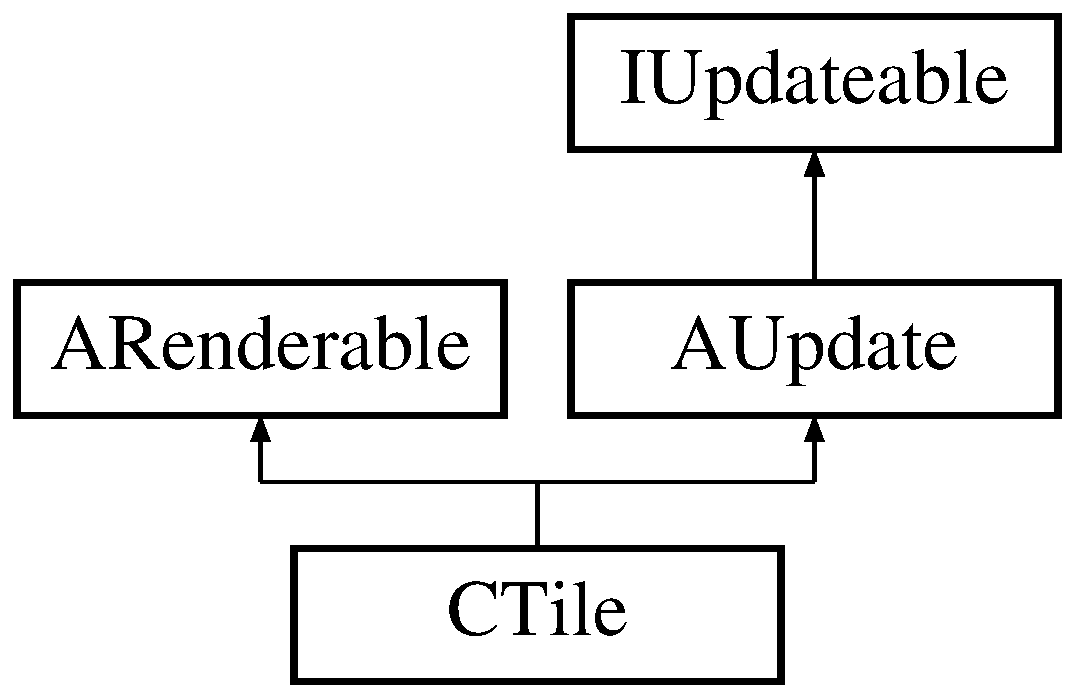
\includegraphics[height=3.000000cm]{classCTile}
\end{center}
\end{figure}
\subsection*{Public Member Functions}
\begin{DoxyCompactItemize}
\item 
\hypertarget{classCTile_a030eef2d18fb054c0fa6738784af0b0d}{{\bfseries C\-Tile} (\hyperlink{classCTexture}{C\-Texture} $\ast$p\-Texture, const sf\-::\-Vector2$<$ int $>$ \&curr\-Sub)}\label{classCTile_a030eef2d18fb054c0fa6738784af0b0d}

\item 
\hypertarget{classCTile_a07c38be9c331480eb7c8d526b084a287}{{\bfseries C\-Tile} (\hyperlink{classCSprite}{C\-Sprite} $\ast$p\-Sprite)}\label{classCTile_a07c38be9c331480eb7c8d526b084a287}

\item 
\hypertarget{classCTile_a818a17e48a7219eedac950b82c641ee0}{void {\bfseries update} ()}\label{classCTile_a818a17e48a7219eedac950b82c641ee0}

\end{DoxyCompactItemize}
\subsection*{Additional Inherited Members}


\subsection{Detailed Description}


Definition at line 16 of file C\-Tile.\-h.



The documentation for this class was generated from the following files\-:\begin{DoxyCompactItemize}
\item 
/home/z\-Zelman/\-Dropbox/\-Covert-\/\-Collisions Host dir/\-Covert-\/\-Collisions/src/\-Headers/C\-Tile.\-h\item 
/home/z\-Zelman/\-Dropbox/\-Covert-\/\-Collisions Host dir/\-Covert-\/\-Collisions/src/\-Tiles/C\-Tile.\-cpp\end{DoxyCompactItemize}

\hypertarget{classCTile__Container}{\section{C\-Tile\-\_\-\-Container Class Reference}
\label{classCTile__Container}\index{C\-Tile\-\_\-\-Container@{C\-Tile\-\_\-\-Container}}
}


T\-O\-D\-O\-: This object needs to be re-\/writen to expand functionality.  




{\ttfamily \#include $<$C\-Tile\-\_\-\-Container.\-h$>$}



Inheritance diagram for C\-Tile\-\_\-\-Container\-:\nopagebreak
\begin{figure}[H]
\begin{center}
\leavevmode
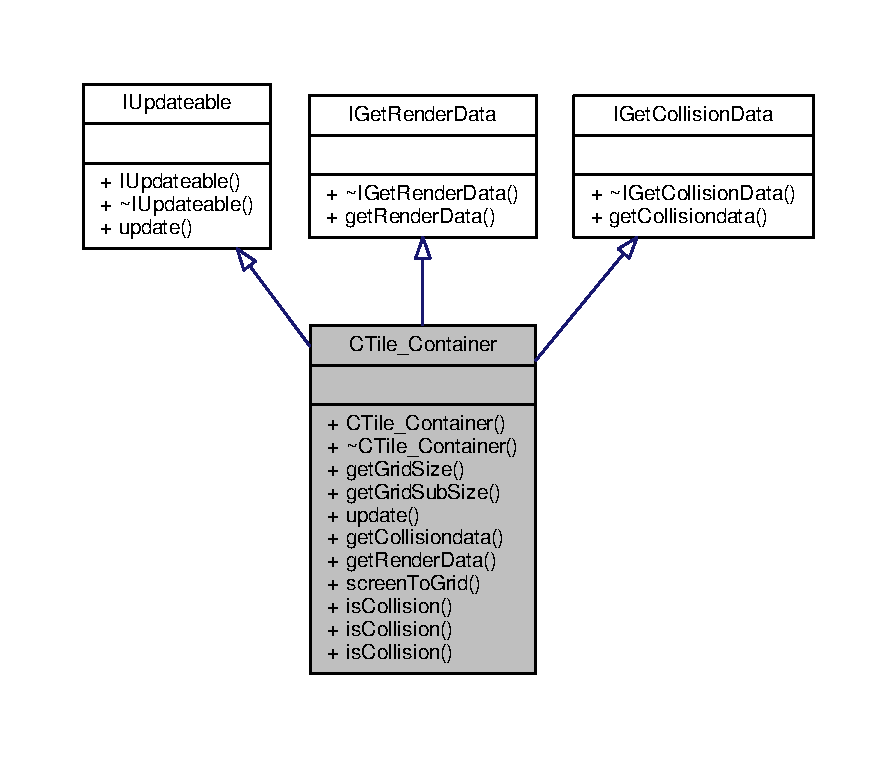
\includegraphics[width=350pt]{classCTile__Container__inherit__graph}
\end{center}
\end{figure}


Collaboration diagram for C\-Tile\-\_\-\-Container\-:\nopagebreak
\begin{figure}[H]
\begin{center}
\leavevmode
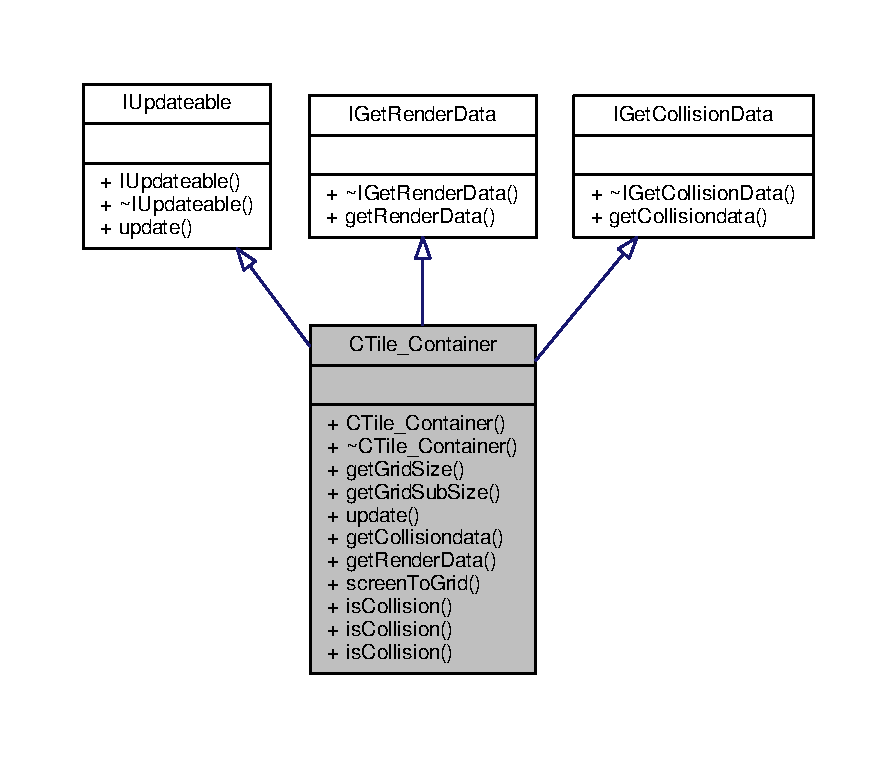
\includegraphics[width=350pt]{classCTile__Container__coll__graph}
\end{center}
\end{figure}
\subsection*{Public Member Functions}
\begin{DoxyCompactItemize}
\item 
\hyperlink{classCTile__Container_ab3f79e82961b644d422874eb558ea312}{C\-Tile\-\_\-\-Container} (std\-::string file\-Name)
\item 
\hyperlink{classCTile__Container_ac62ffead3e87a0c405d7bd6f25581927}{$\sim$\-C\-Tile\-\_\-\-Container} ()
\item 
sf\-::\-Vector2$<$ int $>$ \hyperlink{classCTile__Container_ae8a4d2b6e49fbec47d92cbb19bb9d3c7}{get\-Grid\-Size} ()
\item 
sf\-::\-Vector2$<$ int $>$ \hyperlink{classCTile__Container_a876984278369d0cafc24890959128ed0}{get\-Grid\-Sub\-Size} ()
\item 
void \hyperlink{classCTile__Container_abe6e19de544f042671094697bb83fde9}{update} ()
\item 
void \hyperlink{classCTile__Container_ae61b573ed7b47bea750040a26b492632}{get\-Collisiondata} (std\-::list$<$ \hyperlink{classARenderable}{A\-Renderable} $\ast$ $>$ $\ast$p\-List)
\begin{DoxyCompactList}\small\item\em All objects that implement this interface agree to allow their pointers to Derived Classes of A\-Render to be placed within the given std\-::list so that they may be used for quad-\/tree collision detection. \end{DoxyCompactList}\item 
void \hyperlink{classCTile__Container_a48c74611efadee522595362a79620bff}{get\-Render\-Data} (std\-::list$<$ \hyperlink{classARenderable}{A\-Renderable} $\ast$ $>$ $\ast$p\-List)
\begin{DoxyCompactList}\small\item\em Fills the std\-::list with objects that need to be rendered. \end{DoxyCompactList}\item 
void \hyperlink{classCTile__Container_a14f90644c3a992813a629cea3e81aa38}{screen\-To\-Grid} (int $\ast$pos\-X, int $\ast$pos\-Y)
\item 
bool \hyperlink{classCTile__Container_adfda15836508531632c4ca506caf6360}{is\-Collision} (const sf\-::\-Rect$<$ float $>$ \&rect, \hyperlink{classCSprite}{C\-Sprite} $\ast$\&p\-Sprite)
\item 
bool \hyperlink{classCTile__Container_a4195d75fcc4790946b19ea82fc693a1c}{is\-Collision} (const sf\-::\-Vector2$<$ float $>$ \&point, \hyperlink{classCSprite}{C\-Sprite} $\ast$\&p\-Sprite)
\item 
bool \hyperlink{classCTile__Container_a3c8b4ccbb9afaaa9462a11962b6e2dbd}{is\-Collision} (float x, float y, \hyperlink{classCSprite}{C\-Sprite} $\ast$\&p\-Sprite)
\end{DoxyCompactItemize}


\subsection{Detailed Description}
T\-O\-D\-O\-: This object needs to be re-\/writen to expand functionality. 

Custom Container for holding individual \hyperlink{classCTile}{C\-Tile}.

\begin{DoxySeeAlso}{See Also}
\hyperlink{classCTile}{C\-Tile} 
\end{DoxySeeAlso}


Definition at line 30 of file C\-Tile\-\_\-\-Container.\-h.



\subsection{Constructor \& Destructor Documentation}
\hypertarget{classCTile__Container_ab3f79e82961b644d422874eb558ea312}{\index{C\-Tile\-\_\-\-Container@{C\-Tile\-\_\-\-Container}!C\-Tile\-\_\-\-Container@{C\-Tile\-\_\-\-Container}}
\index{C\-Tile\-\_\-\-Container@{C\-Tile\-\_\-\-Container}!CTile_Container@{C\-Tile\-\_\-\-Container}}
\subsubsection[{C\-Tile\-\_\-\-Container}]{\setlength{\rightskip}{0pt plus 5cm}C\-Tile\-\_\-\-Container\-::\-C\-Tile\-\_\-\-Container (
\begin{DoxyParamCaption}
\item[{std\-::string}]{file\-Name}
\end{DoxyParamCaption}
)}}\label{classCTile__Container_ab3f79e82961b644d422874eb558ea312}


Definition at line 19 of file C\-Tile\-\_\-\-Container.\-cpp.

\hypertarget{classCTile__Container_ac62ffead3e87a0c405d7bd6f25581927}{\index{C\-Tile\-\_\-\-Container@{C\-Tile\-\_\-\-Container}!$\sim$\-C\-Tile\-\_\-\-Container@{$\sim$\-C\-Tile\-\_\-\-Container}}
\index{$\sim$\-C\-Tile\-\_\-\-Container@{$\sim$\-C\-Tile\-\_\-\-Container}!CTile_Container@{C\-Tile\-\_\-\-Container}}
\subsubsection[{$\sim$\-C\-Tile\-\_\-\-Container}]{\setlength{\rightskip}{0pt plus 5cm}C\-Tile\-\_\-\-Container\-::$\sim$\-C\-Tile\-\_\-\-Container (
\begin{DoxyParamCaption}
{}
\end{DoxyParamCaption}
)}}\label{classCTile__Container_ac62ffead3e87a0c405d7bd6f25581927}


Definition at line 32 of file C\-Tile\-\_\-\-Container.\-cpp.



\subsection{Member Function Documentation}
\hypertarget{classCTile__Container_ae61b573ed7b47bea750040a26b492632}{\index{C\-Tile\-\_\-\-Container@{C\-Tile\-\_\-\-Container}!get\-Collisiondata@{get\-Collisiondata}}
\index{get\-Collisiondata@{get\-Collisiondata}!CTile_Container@{C\-Tile\-\_\-\-Container}}
\subsubsection[{get\-Collisiondata}]{\setlength{\rightskip}{0pt plus 5cm}void C\-Tile\-\_\-\-Container\-::get\-Collisiondata (
\begin{DoxyParamCaption}
\item[{std\-::list$<$ {\bf A\-Renderable} $\ast$ $>$ $\ast$}]{p\-List}
\end{DoxyParamCaption}
)\hspace{0.3cm}{\ttfamily [virtual]}}}\label{classCTile__Container_ae61b573ed7b47bea750040a26b492632}


All objects that implement this interface agree to allow their pointers to Derived Classes of A\-Render to be placed within the given std\-::list so that they may be used for quad-\/tree collision detection. 



Implements \hyperlink{classIGetCollisionData_ad31b95dda265659e5090fc2c188b30b9}{I\-Get\-Collision\-Data}.



Definition at line 75 of file C\-Tile\-\_\-\-Container.\-cpp.

\hypertarget{classCTile__Container_ae8a4d2b6e49fbec47d92cbb19bb9d3c7}{\index{C\-Tile\-\_\-\-Container@{C\-Tile\-\_\-\-Container}!get\-Grid\-Size@{get\-Grid\-Size}}
\index{get\-Grid\-Size@{get\-Grid\-Size}!CTile_Container@{C\-Tile\-\_\-\-Container}}
\subsubsection[{get\-Grid\-Size}]{\setlength{\rightskip}{0pt plus 5cm}sf\-::\-Vector2$<$ int $>$ C\-Tile\-\_\-\-Container\-::get\-Grid\-Size (
\begin{DoxyParamCaption}
{}
\end{DoxyParamCaption}
)}}\label{classCTile__Container_ae8a4d2b6e49fbec47d92cbb19bb9d3c7}


Definition at line 47 of file C\-Tile\-\_\-\-Container.\-cpp.

\hypertarget{classCTile__Container_a876984278369d0cafc24890959128ed0}{\index{C\-Tile\-\_\-\-Container@{C\-Tile\-\_\-\-Container}!get\-Grid\-Sub\-Size@{get\-Grid\-Sub\-Size}}
\index{get\-Grid\-Sub\-Size@{get\-Grid\-Sub\-Size}!CTile_Container@{C\-Tile\-\_\-\-Container}}
\subsubsection[{get\-Grid\-Sub\-Size}]{\setlength{\rightskip}{0pt plus 5cm}sf\-::\-Vector2$<$ int $>$ C\-Tile\-\_\-\-Container\-::get\-Grid\-Sub\-Size (
\begin{DoxyParamCaption}
{}
\end{DoxyParamCaption}
)}}\label{classCTile__Container_a876984278369d0cafc24890959128ed0}


Definition at line 53 of file C\-Tile\-\_\-\-Container.\-cpp.

\hypertarget{classCTile__Container_a48c74611efadee522595362a79620bff}{\index{C\-Tile\-\_\-\-Container@{C\-Tile\-\_\-\-Container}!get\-Render\-Data@{get\-Render\-Data}}
\index{get\-Render\-Data@{get\-Render\-Data}!CTile_Container@{C\-Tile\-\_\-\-Container}}
\subsubsection[{get\-Render\-Data}]{\setlength{\rightskip}{0pt plus 5cm}void C\-Tile\-\_\-\-Container\-::get\-Render\-Data (
\begin{DoxyParamCaption}
\item[{std\-::list$<$ {\bf A\-Renderable} $\ast$ $>$ $\ast$}]{p\-List}
\end{DoxyParamCaption}
)\hspace{0.3cm}{\ttfamily [virtual]}}}\label{classCTile__Container_a48c74611efadee522595362a79620bff}


Fills the std\-::list with objects that need to be rendered. 



Implements \hyperlink{classIGetRenderData_ac98527f07b6d1b5030786b4848cca867}{I\-Get\-Render\-Data}.



Definition at line 64 of file C\-Tile\-\_\-\-Container.\-cpp.

\hypertarget{classCTile__Container_adfda15836508531632c4ca506caf6360}{\index{C\-Tile\-\_\-\-Container@{C\-Tile\-\_\-\-Container}!is\-Collision@{is\-Collision}}
\index{is\-Collision@{is\-Collision}!CTile_Container@{C\-Tile\-\_\-\-Container}}
\subsubsection[{is\-Collision}]{\setlength{\rightskip}{0pt plus 5cm}bool C\-Tile\-\_\-\-Container\-::is\-Collision (
\begin{DoxyParamCaption}
\item[{const sf\-::\-Rect$<$ float $>$ \&}]{rect, }
\item[{{\bf C\-Sprite} $\ast$\&}]{p\-Sprite}
\end{DoxyParamCaption}
)}}\label{classCTile__Container_adfda15836508531632c4ca506caf6360}


Definition at line 102 of file C\-Tile\-\_\-\-Container.\-cpp.

\hypertarget{classCTile__Container_a4195d75fcc4790946b19ea82fc693a1c}{\index{C\-Tile\-\_\-\-Container@{C\-Tile\-\_\-\-Container}!is\-Collision@{is\-Collision}}
\index{is\-Collision@{is\-Collision}!CTile_Container@{C\-Tile\-\_\-\-Container}}
\subsubsection[{is\-Collision}]{\setlength{\rightskip}{0pt plus 5cm}bool C\-Tile\-\_\-\-Container\-::is\-Collision (
\begin{DoxyParamCaption}
\item[{const sf\-::\-Vector2$<$ float $>$ \&}]{point, }
\item[{{\bf C\-Sprite} $\ast$\&}]{p\-Sprite}
\end{DoxyParamCaption}
)}}\label{classCTile__Container_a4195d75fcc4790946b19ea82fc693a1c}


Definition at line 124 of file C\-Tile\-\_\-\-Container.\-cpp.

\hypertarget{classCTile__Container_a3c8b4ccbb9afaaa9462a11962b6e2dbd}{\index{C\-Tile\-\_\-\-Container@{C\-Tile\-\_\-\-Container}!is\-Collision@{is\-Collision}}
\index{is\-Collision@{is\-Collision}!CTile_Container@{C\-Tile\-\_\-\-Container}}
\subsubsection[{is\-Collision}]{\setlength{\rightskip}{0pt plus 5cm}bool C\-Tile\-\_\-\-Container\-::is\-Collision (
\begin{DoxyParamCaption}
\item[{float}]{x, }
\item[{float}]{y, }
\item[{{\bf C\-Sprite} $\ast$\&}]{p\-Sprite}
\end{DoxyParamCaption}
)}}\label{classCTile__Container_a3c8b4ccbb9afaaa9462a11962b6e2dbd}


Definition at line 130 of file C\-Tile\-\_\-\-Container.\-cpp.

\hypertarget{classCTile__Container_a14f90644c3a992813a629cea3e81aa38}{\index{C\-Tile\-\_\-\-Container@{C\-Tile\-\_\-\-Container}!screen\-To\-Grid@{screen\-To\-Grid}}
\index{screen\-To\-Grid@{screen\-To\-Grid}!CTile_Container@{C\-Tile\-\_\-\-Container}}
\subsubsection[{screen\-To\-Grid}]{\setlength{\rightskip}{0pt plus 5cm}void C\-Tile\-\_\-\-Container\-::screen\-To\-Grid (
\begin{DoxyParamCaption}
\item[{int $\ast$}]{pos\-X, }
\item[{int $\ast$}]{pos\-Y}
\end{DoxyParamCaption}
)}}\label{classCTile__Container_a14f90644c3a992813a629cea3e81aa38}


Definition at line 86 of file C\-Tile\-\_\-\-Container.\-cpp.

\hypertarget{classCTile__Container_abe6e19de544f042671094697bb83fde9}{\index{C\-Tile\-\_\-\-Container@{C\-Tile\-\_\-\-Container}!update@{update}}
\index{update@{update}!CTile_Container@{C\-Tile\-\_\-\-Container}}
\subsubsection[{update}]{\setlength{\rightskip}{0pt plus 5cm}void C\-Tile\-\_\-\-Container\-::update (
\begin{DoxyParamCaption}
{}
\end{DoxyParamCaption}
)\hspace{0.3cm}{\ttfamily [virtual]}}}\label{classCTile__Container_abe6e19de544f042671094697bb83fde9}


Implements \hyperlink{classIUpdateable_a46d178a1ecdab33bcaad25d9b38582a5}{I\-Updateable}.



Definition at line 59 of file C\-Tile\-\_\-\-Container.\-cpp.



The documentation for this class was generated from the following files\-:\begin{DoxyCompactItemize}
\item 
/home/z\-Zelman/\-Dropbox/\-Covert-\/\-Collisions Host dir/\-Covert-\/\-Collisions/src/\-Headers/\hyperlink{CTile__Container_8h}{C\-Tile\-\_\-\-Container.\-h}\item 
/home/z\-Zelman/\-Dropbox/\-Covert-\/\-Collisions Host dir/\-Covert-\/\-Collisions/src/\-Tiles/\hyperlink{CTile__Container_8cpp}{C\-Tile\-\_\-\-Container.\-cpp}\end{DoxyCompactItemize}

\hypertarget{classCUI}{\section{C\-U\-I Class Reference}
\label{classCUI}\index{C\-U\-I@{C\-U\-I}}
}


'Parses' user events, as well as keeps Bookkeeping information on several user states.  




{\ttfamily \#include $<$C\-U\-I.\-h$>$}



Inheritance diagram for C\-U\-I\-:
\nopagebreak
\begin{figure}[H]
\begin{center}
\leavevmode
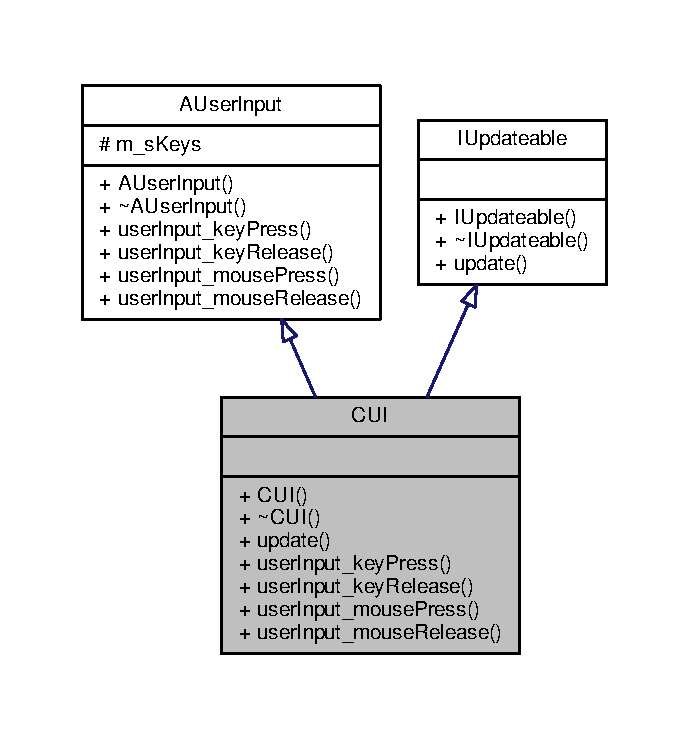
\includegraphics[width=331pt]{classCUI__inherit__graph}
\end{center}
\end{figure}


Collaboration diagram for C\-U\-I\-:
\nopagebreak
\begin{figure}[H]
\begin{center}
\leavevmode
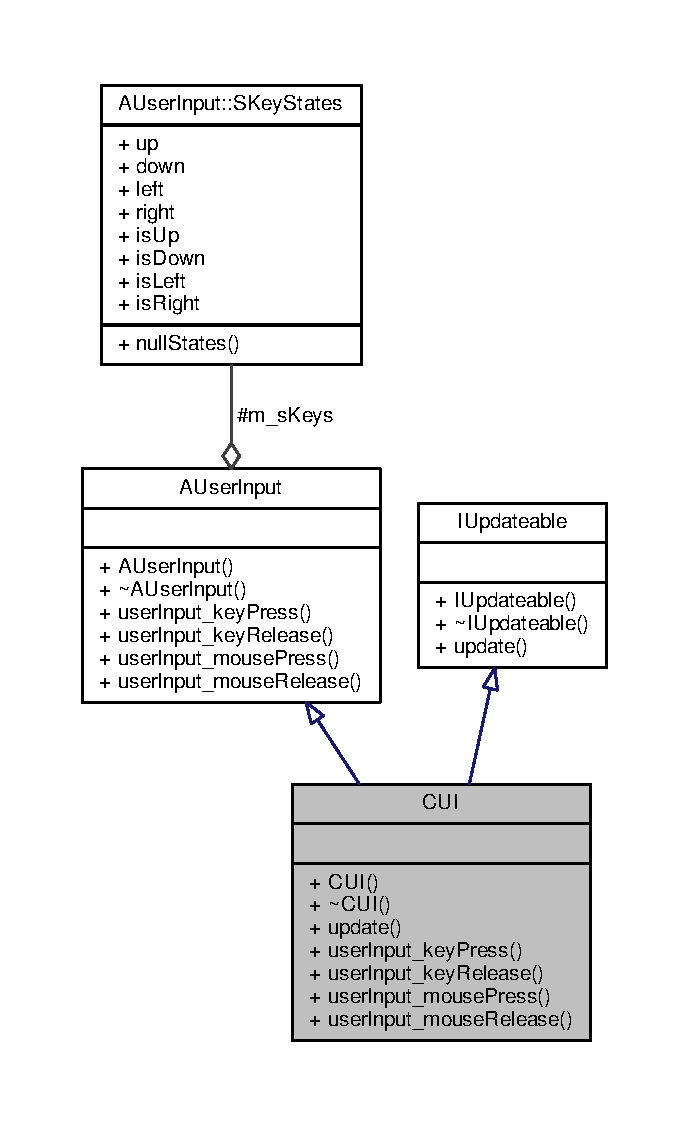
\includegraphics[width=331pt]{classCUI__coll__graph}
\end{center}
\end{figure}
\subsection*{Public Member Functions}
\begin{DoxyCompactItemize}
\item 
\hyperlink{classCUI_aaca9bcb98d25fa4b4868bc3266f44ec6}{C\-U\-I} (\hyperlink{classCPlayer}{C\-Player} $\ast$p\-Player)
\item 
\hyperlink{classCUI_a76a9c9d894e90c77549c4393c1181598}{$\sim$\-C\-U\-I} ()
\item 
void \hyperlink{classCUI_ab0b322040b41a6650bd625216f77b75c}{update} ()
\item 
bool \hyperlink{classCUI_addb1531f20541cb7c7f8688f1cd843e9}{user\-Input\-\_\-key\-Press} (sf\-::\-Event $\ast$p\-Event)
\item 
bool \hyperlink{classCUI_a0495bb6ad5fba9ef0552a487151f7896}{user\-Input\-\_\-key\-Release} (sf\-::\-Event $\ast$p\-Event)
\item 
bool \hyperlink{classCUI_a6edfa48bb429f6e1468f5c3568cf83c5}{user\-Input\-\_\-mouse\-Press} (sf\-::\-Event $\ast$p\-Event)
\item 
bool \hyperlink{classCUI_a64e3c8ad256e2d814e7112d201cb78ae}{user\-Input\-\_\-mouse\-Release} (sf\-::\-Event $\ast$p\-Event)
\end{DoxyCompactItemize}
\subsection*{Additional Inherited Members}


\subsection{Detailed Description}
'Parses' user events, as well as keeps Bookkeeping information on several user states. 

T\-O\-D\-O\-: Uses a finite state machine to determine how user events are interpreted (menu vs. game-\/play) 

Definition at line 23 of file C\-U\-I.\-h.



\subsection{Constructor \& Destructor Documentation}
\hypertarget{classCUI_aaca9bcb98d25fa4b4868bc3266f44ec6}{\index{C\-U\-I@{C\-U\-I}!C\-U\-I@{C\-U\-I}}
\index{C\-U\-I@{C\-U\-I}!CUI@{C\-U\-I}}
\subsubsection[{C\-U\-I}]{\setlength{\rightskip}{0pt plus 5cm}C\-U\-I\-::\-C\-U\-I (
\begin{DoxyParamCaption}
\item[{{\bf C\-Player} $\ast$}]{p\-Player}
\end{DoxyParamCaption}
)}}\label{classCUI_aaca9bcb98d25fa4b4868bc3266f44ec6}


Definition at line 12 of file C\-U\-I.\-cpp.

\hypertarget{classCUI_a76a9c9d894e90c77549c4393c1181598}{\index{C\-U\-I@{C\-U\-I}!$\sim$\-C\-U\-I@{$\sim$\-C\-U\-I}}
\index{$\sim$\-C\-U\-I@{$\sim$\-C\-U\-I}!CUI@{C\-U\-I}}
\subsubsection[{$\sim$\-C\-U\-I}]{\setlength{\rightskip}{0pt plus 5cm}C\-U\-I\-::$\sim$\-C\-U\-I (
\begin{DoxyParamCaption}
{}
\end{DoxyParamCaption}
)}}\label{classCUI_a76a9c9d894e90c77549c4393c1181598}


Definition at line 18 of file C\-U\-I.\-cpp.



\subsection{Member Function Documentation}
\hypertarget{classCUI_ab0b322040b41a6650bd625216f77b75c}{\index{C\-U\-I@{C\-U\-I}!update@{update}}
\index{update@{update}!CUI@{C\-U\-I}}
\subsubsection[{update}]{\setlength{\rightskip}{0pt plus 5cm}void C\-U\-I\-::update (
\begin{DoxyParamCaption}
{}
\end{DoxyParamCaption}
)\hspace{0.3cm}{\ttfamily [virtual]}}}\label{classCUI_ab0b322040b41a6650bd625216f77b75c}


Implements \hyperlink{classIUpdateable_a46d178a1ecdab33bcaad25d9b38582a5}{I\-Updateable}.



Definition at line 23 of file C\-U\-I.\-cpp.

\hypertarget{classCUI_addb1531f20541cb7c7f8688f1cd843e9}{\index{C\-U\-I@{C\-U\-I}!user\-Input\-\_\-key\-Press@{user\-Input\-\_\-key\-Press}}
\index{user\-Input\-\_\-key\-Press@{user\-Input\-\_\-key\-Press}!CUI@{C\-U\-I}}
\subsubsection[{user\-Input\-\_\-key\-Press}]{\setlength{\rightskip}{0pt plus 5cm}bool C\-U\-I\-::user\-Input\-\_\-key\-Press (
\begin{DoxyParamCaption}
\item[{sf\-::\-Event $\ast$}]{p\-Event}
\end{DoxyParamCaption}
)\hspace{0.3cm}{\ttfamily [virtual]}}}\label{classCUI_addb1531f20541cb7c7f8688f1cd843e9}


Implements \hyperlink{classAUserInput_a110239bcc0461666583d1dc940cb5d13}{A\-User\-Input}.



Definition at line 28 of file C\-U\-I.\-cpp.

\hypertarget{classCUI_a0495bb6ad5fba9ef0552a487151f7896}{\index{C\-U\-I@{C\-U\-I}!user\-Input\-\_\-key\-Release@{user\-Input\-\_\-key\-Release}}
\index{user\-Input\-\_\-key\-Release@{user\-Input\-\_\-key\-Release}!CUI@{C\-U\-I}}
\subsubsection[{user\-Input\-\_\-key\-Release}]{\setlength{\rightskip}{0pt plus 5cm}bool C\-U\-I\-::user\-Input\-\_\-key\-Release (
\begin{DoxyParamCaption}
\item[{sf\-::\-Event $\ast$}]{p\-Event}
\end{DoxyParamCaption}
)\hspace{0.3cm}{\ttfamily [virtual]}}}\label{classCUI_a0495bb6ad5fba9ef0552a487151f7896}


Implements \hyperlink{classAUserInput_afe8ae22fff673d788e366b9b29ffa67d}{A\-User\-Input}.



Definition at line 40 of file C\-U\-I.\-cpp.

\hypertarget{classCUI_a6edfa48bb429f6e1468f5c3568cf83c5}{\index{C\-U\-I@{C\-U\-I}!user\-Input\-\_\-mouse\-Press@{user\-Input\-\_\-mouse\-Press}}
\index{user\-Input\-\_\-mouse\-Press@{user\-Input\-\_\-mouse\-Press}!CUI@{C\-U\-I}}
\subsubsection[{user\-Input\-\_\-mouse\-Press}]{\setlength{\rightskip}{0pt plus 5cm}bool C\-U\-I\-::user\-Input\-\_\-mouse\-Press (
\begin{DoxyParamCaption}
\item[{sf\-::\-Event $\ast$}]{p\-Event}
\end{DoxyParamCaption}
)\hspace{0.3cm}{\ttfamily [virtual]}}}\label{classCUI_a6edfa48bb429f6e1468f5c3568cf83c5}


Implements \hyperlink{classAUserInput_a567e0d0610bd2ef2e23fed64b3e56d2b}{A\-User\-Input}.



Definition at line 53 of file C\-U\-I.\-cpp.

\hypertarget{classCUI_a64e3c8ad256e2d814e7112d201cb78ae}{\index{C\-U\-I@{C\-U\-I}!user\-Input\-\_\-mouse\-Release@{user\-Input\-\_\-mouse\-Release}}
\index{user\-Input\-\_\-mouse\-Release@{user\-Input\-\_\-mouse\-Release}!CUI@{C\-U\-I}}
\subsubsection[{user\-Input\-\_\-mouse\-Release}]{\setlength{\rightskip}{0pt plus 5cm}bool C\-U\-I\-::user\-Input\-\_\-mouse\-Release (
\begin{DoxyParamCaption}
\item[{sf\-::\-Event $\ast$}]{p\-Event}
\end{DoxyParamCaption}
)\hspace{0.3cm}{\ttfamily [virtual]}}}\label{classCUI_a64e3c8ad256e2d814e7112d201cb78ae}


Implements \hyperlink{classAUserInput_a570f71dde4825c3e9bdcf6b58857f514}{A\-User\-Input}.



Definition at line 67 of file C\-U\-I.\-cpp.



The documentation for this class was generated from the following files\-:\begin{DoxyCompactItemize}
\item 
/home/z\-Zelman/\-Dropbox/\-Covert-\/\-Collisions Host dir/\-Covert-\/\-Collisions/src/\-Headers/\hyperlink{CUI_8h}{C\-U\-I.\-h}\item 
/home/z\-Zelman/\-Dropbox/\-Covert-\/\-Collisions Host dir/\-Covert-\/\-Collisions/src/\-U\-I/\hyperlink{CUI_8cpp}{C\-U\-I.\-cpp}\end{DoxyCompactItemize}

\hypertarget{classDPhysics}{\section{D\-Physics Class Reference}
\label{classDPhysics}\index{D\-Physics@{D\-Physics}}
}


Base class holder of pertinent physics information within a \hyperlink{structDPhysics_1_1SPhysics}{S\-Physics}.  




{\ttfamily \#include $<$D\-Physics.\-h$>$}



Inheritance diagram for D\-Physics\-:\nopagebreak
\begin{figure}[H]
\begin{center}
\leavevmode
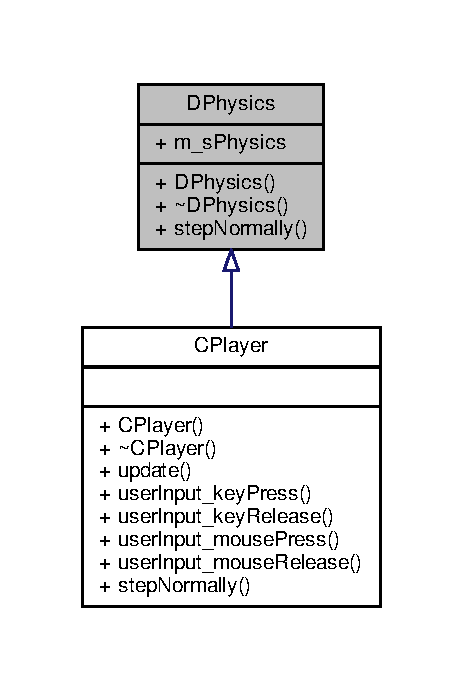
\includegraphics[width=222pt]{classDPhysics__inherit__graph}
\end{center}
\end{figure}


Collaboration diagram for D\-Physics\-:\nopagebreak
\begin{figure}[H]
\begin{center}
\leavevmode
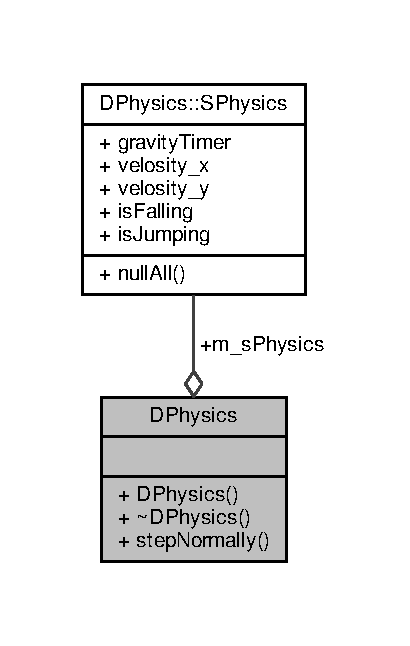
\includegraphics[width=197pt]{classDPhysics__coll__graph}
\end{center}
\end{figure}
\subsection*{Classes}
\begin{DoxyCompactItemize}
\item 
struct \hyperlink{structDPhysics_1_1SPhysics}{S\-Physics}
\begin{DoxyCompactList}\small\item\em Physics data. \end{DoxyCompactList}\end{DoxyCompactItemize}
\subsection*{Public Member Functions}
\begin{DoxyCompactItemize}
\item 
\hyperlink{classDPhysics_a3ce58ebc308881f3eb0cff60ff1eff45}{D\-Physics} ()
\item 
virtual \hyperlink{classDPhysics_aad555af54aca363984d0fcf34d044ba5}{$\sim$\-D\-Physics} ()
\item 
virtual void \hyperlink{classDPhysics_a414316ffcec06dbf01ced086bbb92b55}{step\-Normally} ()=0
\begin{DoxyCompactList}\small\item\em A normal step in 1 update call. \end{DoxyCompactList}\end{DoxyCompactItemize}
\subsection*{Public Attributes}
\begin{DoxyCompactItemize}
\item 
struct \hyperlink{structDPhysics_1_1SPhysics}{D\-Physics\-::\-S\-Physics} \hyperlink{classDPhysics_aca2940879481f0e2b892c82c5fc0da5a}{m\-\_\-s\-Physics}
\end{DoxyCompactItemize}


\subsection{Detailed Description}
Base class holder of pertinent physics information within a \hyperlink{structDPhysics_1_1SPhysics}{S\-Physics}. 

Definition at line 17 of file D\-Physics.\-h.



\subsection{Constructor \& Destructor Documentation}
\hypertarget{classDPhysics_a3ce58ebc308881f3eb0cff60ff1eff45}{\index{D\-Physics@{D\-Physics}!D\-Physics@{D\-Physics}}
\index{D\-Physics@{D\-Physics}!DPhysics@{D\-Physics}}
\subsubsection[{D\-Physics}]{\setlength{\rightskip}{0pt plus 5cm}D\-Physics\-::\-D\-Physics (
\begin{DoxyParamCaption}
{}
\end{DoxyParamCaption}
)}}\label{classDPhysics_a3ce58ebc308881f3eb0cff60ff1eff45}


Definition at line 11 of file D\-Physics.\-cpp.

\hypertarget{classDPhysics_aad555af54aca363984d0fcf34d044ba5}{\index{D\-Physics@{D\-Physics}!$\sim$\-D\-Physics@{$\sim$\-D\-Physics}}
\index{$\sim$\-D\-Physics@{$\sim$\-D\-Physics}!DPhysics@{D\-Physics}}
\subsubsection[{$\sim$\-D\-Physics}]{\setlength{\rightskip}{0pt plus 5cm}D\-Physics\-::$\sim$\-D\-Physics (
\begin{DoxyParamCaption}
{}
\end{DoxyParamCaption}
)\hspace{0.3cm}{\ttfamily [virtual]}}}\label{classDPhysics_aad555af54aca363984d0fcf34d044ba5}


Definition at line 17 of file D\-Physics.\-cpp.



\subsection{Member Function Documentation}
\hypertarget{classDPhysics_a414316ffcec06dbf01ced086bbb92b55}{\index{D\-Physics@{D\-Physics}!step\-Normally@{step\-Normally}}
\index{step\-Normally@{step\-Normally}!DPhysics@{D\-Physics}}
\subsubsection[{step\-Normally}]{\setlength{\rightskip}{0pt plus 5cm}virtual void D\-Physics\-::step\-Normally (
\begin{DoxyParamCaption}
{}
\end{DoxyParamCaption}
)\hspace{0.3cm}{\ttfamily [pure virtual]}}}\label{classDPhysics_a414316ffcec06dbf01ced086bbb92b55}


A normal step in 1 update call. 

When this method is called, it is assumed that there will N\-O\-T be a collision during 1 step. 

Implemented in \hyperlink{classCPlayer_aedadef185076d940923e9402a15cdf90}{C\-Player}.



\subsection{Member Data Documentation}
\hypertarget{classDPhysics_aca2940879481f0e2b892c82c5fc0da5a}{\index{D\-Physics@{D\-Physics}!m\-\_\-s\-Physics@{m\-\_\-s\-Physics}}
\index{m\-\_\-s\-Physics@{m\-\_\-s\-Physics}!DPhysics@{D\-Physics}}
\subsubsection[{m\-\_\-s\-Physics}]{\setlength{\rightskip}{0pt plus 5cm}struct {\bf D\-Physics\-::\-S\-Physics}  D\-Physics\-::m\-\_\-s\-Physics}}\label{classDPhysics_aca2940879481f0e2b892c82c5fc0da5a}


The documentation for this class was generated from the following files\-:\begin{DoxyCompactItemize}
\item 
/home/z\-Zelman/\-Dropbox/\-Covert-\/\-Collisions Host dir/\-Covert-\/\-Collisions/src/\-Headers/\hyperlink{DPhysics_8h}{D\-Physics.\-h}\item 
/home/z\-Zelman/\-Dropbox/\-Covert-\/\-Collisions Host dir/\-Covert-\/\-Collisions/src/\-Physics/\hyperlink{DPhysics_8cpp}{D\-Physics.\-cpp}\end{DoxyCompactItemize}

\hypertarget{classIGetCollisionData}{\section{I\-Get\-Collision\-Data Class Reference}
\label{classIGetCollisionData}\index{I\-Get\-Collision\-Data@{I\-Get\-Collision\-Data}}
}
Inheritance diagram for I\-Get\-Collision\-Data\-:\begin{figure}[H]
\begin{center}
\leavevmode
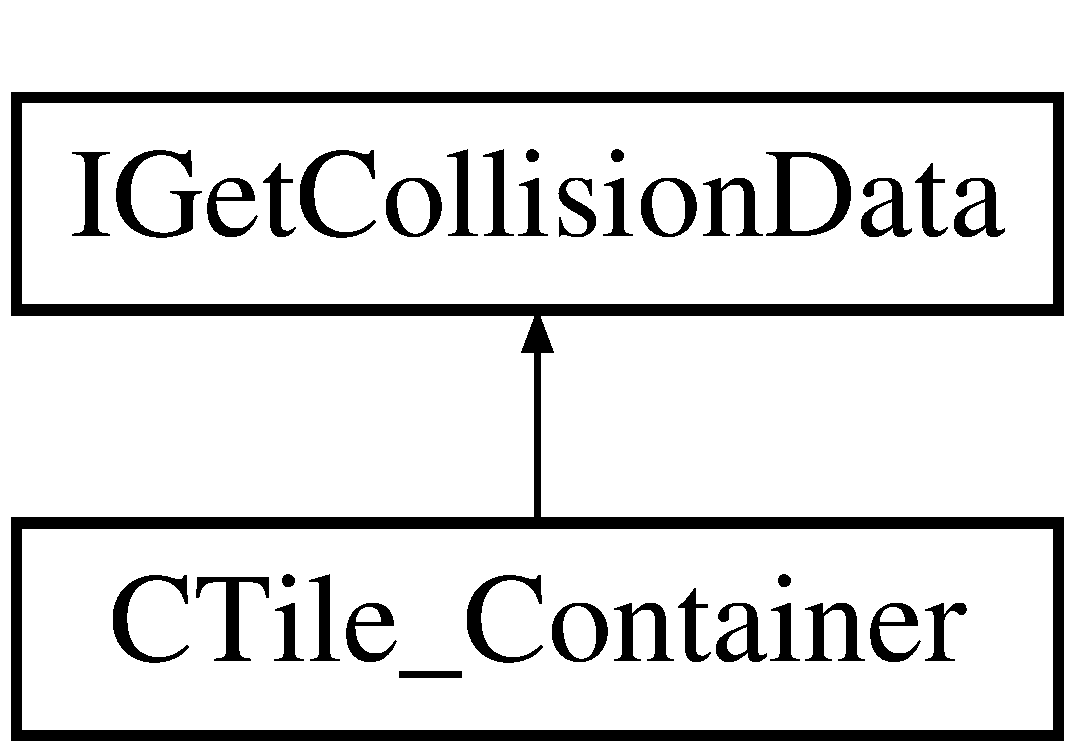
\includegraphics[height=2.000000cm]{classIGetCollisionData}
\end{center}
\end{figure}
\subsection*{Public Member Functions}
\begin{DoxyCompactItemize}
\item 
\hypertarget{classIGetCollisionData_ad31b95dda265659e5090fc2c188b30b9}{virtual void {\bfseries get\-Collisiondata} (std\-::list$<$ \hyperlink{classARenderable}{A\-Renderable} $\ast$ $>$ $\ast$p\-List)=0}\label{classIGetCollisionData_ad31b95dda265659e5090fc2c188b30b9}

\end{DoxyCompactItemize}


\subsection{Detailed Description}


Definition at line 14 of file I\-Get\-Collision\-Data.\-h.



The documentation for this class was generated from the following files\-:\begin{DoxyCompactItemize}
\item 
/home/z\-Zelman/\-Dropbox/\-Covert-\/\-Collisions Host dir/\-Covert-\/\-Collisions/src/\-Headers/I\-Get\-Collision\-Data.\-h\item 
/home/z\-Zelman/\-Dropbox/\-Covert-\/\-Collisions Host dir/\-Covert-\/\-Collisions/src/\-Interfaces/I\-Get\-Collision\-Data.\-cpp\end{DoxyCompactItemize}

\hypertarget{classIGetRenderData}{\section{I\-Get\-Render\-Data Class Reference}
\label{classIGetRenderData}\index{I\-Get\-Render\-Data@{I\-Get\-Render\-Data}}
}


A common interface for pulling relavent rendering information out of objects.  




{\ttfamily \#include $<$I\-Get\-Render\-Data.\-h$>$}



Inheritance diagram for I\-Get\-Render\-Data\-:\nopagebreak
\begin{figure}[H]
\begin{center}
\leavevmode
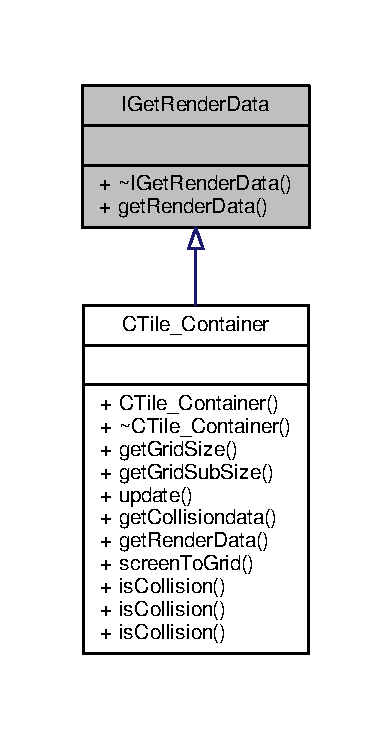
\includegraphics[width=188pt]{classIGetRenderData__inherit__graph}
\end{center}
\end{figure}


Collaboration diagram for I\-Get\-Render\-Data\-:\nopagebreak
\begin{figure}[H]
\begin{center}
\leavevmode
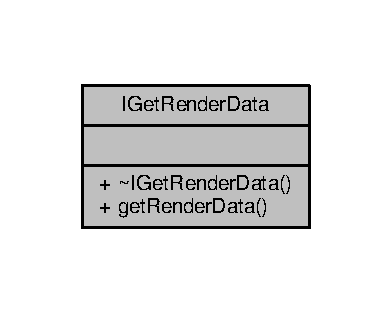
\includegraphics[width=188pt]{classIGetRenderData__coll__graph}
\end{center}
\end{figure}
\subsection*{Public Member Functions}
\begin{DoxyCompactItemize}
\item 
virtual \hyperlink{classIGetRenderData_a103a79b988144591bc820c0f28ad23c5}{$\sim$\-I\-Get\-Render\-Data} ()
\item 
virtual void \hyperlink{classIGetRenderData_ac98527f07b6d1b5030786b4848cca867}{get\-Render\-Data} (std\-::list$<$ \hyperlink{classARenderable}{A\-Renderable} $\ast$ $>$ $\ast$p\-List)=0
\begin{DoxyCompactList}\small\item\em Fills the std\-::list with objects that need to be rendered. \end{DoxyCompactList}\end{DoxyCompactItemize}


\subsection{Detailed Description}
A common interface for pulling relavent rendering information out of objects. 

Definition at line 18 of file I\-Get\-Render\-Data.\-h.



\subsection{Constructor \& Destructor Documentation}
\hypertarget{classIGetRenderData_a103a79b988144591bc820c0f28ad23c5}{\index{I\-Get\-Render\-Data@{I\-Get\-Render\-Data}!$\sim$\-I\-Get\-Render\-Data@{$\sim$\-I\-Get\-Render\-Data}}
\index{$\sim$\-I\-Get\-Render\-Data@{$\sim$\-I\-Get\-Render\-Data}!IGetRenderData@{I\-Get\-Render\-Data}}
\subsubsection[{$\sim$\-I\-Get\-Render\-Data}]{\setlength{\rightskip}{0pt plus 5cm}I\-Get\-Render\-Data\-::$\sim$\-I\-Get\-Render\-Data (
\begin{DoxyParamCaption}
{}
\end{DoxyParamCaption}
)\hspace{0.3cm}{\ttfamily [virtual]}}}\label{classIGetRenderData_a103a79b988144591bc820c0f28ad23c5}


Definition at line 5 of file I\-Get\-Render\-Data.\-cpp.



\subsection{Member Function Documentation}
\hypertarget{classIGetRenderData_ac98527f07b6d1b5030786b4848cca867}{\index{I\-Get\-Render\-Data@{I\-Get\-Render\-Data}!get\-Render\-Data@{get\-Render\-Data}}
\index{get\-Render\-Data@{get\-Render\-Data}!IGetRenderData@{I\-Get\-Render\-Data}}
\subsubsection[{get\-Render\-Data}]{\setlength{\rightskip}{0pt plus 5cm}virtual void I\-Get\-Render\-Data\-::get\-Render\-Data (
\begin{DoxyParamCaption}
\item[{std\-::list$<$ {\bf A\-Renderable} $\ast$ $>$ $\ast$}]{p\-List}
\end{DoxyParamCaption}
)\hspace{0.3cm}{\ttfamily [pure virtual]}}}\label{classIGetRenderData_ac98527f07b6d1b5030786b4848cca867}


Fills the std\-::list with objects that need to be rendered. 



Implemented in \hyperlink{classCTile__Container_a48c74611efadee522595362a79620bff}{C\-Tile\-\_\-\-Container}.



The documentation for this class was generated from the following files\-:\begin{DoxyCompactItemize}
\item 
/home/z\-Zelman/\-Dropbox/\-Covert-\/\-Collisions Host dir/\-Covert-\/\-Collisions/src/\-Headers/\hyperlink{IGetRenderData_8h}{I\-Get\-Render\-Data.\-h}\item 
/home/z\-Zelman/\-Dropbox/\-Covert-\/\-Collisions Host dir/\-Covert-\/\-Collisions/src/\-Interfaces/\hyperlink{IGetRenderData_8cpp}{I\-Get\-Render\-Data.\-cpp}\end{DoxyCompactItemize}

\hypertarget{classIUpdateable}{\section{I\-Updateable Class Reference}
\label{classIUpdateable}\index{I\-Updateable@{I\-Updateable}}
}


An interface for providing a common method to call to update the state of an object.  




{\ttfamily \#include $<$I\-Updateable.\-h$>$}



Inheritance diagram for I\-Updateable\-:
\nopagebreak
\begin{figure}[H]
\begin{center}
\leavevmode
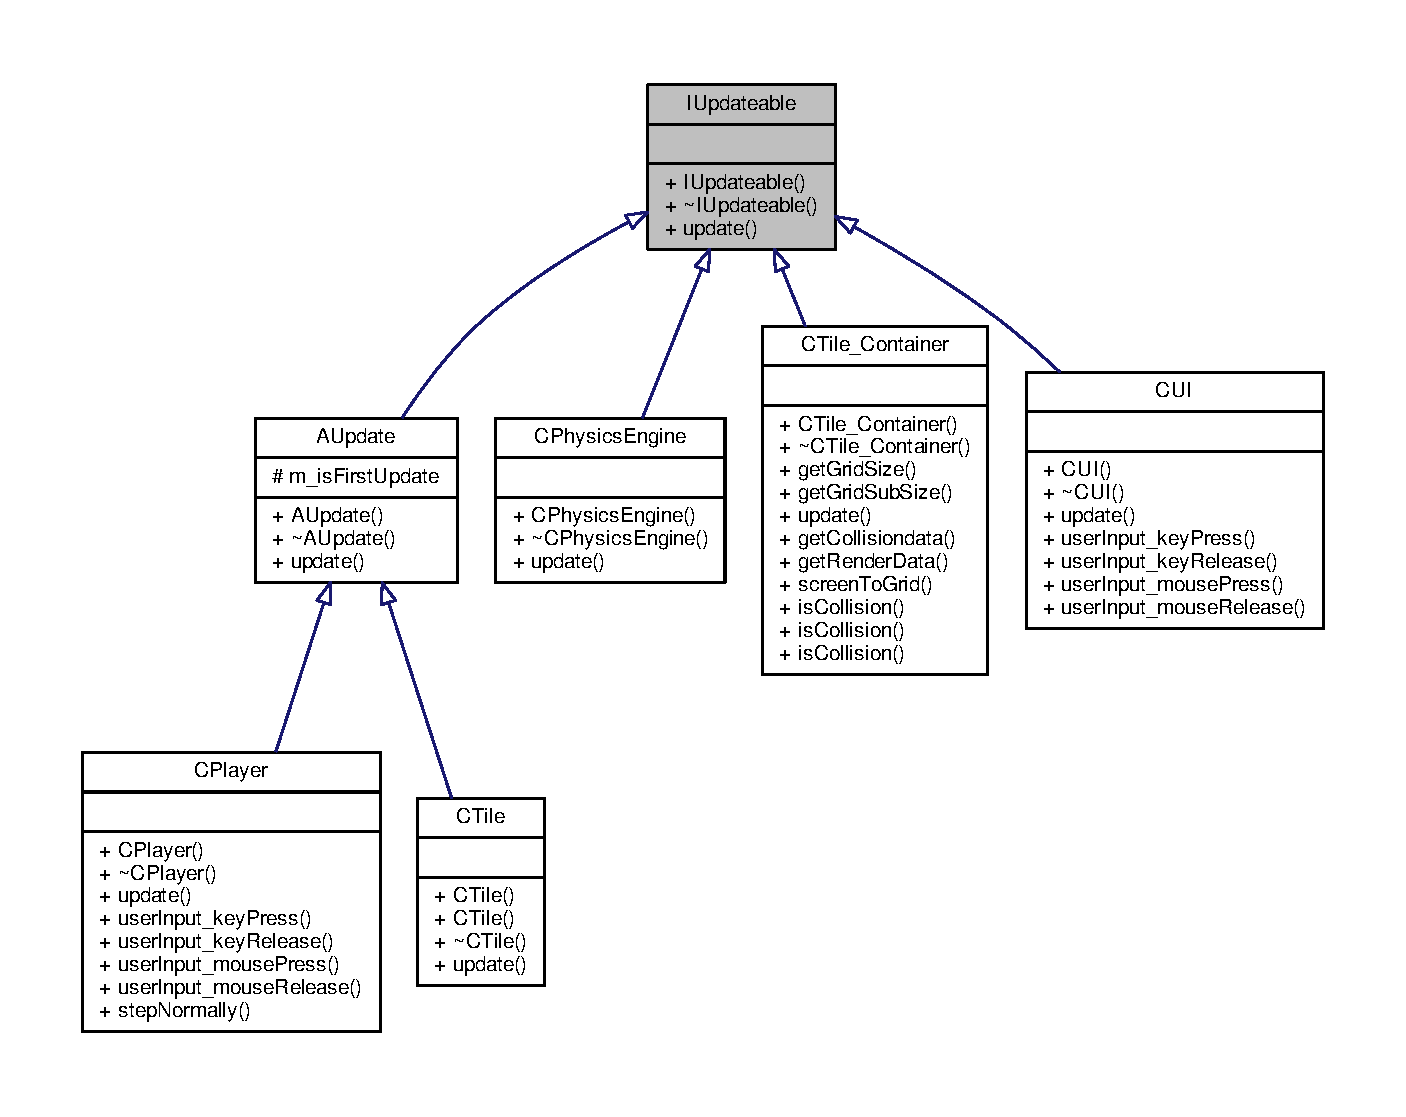
\includegraphics[width=350pt]{classIUpdateable__inherit__graph}
\end{center}
\end{figure}


Collaboration diagram for I\-Updateable\-:\nopagebreak
\begin{figure}[H]
\begin{center}
\leavevmode
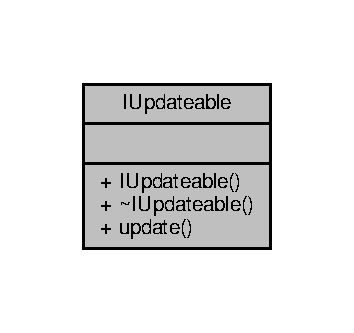
\includegraphics[width=170pt]{classIUpdateable__coll__graph}
\end{center}
\end{figure}
\subsection*{Public Member Functions}
\begin{DoxyCompactItemize}
\item 
\hyperlink{classIUpdateable_a20e6a5ae876aefb90058ad2150ac9cbc}{I\-Updateable} ()
\item 
virtual \hyperlink{classIUpdateable_a92780ea45f4696a0c546c9d7932bd5d7}{$\sim$\-I\-Updateable} ()
\item 
virtual void \hyperlink{classIUpdateable_a46d178a1ecdab33bcaad25d9b38582a5}{update} ()=0
\end{DoxyCompactItemize}


\subsection{Detailed Description}
An interface for providing a common method to call to update the state of an object. 

Definition at line 15 of file I\-Updateable.\-h.



\subsection{Constructor \& Destructor Documentation}
\hypertarget{classIUpdateable_a20e6a5ae876aefb90058ad2150ac9cbc}{\index{I\-Updateable@{I\-Updateable}!I\-Updateable@{I\-Updateable}}
\index{I\-Updateable@{I\-Updateable}!IUpdateable@{I\-Updateable}}
\subsubsection[{I\-Updateable}]{\setlength{\rightskip}{0pt plus 5cm}I\-Updateable\-::\-I\-Updateable (
\begin{DoxyParamCaption}
{}
\end{DoxyParamCaption}
)}}\label{classIUpdateable_a20e6a5ae876aefb90058ad2150ac9cbc}


Definition at line 10 of file I\-Updateable.\-cpp.

\hypertarget{classIUpdateable_a92780ea45f4696a0c546c9d7932bd5d7}{\index{I\-Updateable@{I\-Updateable}!$\sim$\-I\-Updateable@{$\sim$\-I\-Updateable}}
\index{$\sim$\-I\-Updateable@{$\sim$\-I\-Updateable}!IUpdateable@{I\-Updateable}}
\subsubsection[{$\sim$\-I\-Updateable}]{\setlength{\rightskip}{0pt plus 5cm}I\-Updateable\-::$\sim$\-I\-Updateable (
\begin{DoxyParamCaption}
{}
\end{DoxyParamCaption}
)\hspace{0.3cm}{\ttfamily [virtual]}}}\label{classIUpdateable_a92780ea45f4696a0c546c9d7932bd5d7}


Definition at line 15 of file I\-Updateable.\-cpp.



\subsection{Member Function Documentation}
\hypertarget{classIUpdateable_a46d178a1ecdab33bcaad25d9b38582a5}{\index{I\-Updateable@{I\-Updateable}!update@{update}}
\index{update@{update}!IUpdateable@{I\-Updateable}}
\subsubsection[{update}]{\setlength{\rightskip}{0pt plus 5cm}virtual void I\-Updateable\-::update (
\begin{DoxyParamCaption}
{}
\end{DoxyParamCaption}
)\hspace{0.3cm}{\ttfamily [pure virtual]}}}\label{classIUpdateable_a46d178a1ecdab33bcaad25d9b38582a5}


Implemented in \hyperlink{classCTile__Container_abe6e19de544f042671094697bb83fde9}{C\-Tile\-\_\-\-Container}, \hyperlink{classCTile_a818a17e48a7219eedac950b82c641ee0}{C\-Tile}, \hyperlink{classCPhysicsEngine_abc493897bbdb15e6787a25478730f1f5}{C\-Physics\-Engine}, \hyperlink{classCPlayer_aa77025c046956b109a76d53c12a80fa5}{C\-Player}, \hyperlink{classCUI_ab0b322040b41a6650bd625216f77b75c}{C\-U\-I}, and \hyperlink{classAUpdate_a9f5be387e467fc5eea7fc45882abd949}{A\-Update}.



The documentation for this class was generated from the following files\-:\begin{DoxyCompactItemize}
\item 
/home/z\-Zelman/\-Dropbox/\-Covert-\/\-Collisions Host dir/\-Covert-\/\-Collisions/src/\-Headers/\hyperlink{IUpdateable_8h}{I\-Updateable.\-h}\item 
/home/z\-Zelman/\-Dropbox/\-Covert-\/\-Collisions Host dir/\-Covert-\/\-Collisions/src/\-Interfaces/\hyperlink{IUpdateable_8cpp}{I\-Updateable.\-cpp}\end{DoxyCompactItemize}

\hypertarget{structAUserInput_1_1SKeyStates}{\section{A\-User\-Input\-:\-:S\-Key\-States Struct Reference}
\label{structAUserInput_1_1SKeyStates}\index{A\-User\-Input\-::\-S\-Key\-States@{A\-User\-Input\-::\-S\-Key\-States}}
}


Representation of acceptable key presses, and states of those keys.  




{\ttfamily \#include $<$A\-User\-Input.\-h$>$}

\subsection*{Public Member Functions}
\begin{DoxyCompactItemize}
\item 
\hypertarget{structAUserInput_1_1SKeyStates_a15f162c6a5b63e222fc463e0ac561798}{void {\bfseries null\-States} ()}\label{structAUserInput_1_1SKeyStates_a15f162c6a5b63e222fc463e0ac561798}

\end{DoxyCompactItemize}
\subsection*{Public Attributes}
\begin{DoxyCompactItemize}
\item 
\hypertarget{structAUserInput_1_1SKeyStates_a738215f9ee9440c8f11aa0a10fa83d42}{sf\-::\-Keyboard\-::\-Key {\bfseries up}}\label{structAUserInput_1_1SKeyStates_a738215f9ee9440c8f11aa0a10fa83d42}

\item 
\hypertarget{structAUserInput_1_1SKeyStates_a95d21217e452090bd28017c8b1110e5d}{sf\-::\-Keyboard\-::\-Key {\bfseries down}}\label{structAUserInput_1_1SKeyStates_a95d21217e452090bd28017c8b1110e5d}

\item 
\hypertarget{structAUserInput_1_1SKeyStates_aea4dc08983d8f716718a3792c779ff5c}{sf\-::\-Keyboard\-::\-Key {\bfseries left}}\label{structAUserInput_1_1SKeyStates_aea4dc08983d8f716718a3792c779ff5c}

\item 
\hypertarget{structAUserInput_1_1SKeyStates_aa9551aac4a89e8c78e20d4a12a8afcee}{sf\-::\-Keyboard\-::\-Key {\bfseries right}}\label{structAUserInput_1_1SKeyStates_aa9551aac4a89e8c78e20d4a12a8afcee}

\item 
\hypertarget{structAUserInput_1_1SKeyStates_ab227ece210dcf94947d71b21b6ea906e}{bool {\bfseries is\-Up}}\label{structAUserInput_1_1SKeyStates_ab227ece210dcf94947d71b21b6ea906e}

\item 
\hypertarget{structAUserInput_1_1SKeyStates_af06f59dc7cb752237f23e6aceac4453e}{bool {\bfseries is\-Down}}\label{structAUserInput_1_1SKeyStates_af06f59dc7cb752237f23e6aceac4453e}

\item 
\hypertarget{structAUserInput_1_1SKeyStates_afcf8a092b05f9ce67f4b2c5ea73a1f40}{bool {\bfseries is\-Right}}\label{structAUserInput_1_1SKeyStates_afcf8a092b05f9ce67f4b2c5ea73a1f40}

\item 
\hypertarget{structAUserInput_1_1SKeyStates_ab29367ed4bde7e4dd9884d75f300e5ec}{bool {\bfseries is\-Left}}\label{structAUserInput_1_1SKeyStates_ab29367ed4bde7e4dd9884d75f300e5ec}

\end{DoxyCompactItemize}


\subsection{Detailed Description}
Representation of acceptable key presses, and states of those keys. 

Definition at line 30 of file A\-User\-Input.\-h.



The documentation for this struct was generated from the following files\-:\begin{DoxyCompactItemize}
\item 
/home/z\-Zelman/\-Dropbox/\-Covert-\/\-Collisions Host dir/\-Covert-\/\-Collisions/src/\-Headers/A\-User\-Input.\-h\item 
/home/z\-Zelman/\-Dropbox/\-Covert-\/\-Collisions Host dir/\-Covert-\/\-Collisions/src/\-Abstracts/A\-User\-Input.\-cpp\end{DoxyCompactItemize}

\hypertarget{structDPhysics_1_1SPhysics}{\section{D\-Physics\-:\-:S\-Physics Struct Reference}
\label{structDPhysics_1_1SPhysics}\index{D\-Physics\-::\-S\-Physics@{D\-Physics\-::\-S\-Physics}}
}
\subsection*{Public Member Functions}
\begin{DoxyCompactItemize}
\item 
\hypertarget{structDPhysics_1_1SPhysics_aa4cf9f9d5ae6ab52b53a76d7bc507e55}{void {\bfseries null\-All} ()}\label{structDPhysics_1_1SPhysics_aa4cf9f9d5ae6ab52b53a76d7bc507e55}

\end{DoxyCompactItemize}
\subsection*{Public Attributes}
\begin{DoxyCompactItemize}
\item 
\hypertarget{structDPhysics_1_1SPhysics_aee2f0f80a53a905eb9de32d3bb12e318}{sf\-::\-Clock {\bfseries gravity\-Timer}}\label{structDPhysics_1_1SPhysics_aee2f0f80a53a905eb9de32d3bb12e318}

\item 
\hypertarget{structDPhysics_1_1SPhysics_a2654e1fd65ea35fe4119c7866fd46274}{int {\bfseries velosity\-\_\-x}}\label{structDPhysics_1_1SPhysics_a2654e1fd65ea35fe4119c7866fd46274}

\item 
\hypertarget{structDPhysics_1_1SPhysics_a58c1f8fa61d0aeece450d7ab789c5013}{int {\bfseries velosity\-\_\-y}}\label{structDPhysics_1_1SPhysics_a58c1f8fa61d0aeece450d7ab789c5013}

\item 
\hypertarget{structDPhysics_1_1SPhysics_a39163a65d84fc6d7fd0be57560cffe12}{bool {\bfseries is\-Falling}}\label{structDPhysics_1_1SPhysics_a39163a65d84fc6d7fd0be57560cffe12}

\end{DoxyCompactItemize}


\subsection{Detailed Description}


Definition at line 20 of file D\-Physics.\-h.



The documentation for this struct was generated from the following files\-:\begin{DoxyCompactItemize}
\item 
/home/z\-Zelman/\-Dropbox/\-Covert-\/\-Collisions Host dir/\-Covert-\/\-Collisions/src/\-Headers/D\-Physics.\-h\item 
/home/z\-Zelman/\-Dropbox/\-Covert-\/\-Collisions Host dir/\-Covert-\/\-Collisions/src/\-Physics/D\-Physics.\-cpp\end{DoxyCompactItemize}

\chapter{File Documentation}
\hypertarget{ARenderable_8cpp}{\section{/home/z\-Zelman/\-Dropbox/\-Covert-\/\-Collisions Host dir/\-Covert-\/\-Collisions/src/\-Abstracts/\-A\-Renderable.cpp File Reference}
\label{ARenderable_8cpp}\index{/home/z\-Zelman/\-Dropbox/\-Covert-\/\-Collisions Host dir/\-Covert-\/\-Collisions/src/\-Abstracts/\-A\-Renderable.\-cpp@{/home/z\-Zelman/\-Dropbox/\-Covert-\/\-Collisions Host dir/\-Covert-\/\-Collisions/src/\-Abstracts/\-A\-Renderable.\-cpp}}
}
{\ttfamily \#include \char`\"{}../\-Headers/\-A\-Renderable.\-h\char`\"{}}\\*
{\ttfamily \#include \char`\"{}../\-Headers/\-C\-Sprite.\-h\char`\"{}}\\*
Include dependency graph for A\-Renderable.\-cpp\-:\nopagebreak
\begin{figure}[H]
\begin{center}
\leavevmode
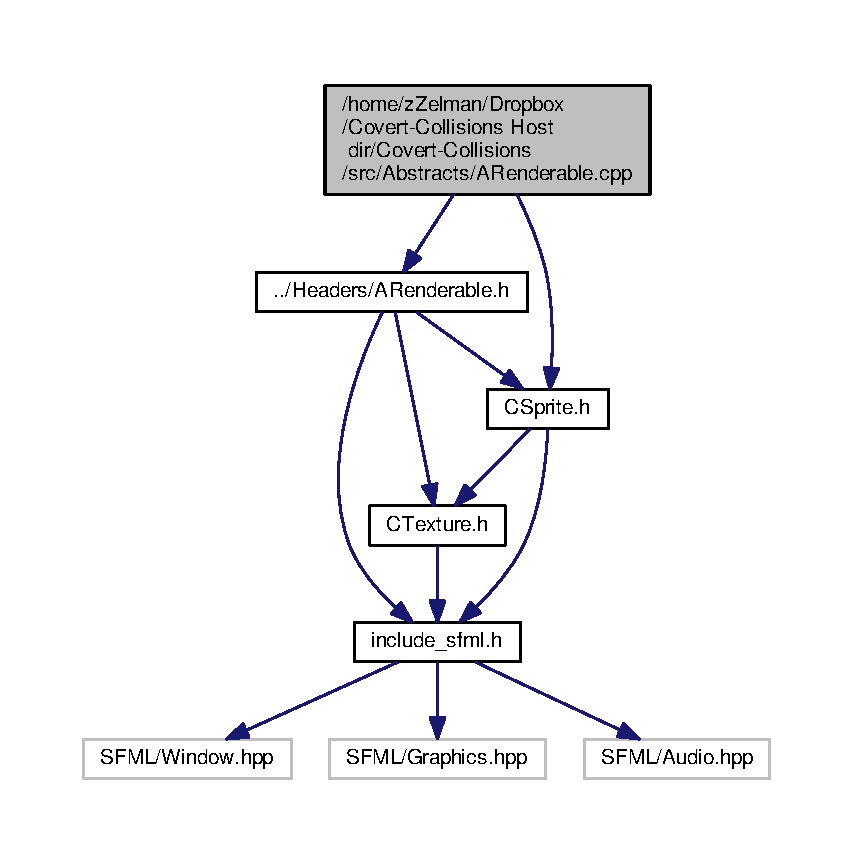
\includegraphics[width=350pt]{ARenderable_8cpp__incl}
\end{center}
\end{figure}

\hypertarget{AUpdate_8cpp}{\section{/home/z\-Zelman/\-Dropbox/\-Covert-\/\-Collisions Host dir/\-Covert-\/\-Collisions/src/\-Abstracts/\-A\-Update.cpp File Reference}
\label{AUpdate_8cpp}\index{/home/z\-Zelman/\-Dropbox/\-Covert-\/\-Collisions Host dir/\-Covert-\/\-Collisions/src/\-Abstracts/\-A\-Update.\-cpp@{/home/z\-Zelman/\-Dropbox/\-Covert-\/\-Collisions Host dir/\-Covert-\/\-Collisions/src/\-Abstracts/\-A\-Update.\-cpp}}
}
{\ttfamily \#include \char`\"{}../\-Headers/\-A\-Update.\-h\char`\"{}}\\*
Include dependency graph for A\-Update.\-cpp\-:\nopagebreak
\begin{figure}[H]
\begin{center}
\leavevmode
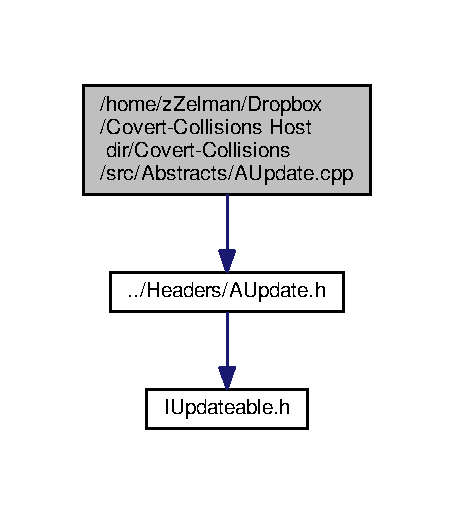
\includegraphics[width=218pt]{AUpdate_8cpp__incl}
\end{center}
\end{figure}

\hypertarget{AUserInput_8cpp}{\section{/home/z\-Zelman/\-Dropbox/\-Covert-\/\-Collisions Host dir/\-Covert-\/\-Collisions/src/\-Abstracts/\-A\-User\-Input.cpp File Reference}
\label{AUserInput_8cpp}\index{/home/z\-Zelman/\-Dropbox/\-Covert-\/\-Collisions Host dir/\-Covert-\/\-Collisions/src/\-Abstracts/\-A\-User\-Input.\-cpp@{/home/z\-Zelman/\-Dropbox/\-Covert-\/\-Collisions Host dir/\-Covert-\/\-Collisions/src/\-Abstracts/\-A\-User\-Input.\-cpp}}
}
{\ttfamily \#include \char`\"{}../\-Headers/\-A\-User\-Input.\-h\char`\"{}}\\*
Include dependency graph for A\-User\-Input.\-cpp\-:\nopagebreak
\begin{figure}[H]
\begin{center}
\leavevmode
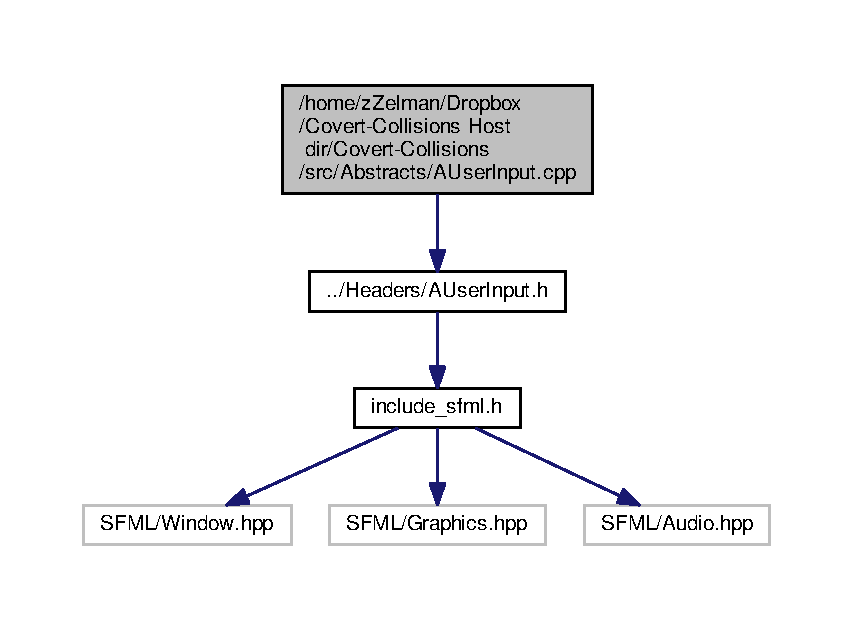
\includegraphics[width=350pt]{AUserInput_8cpp__incl}
\end{center}
\end{figure}

\hypertarget{CGame_8cpp}{\section{/home/z\-Zelman/\-Dropbox/\-Covert-\/\-Collisions Host dir/\-Covert-\/\-Collisions/src/\-C\-Game.cpp File Reference}
\label{CGame_8cpp}\index{/home/z\-Zelman/\-Dropbox/\-Covert-\/\-Collisions Host dir/\-Covert-\/\-Collisions/src/\-C\-Game.\-cpp@{/home/z\-Zelman/\-Dropbox/\-Covert-\/\-Collisions Host dir/\-Covert-\/\-Collisions/src/\-C\-Game.\-cpp}}
}
{\ttfamily \#include \char`\"{}C\-Game.\-h\char`\"{}}\\*
{\ttfamily \#include \char`\"{}Headers/include\-\_\-sfml.\-h\char`\"{}}\\*
{\ttfamily \#include $<$iostream$>$}\\*
{\ttfamily \#include $<$assert.\-h$>$}\\*
Include dependency graph for C\-Game.\-cpp\-:\nopagebreak
\begin{figure}[H]
\begin{center}
\leavevmode
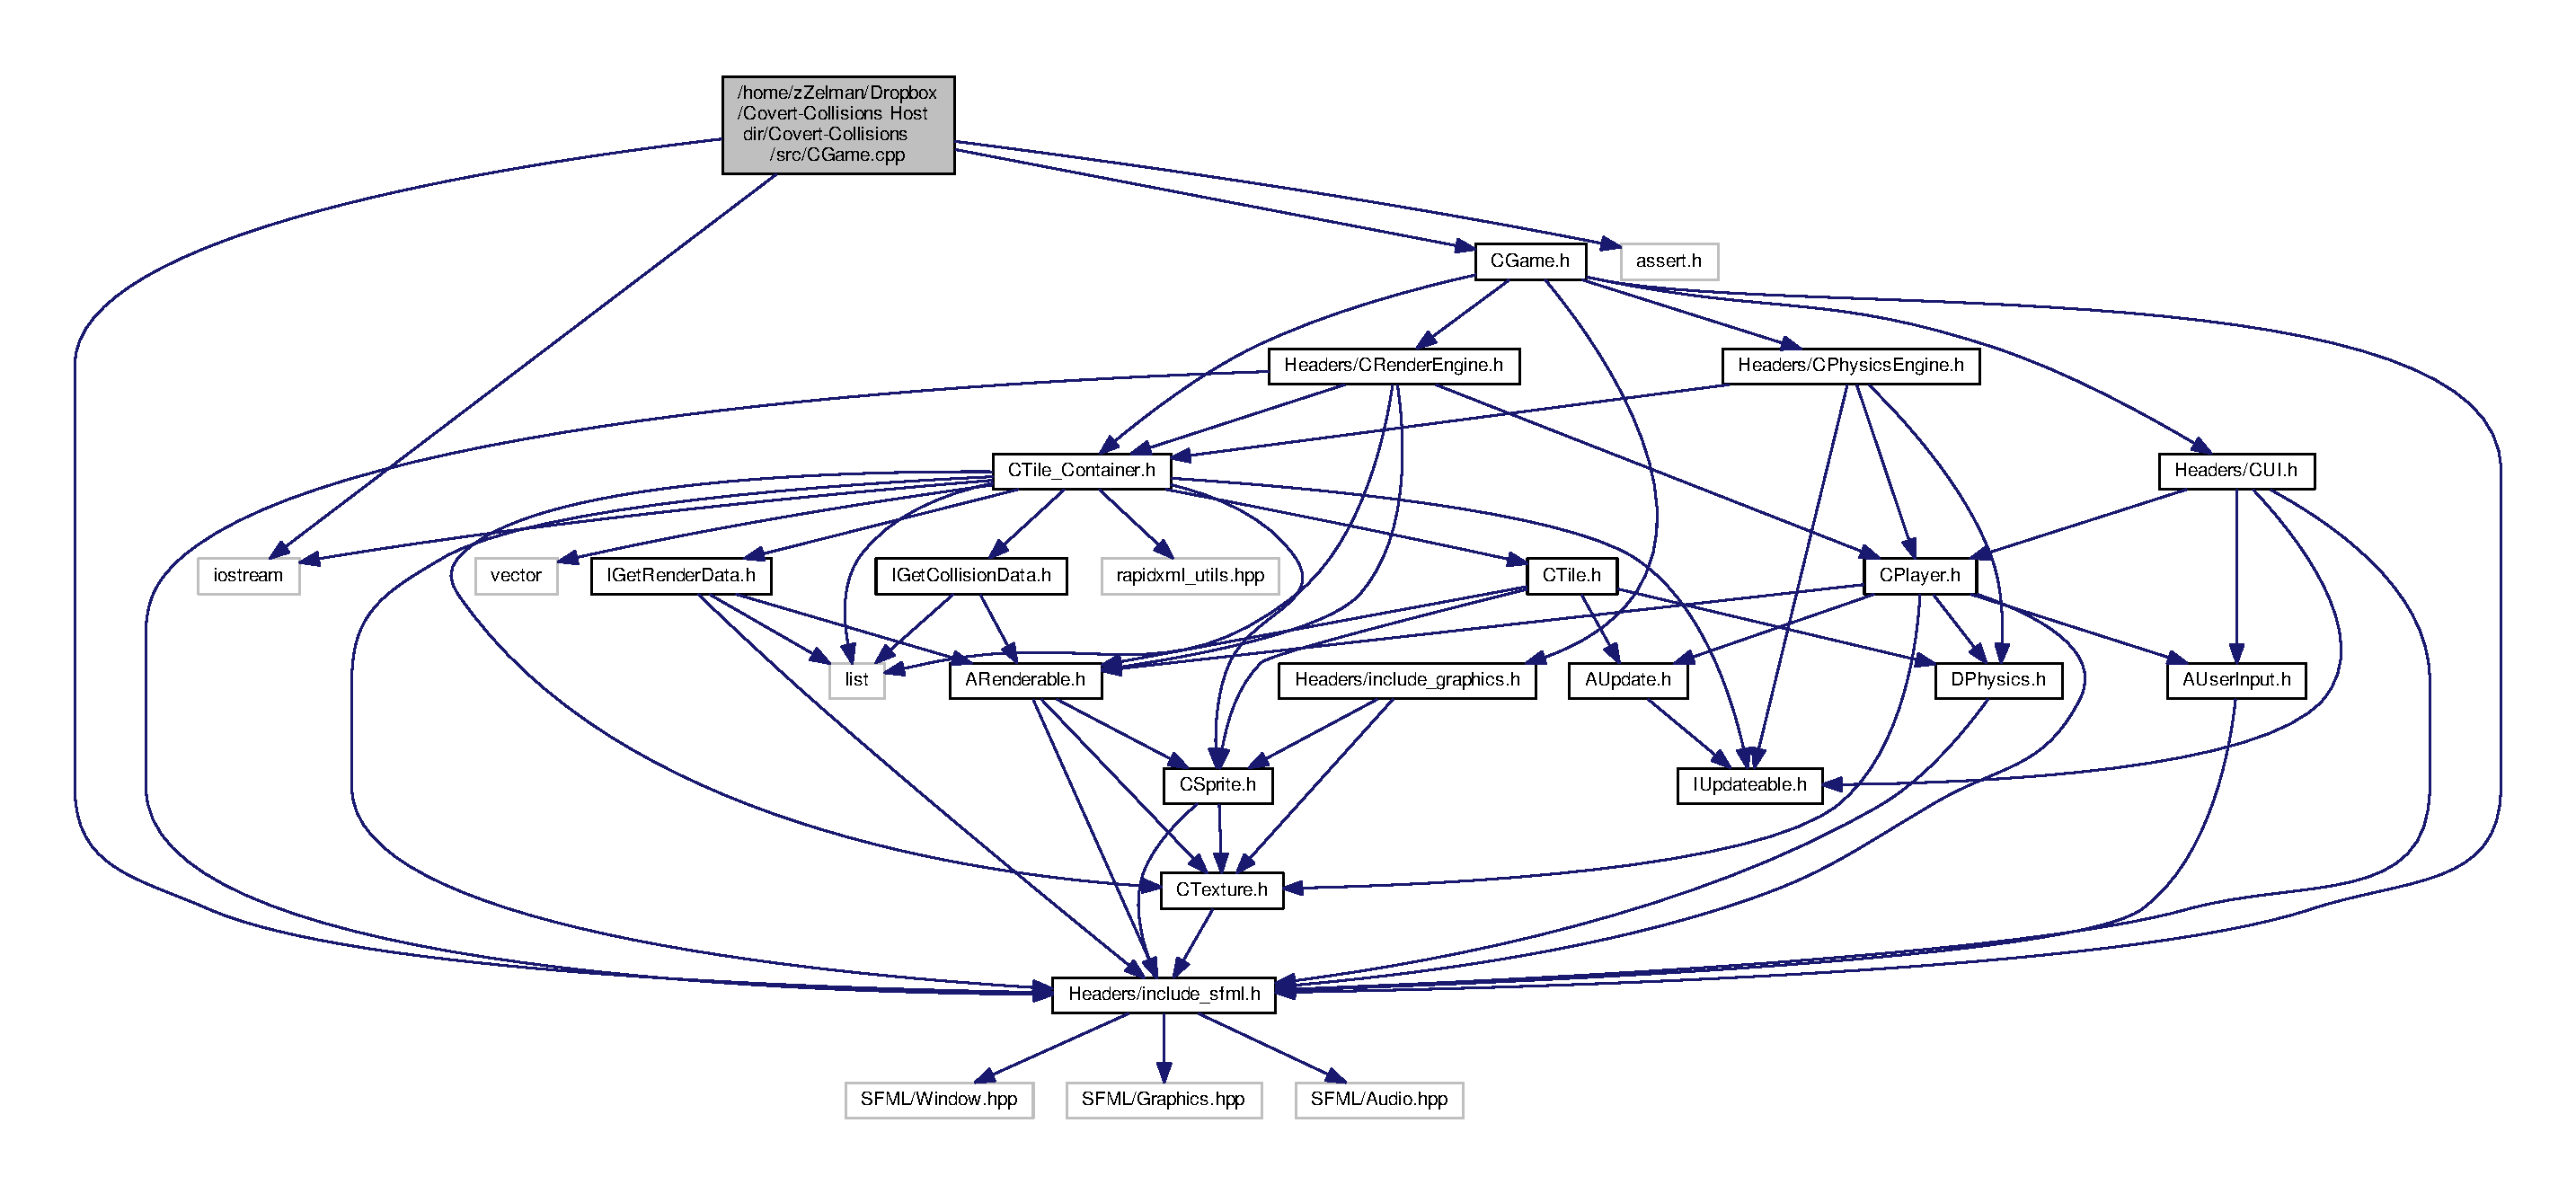
\includegraphics[width=350pt]{CGame_8cpp__incl}
\end{center}
\end{figure}

\hypertarget{CGame_8h}{\section{/home/z\-Zelman/\-Dropbox/\-Covert-\/\-Collisions Host dir/\-Covert-\/\-Collisions/src/\-C\-Game.h File Reference}
\label{CGame_8h}\index{/home/z\-Zelman/\-Dropbox/\-Covert-\/\-Collisions Host dir/\-Covert-\/\-Collisions/src/\-C\-Game.\-h@{/home/z\-Zelman/\-Dropbox/\-Covert-\/\-Collisions Host dir/\-Covert-\/\-Collisions/src/\-C\-Game.\-h}}
}
{\ttfamily \#include \char`\"{}Headers/include\-\_\-sfml.\-h\char`\"{}}\\*
{\ttfamily \#include \char`\"{}Headers/\-C\-Render\-Engine.\-h\char`\"{}}\\*
{\ttfamily \#include \char`\"{}Headers/include\-\_\-graphics.\-h\char`\"{}}\\*
{\ttfamily \#include \char`\"{}Headers/\-C\-U\-I.\-h\char`\"{}}\\*
{\ttfamily \#include \char`\"{}Headers/\-C\-Tile\-\_\-\-Container.\-h\char`\"{}}\\*
{\ttfamily \#include \char`\"{}Headers/\-C\-Physics\-Engine.\-h\char`\"{}}\\*
Include dependency graph for C\-Game.\-h\-:\nopagebreak
\begin{figure}[H]
\begin{center}
\leavevmode
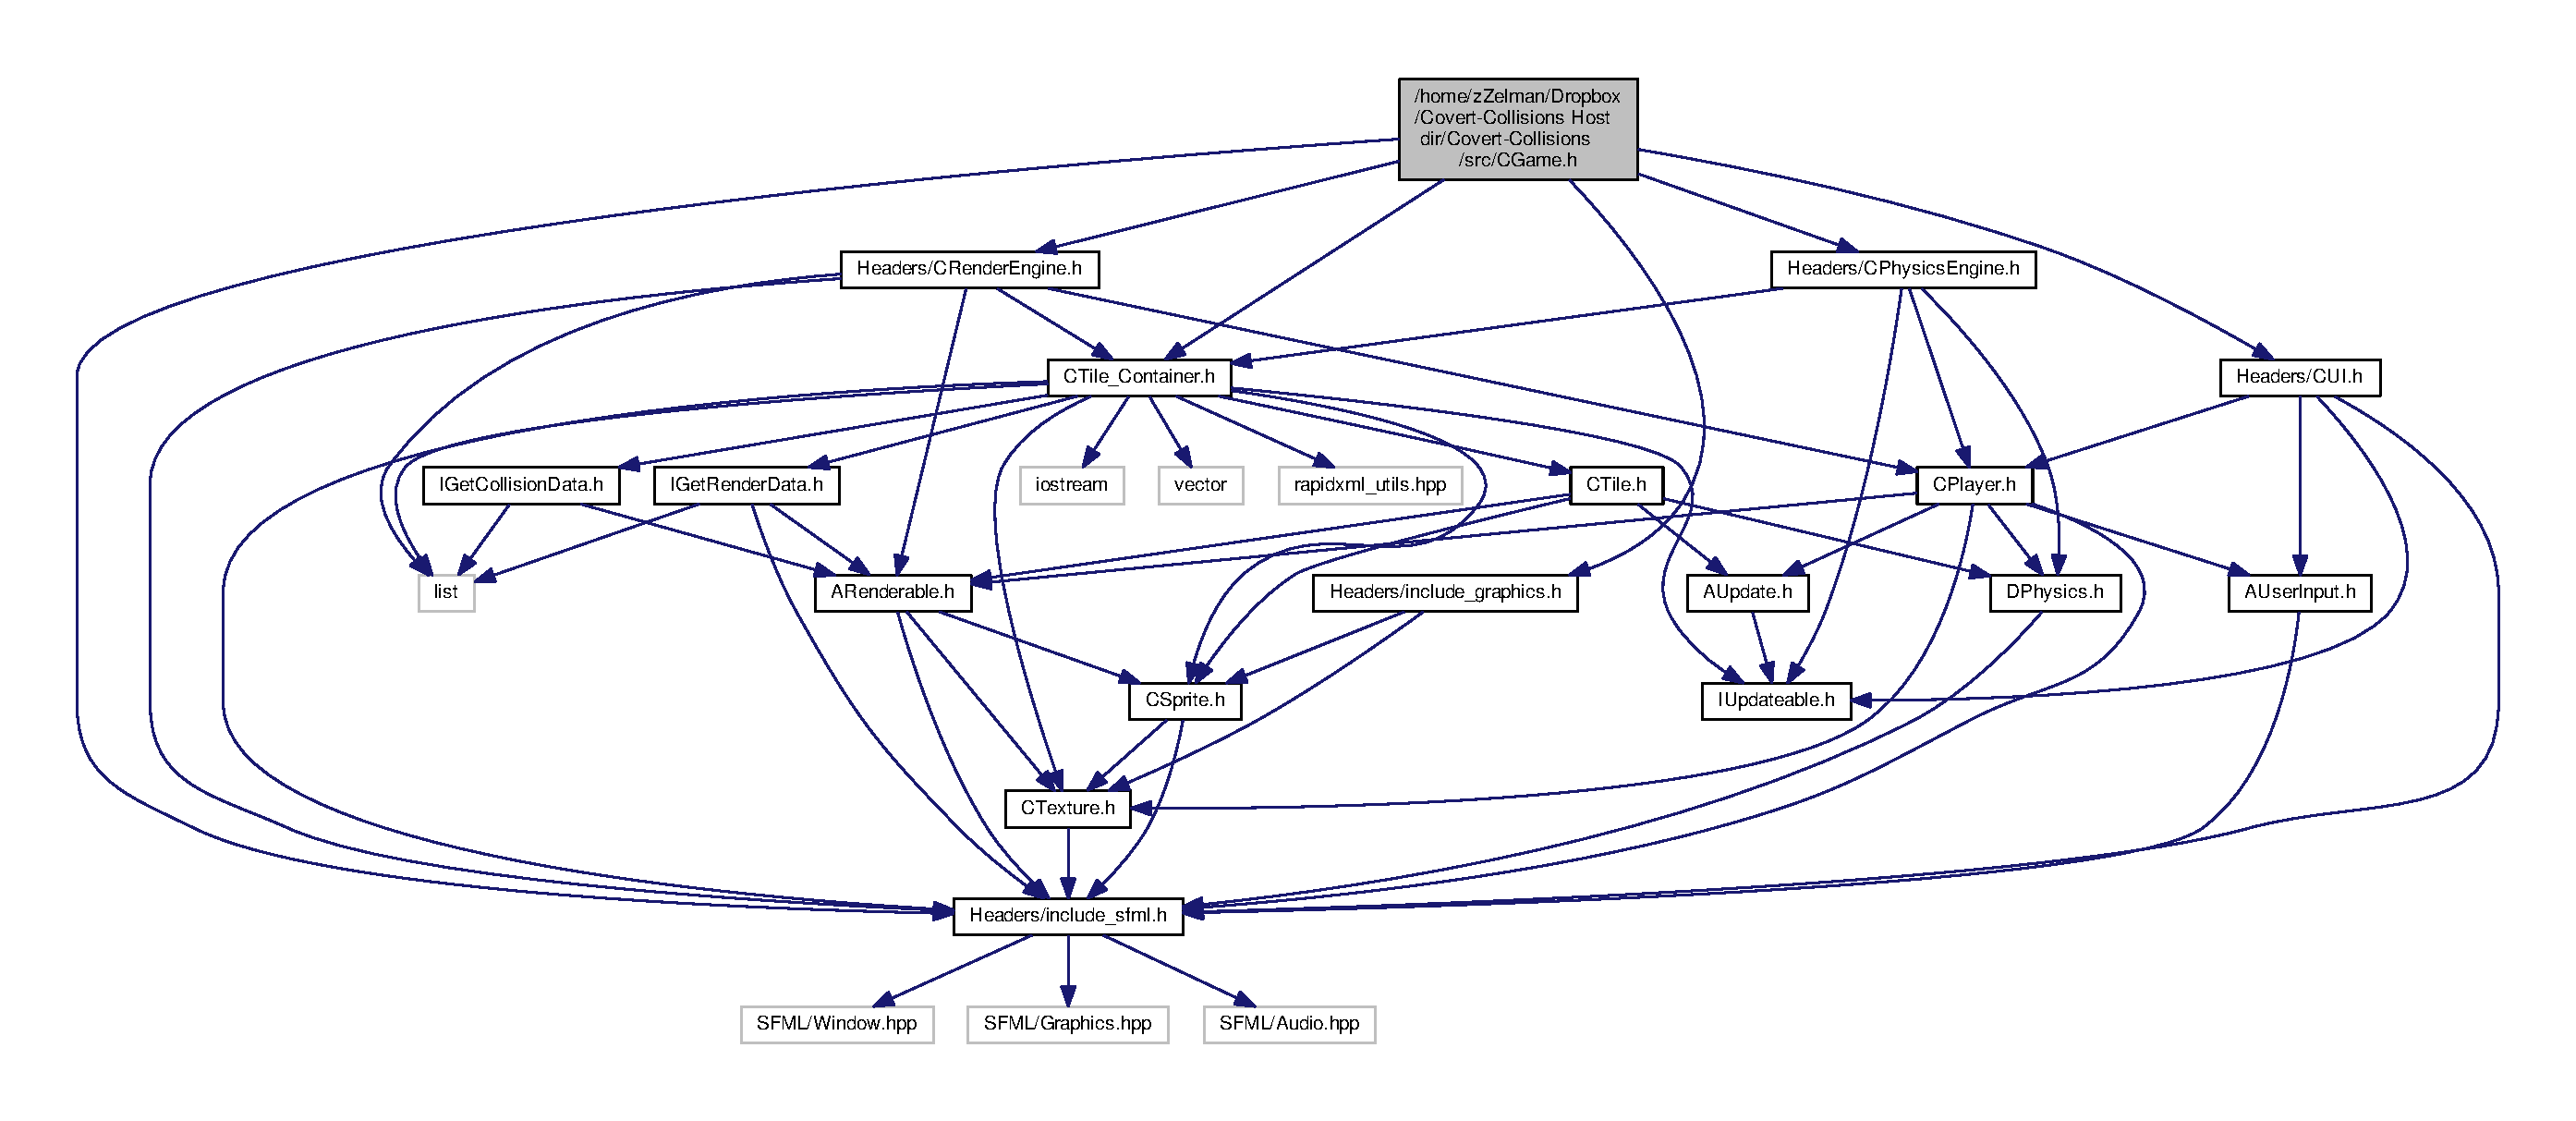
\includegraphics[width=350pt]{CGame_8h__incl}
\end{center}
\end{figure}
This graph shows which files directly or indirectly include this file\-:\nopagebreak
\begin{figure}[H]
\begin{center}
\leavevmode
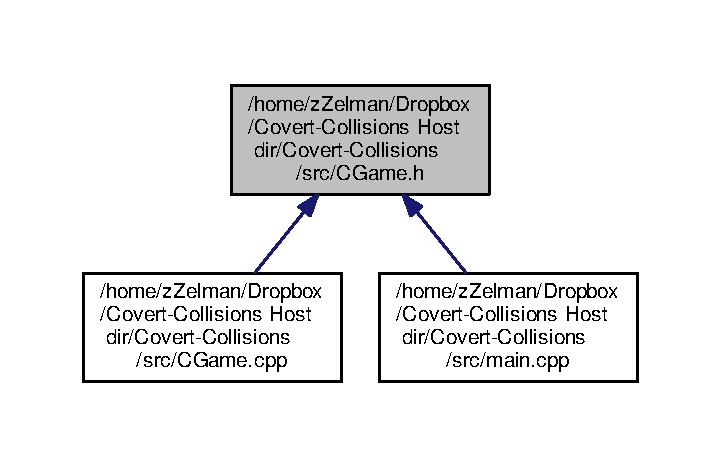
\includegraphics[width=346pt]{CGame_8h__dep__incl}
\end{center}
\end{figure}
\subsection*{Classes}
\begin{DoxyCompactItemize}
\item 
class \hyperlink{classCGame}{C\-Game}
\begin{DoxyCompactList}\small\item\em Host of game-\/loop and program flow therein, also handles S\-F\-M\-L \char`\"{}system\char`\"{} events. \end{DoxyCompactList}\end{DoxyCompactItemize}

\hypertarget{CRenderEngine_8cpp}{\section{/home/z\-Zelman/\-Dropbox/\-Covert-\/\-Collisions Host dir/\-Covert-\/\-Collisions/src/\-Graphics/\-C\-Render\-Engine.cpp File Reference}
\label{CRenderEngine_8cpp}\index{/home/z\-Zelman/\-Dropbox/\-Covert-\/\-Collisions Host dir/\-Covert-\/\-Collisions/src/\-Graphics/\-C\-Render\-Engine.\-cpp@{/home/z\-Zelman/\-Dropbox/\-Covert-\/\-Collisions Host dir/\-Covert-\/\-Collisions/src/\-Graphics/\-C\-Render\-Engine.\-cpp}}
}
{\ttfamily \#include \char`\"{}../\-Headers/\-C\-Render\-Engine.\-h\char`\"{}}\\*
{\ttfamily \#include \char`\"{}../\-Headers/include\-\_\-sfml.\-h\char`\"{}}\\*
{\ttfamily \#include $<$sstream$>$}\\*
Include dependency graph for C\-Render\-Engine.\-cpp\-:\nopagebreak
\begin{figure}[H]
\begin{center}
\leavevmode
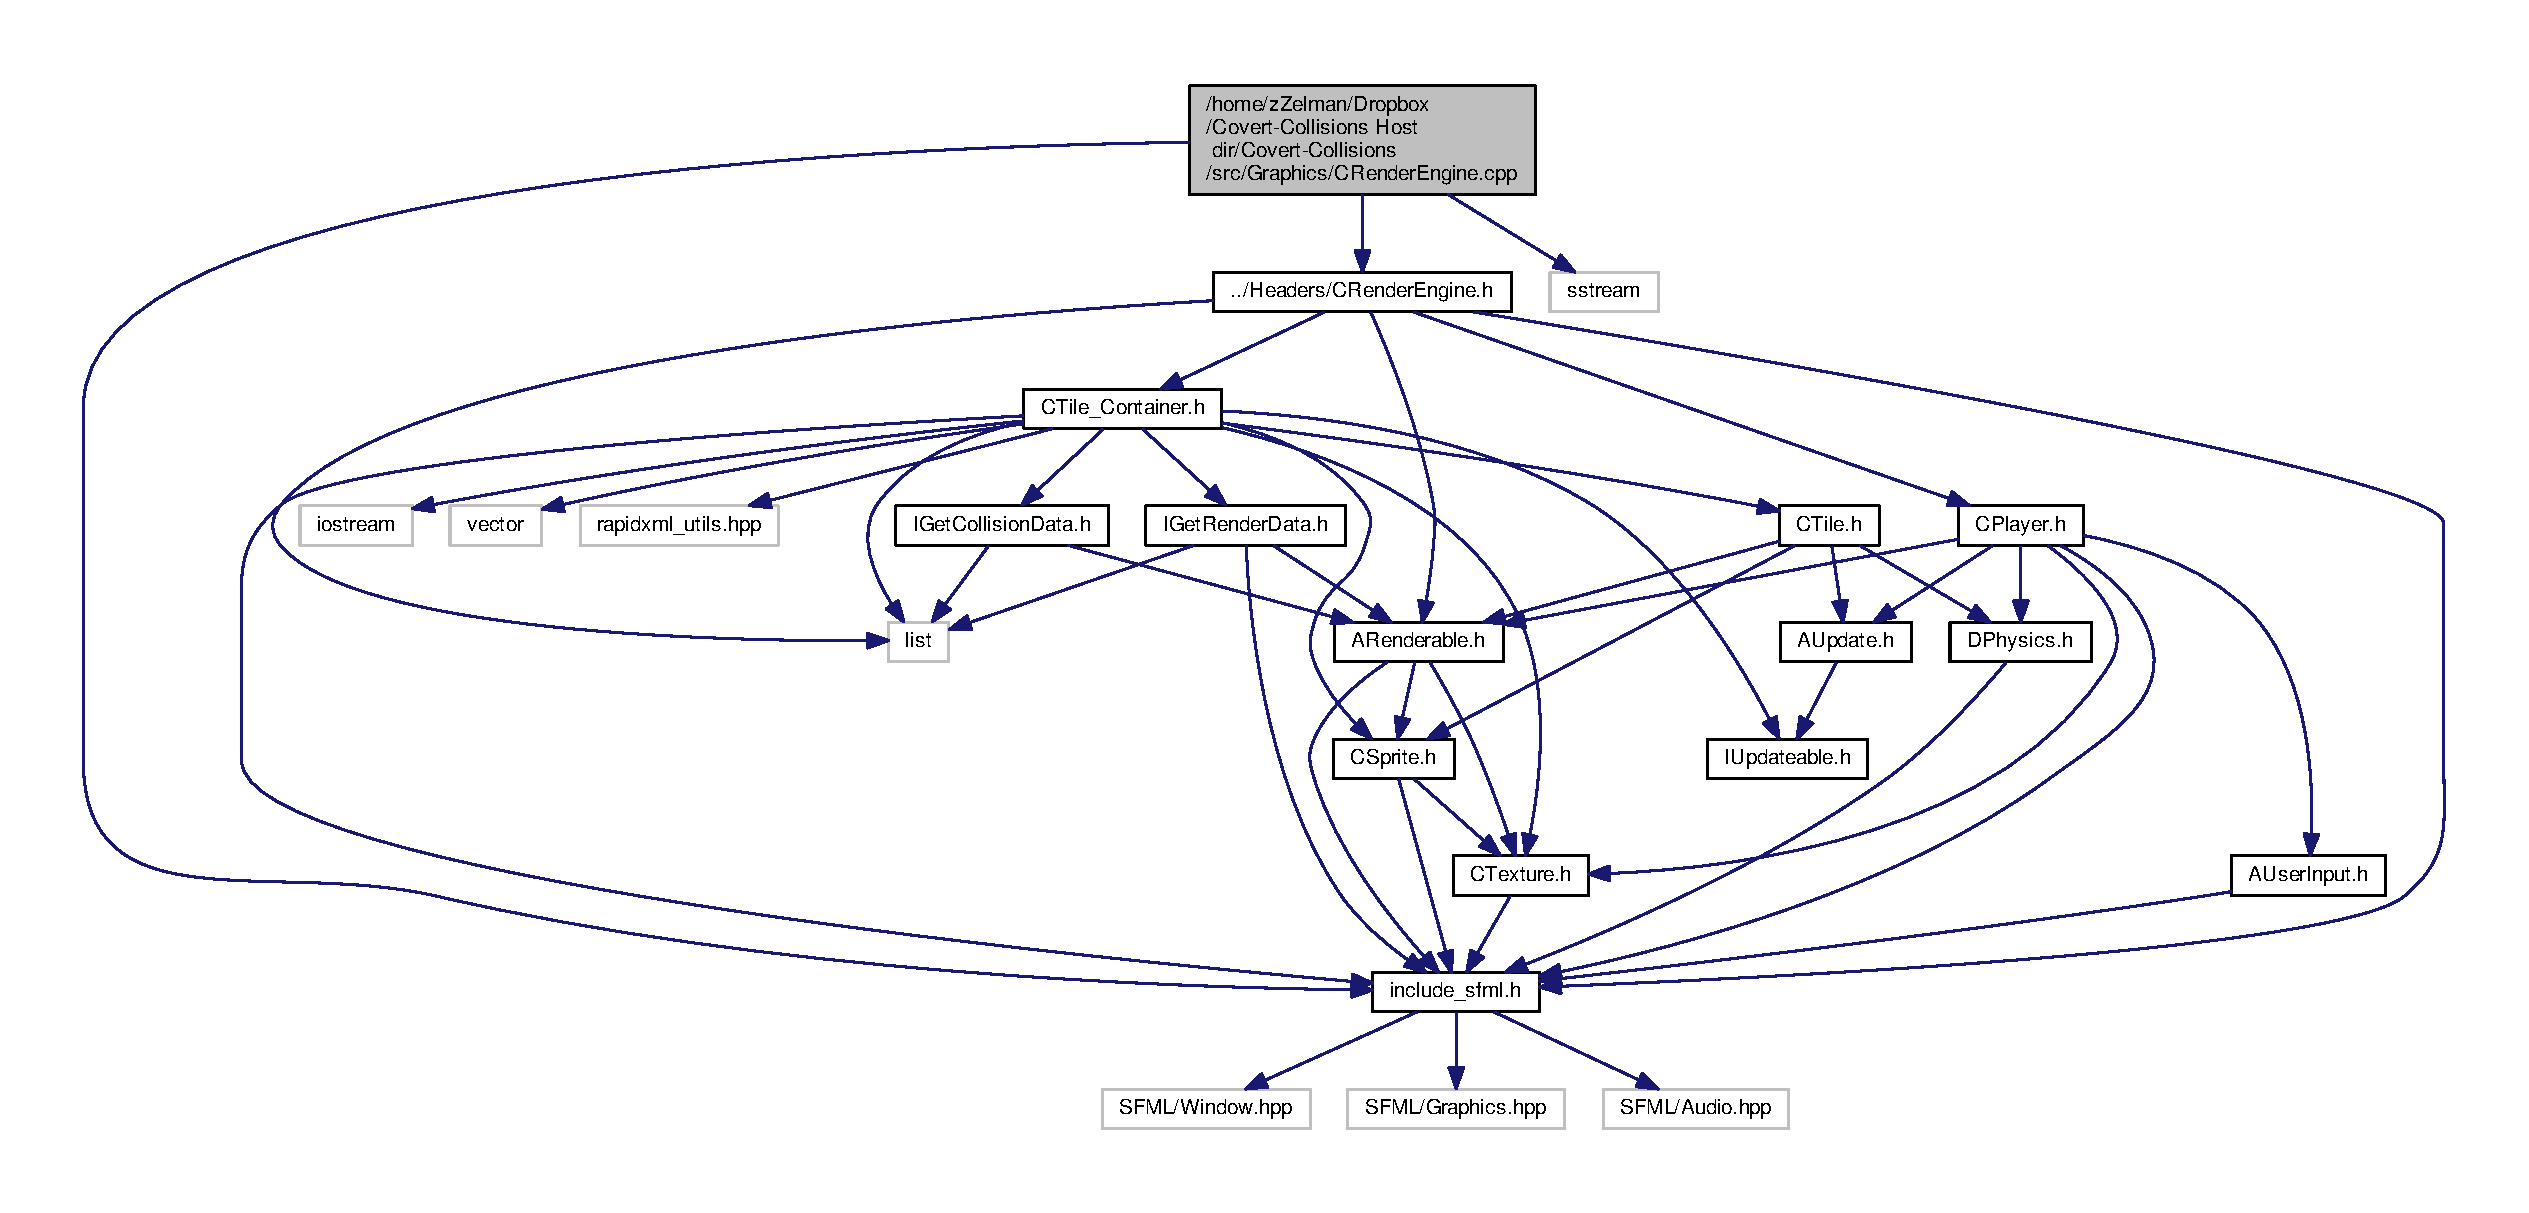
\includegraphics[width=350pt]{CRenderEngine_8cpp__incl}
\end{center}
\end{figure}

\hypertarget{CSprite_8cpp}{\section{/home/z\-Zelman/\-Dropbox/\-Covert-\/\-Collisions Host dir/\-Covert-\/\-Collisions/src/\-Graphics/\-C\-Sprite.cpp File Reference}
\label{CSprite_8cpp}\index{/home/z\-Zelman/\-Dropbox/\-Covert-\/\-Collisions Host dir/\-Covert-\/\-Collisions/src/\-Graphics/\-C\-Sprite.\-cpp@{/home/z\-Zelman/\-Dropbox/\-Covert-\/\-Collisions Host dir/\-Covert-\/\-Collisions/src/\-Graphics/\-C\-Sprite.\-cpp}}
}
{\ttfamily \#include \char`\"{}../\-Headers/\-C\-Sprite.\-h\char`\"{}}\\*
{\ttfamily \#include \char`\"{}../\-Headers/include\-\_\-sfml.\-h\char`\"{}}\\*
{\ttfamily \#include $<$assert.\-h$>$}\\*
Include dependency graph for C\-Sprite.\-cpp\-:\nopagebreak
\begin{figure}[H]
\begin{center}
\leavevmode
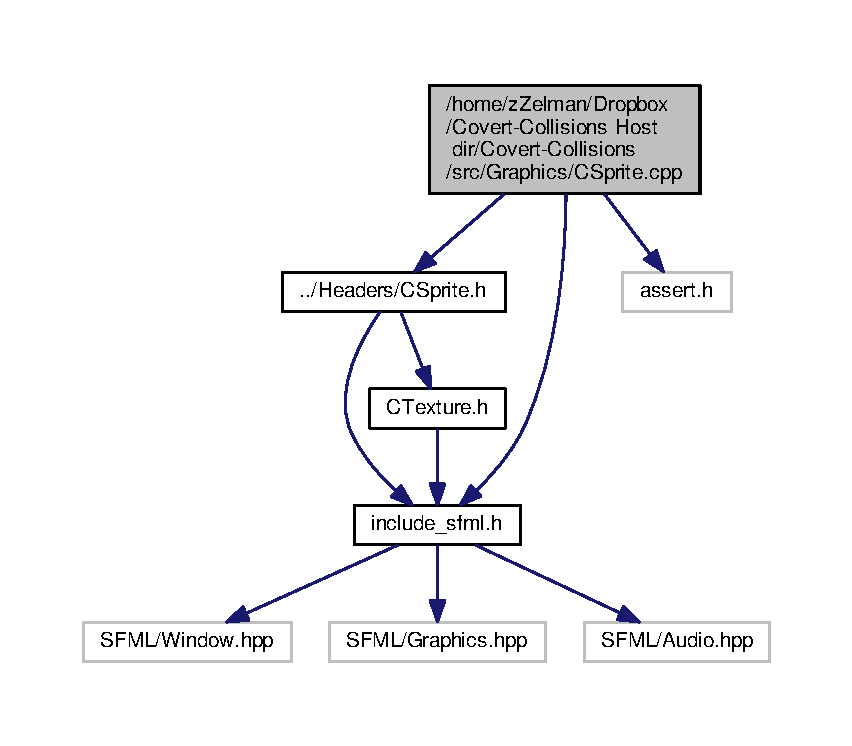
\includegraphics[width=350pt]{CSprite_8cpp__incl}
\end{center}
\end{figure}

\hypertarget{CTexture_8cpp}{\section{/home/z\-Zelman/\-Dropbox/\-Covert-\/\-Collisions Host dir/\-Covert-\/\-Collisions/src/\-Graphics/\-C\-Texture.cpp File Reference}
\label{CTexture_8cpp}\index{/home/z\-Zelman/\-Dropbox/\-Covert-\/\-Collisions Host dir/\-Covert-\/\-Collisions/src/\-Graphics/\-C\-Texture.\-cpp@{/home/z\-Zelman/\-Dropbox/\-Covert-\/\-Collisions Host dir/\-Covert-\/\-Collisions/src/\-Graphics/\-C\-Texture.\-cpp}}
}
{\ttfamily \#include \char`\"{}../\-Headers/\-C\-Texture.\-h\char`\"{}}\\*
{\ttfamily \#include \char`\"{}../\-Headers/include\-\_\-sfml.\-h\char`\"{}}\\*
{\ttfamily \#include $<$assert.\-h$>$}\\*
Include dependency graph for C\-Texture.\-cpp\-:\nopagebreak
\begin{figure}[H]
\begin{center}
\leavevmode
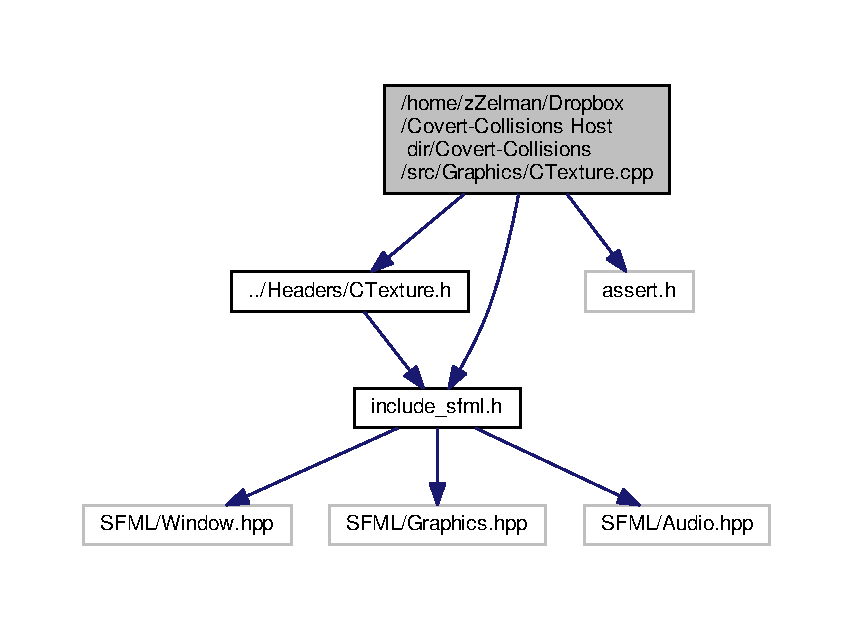
\includegraphics[width=350pt]{CTexture_8cpp__incl}
\end{center}
\end{figure}

\hypertarget{ARenderable_8h}{\section{/home/z\-Zelman/\-Dropbox/\-Covert-\/\-Collisions Host dir/\-Covert-\/\-Collisions/src/\-Headers/\-A\-Renderable.h File Reference}
\label{ARenderable_8h}\index{/home/z\-Zelman/\-Dropbox/\-Covert-\/\-Collisions Host dir/\-Covert-\/\-Collisions/src/\-Headers/\-A\-Renderable.\-h@{/home/z\-Zelman/\-Dropbox/\-Covert-\/\-Collisions Host dir/\-Covert-\/\-Collisions/src/\-Headers/\-A\-Renderable.\-h}}
}
{\ttfamily \#include \char`\"{}include\-\_\-sfml.\-h\char`\"{}}\\*
{\ttfamily \#include \char`\"{}C\-Texture.\-h\char`\"{}}\\*
{\ttfamily \#include \char`\"{}C\-Sprite.\-h\char`\"{}}\\*
Include dependency graph for A\-Renderable.\-h\-:\nopagebreak
\begin{figure}[H]
\begin{center}
\leavevmode
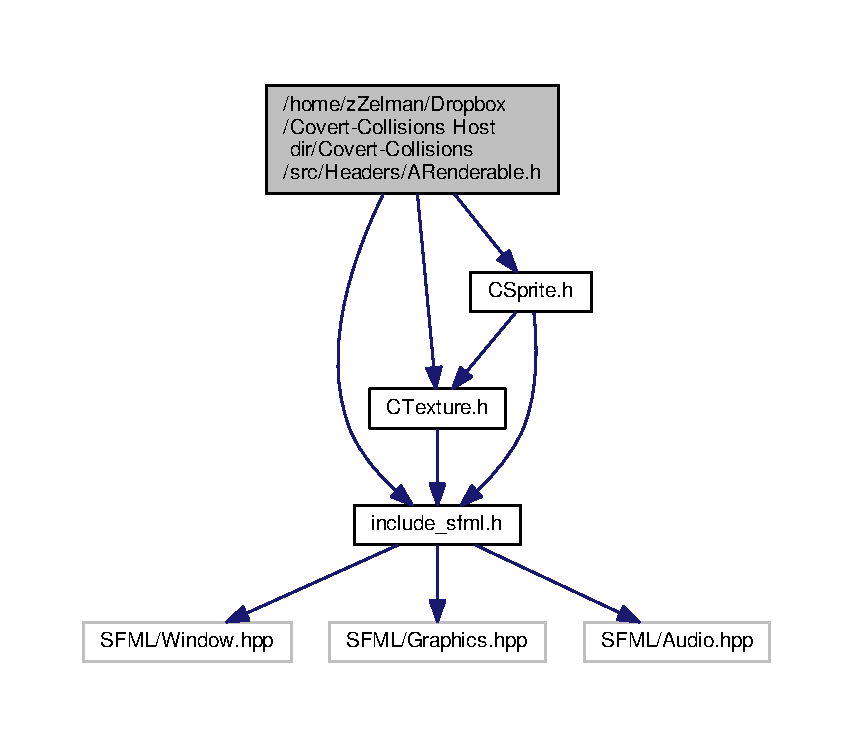
\includegraphics[width=350pt]{ARenderable_8h__incl}
\end{center}
\end{figure}
This graph shows which files directly or indirectly include this file\-:\nopagebreak
\begin{figure}[H]
\begin{center}
\leavevmode
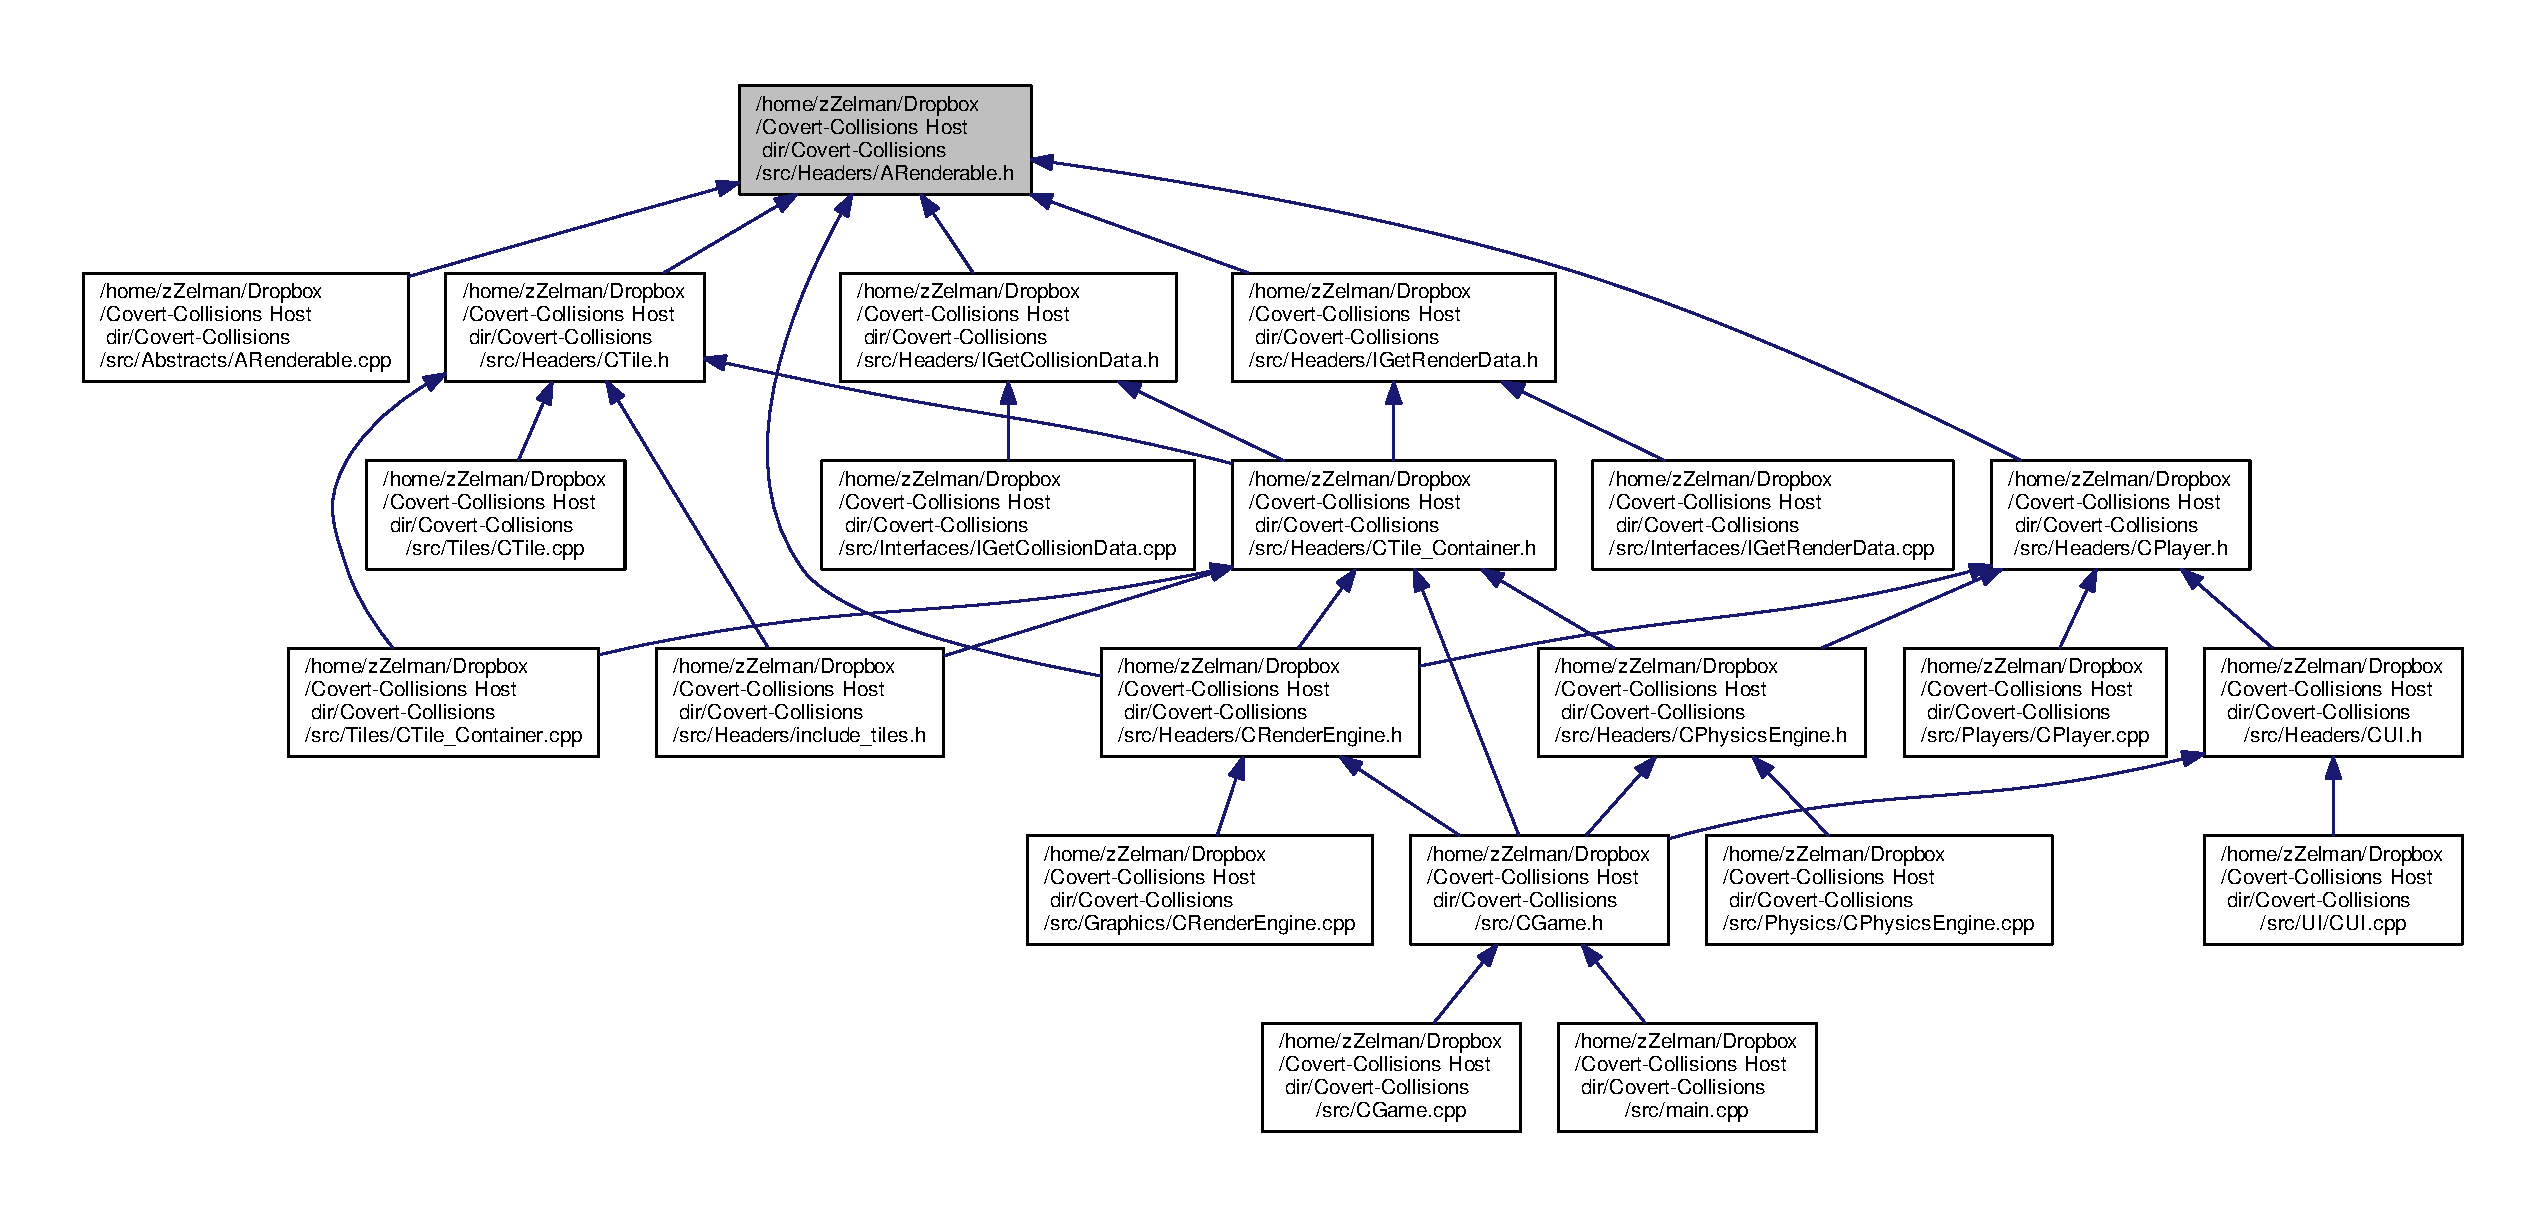
\includegraphics[width=350pt]{ARenderable_8h__dep__incl}
\end{center}
\end{figure}
\subsection*{Classes}
\begin{DoxyCompactItemize}
\item 
class \hyperlink{classARenderable}{A\-Renderable}
\begin{DoxyCompactList}\small\item\em An abstract base class for all things that can be rendered. \end{DoxyCompactList}\end{DoxyCompactItemize}

\hypertarget{AUpdate_8h}{\section{/home/z\-Zelman/\-Dropbox/\-Covert-\/\-Collisions Host dir/\-Covert-\/\-Collisions/src/\-Headers/\-A\-Update.h File Reference}
\label{AUpdate_8h}\index{/home/z\-Zelman/\-Dropbox/\-Covert-\/\-Collisions Host dir/\-Covert-\/\-Collisions/src/\-Headers/\-A\-Update.\-h@{/home/z\-Zelman/\-Dropbox/\-Covert-\/\-Collisions Host dir/\-Covert-\/\-Collisions/src/\-Headers/\-A\-Update.\-h}}
}
{\ttfamily \#include \char`\"{}I\-Updateable.\-h\char`\"{}}\\*
Include dependency graph for A\-Update.\-h\-:\nopagebreak
\begin{figure}[H]
\begin{center}
\leavevmode
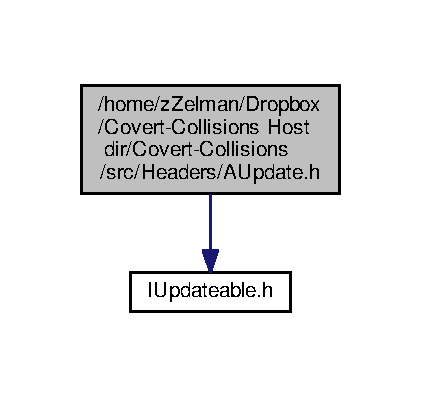
\includegraphics[width=202pt]{AUpdate_8h__incl}
\end{center}
\end{figure}
This graph shows which files directly or indirectly include this file\-:\nopagebreak
\begin{figure}[H]
\begin{center}
\leavevmode
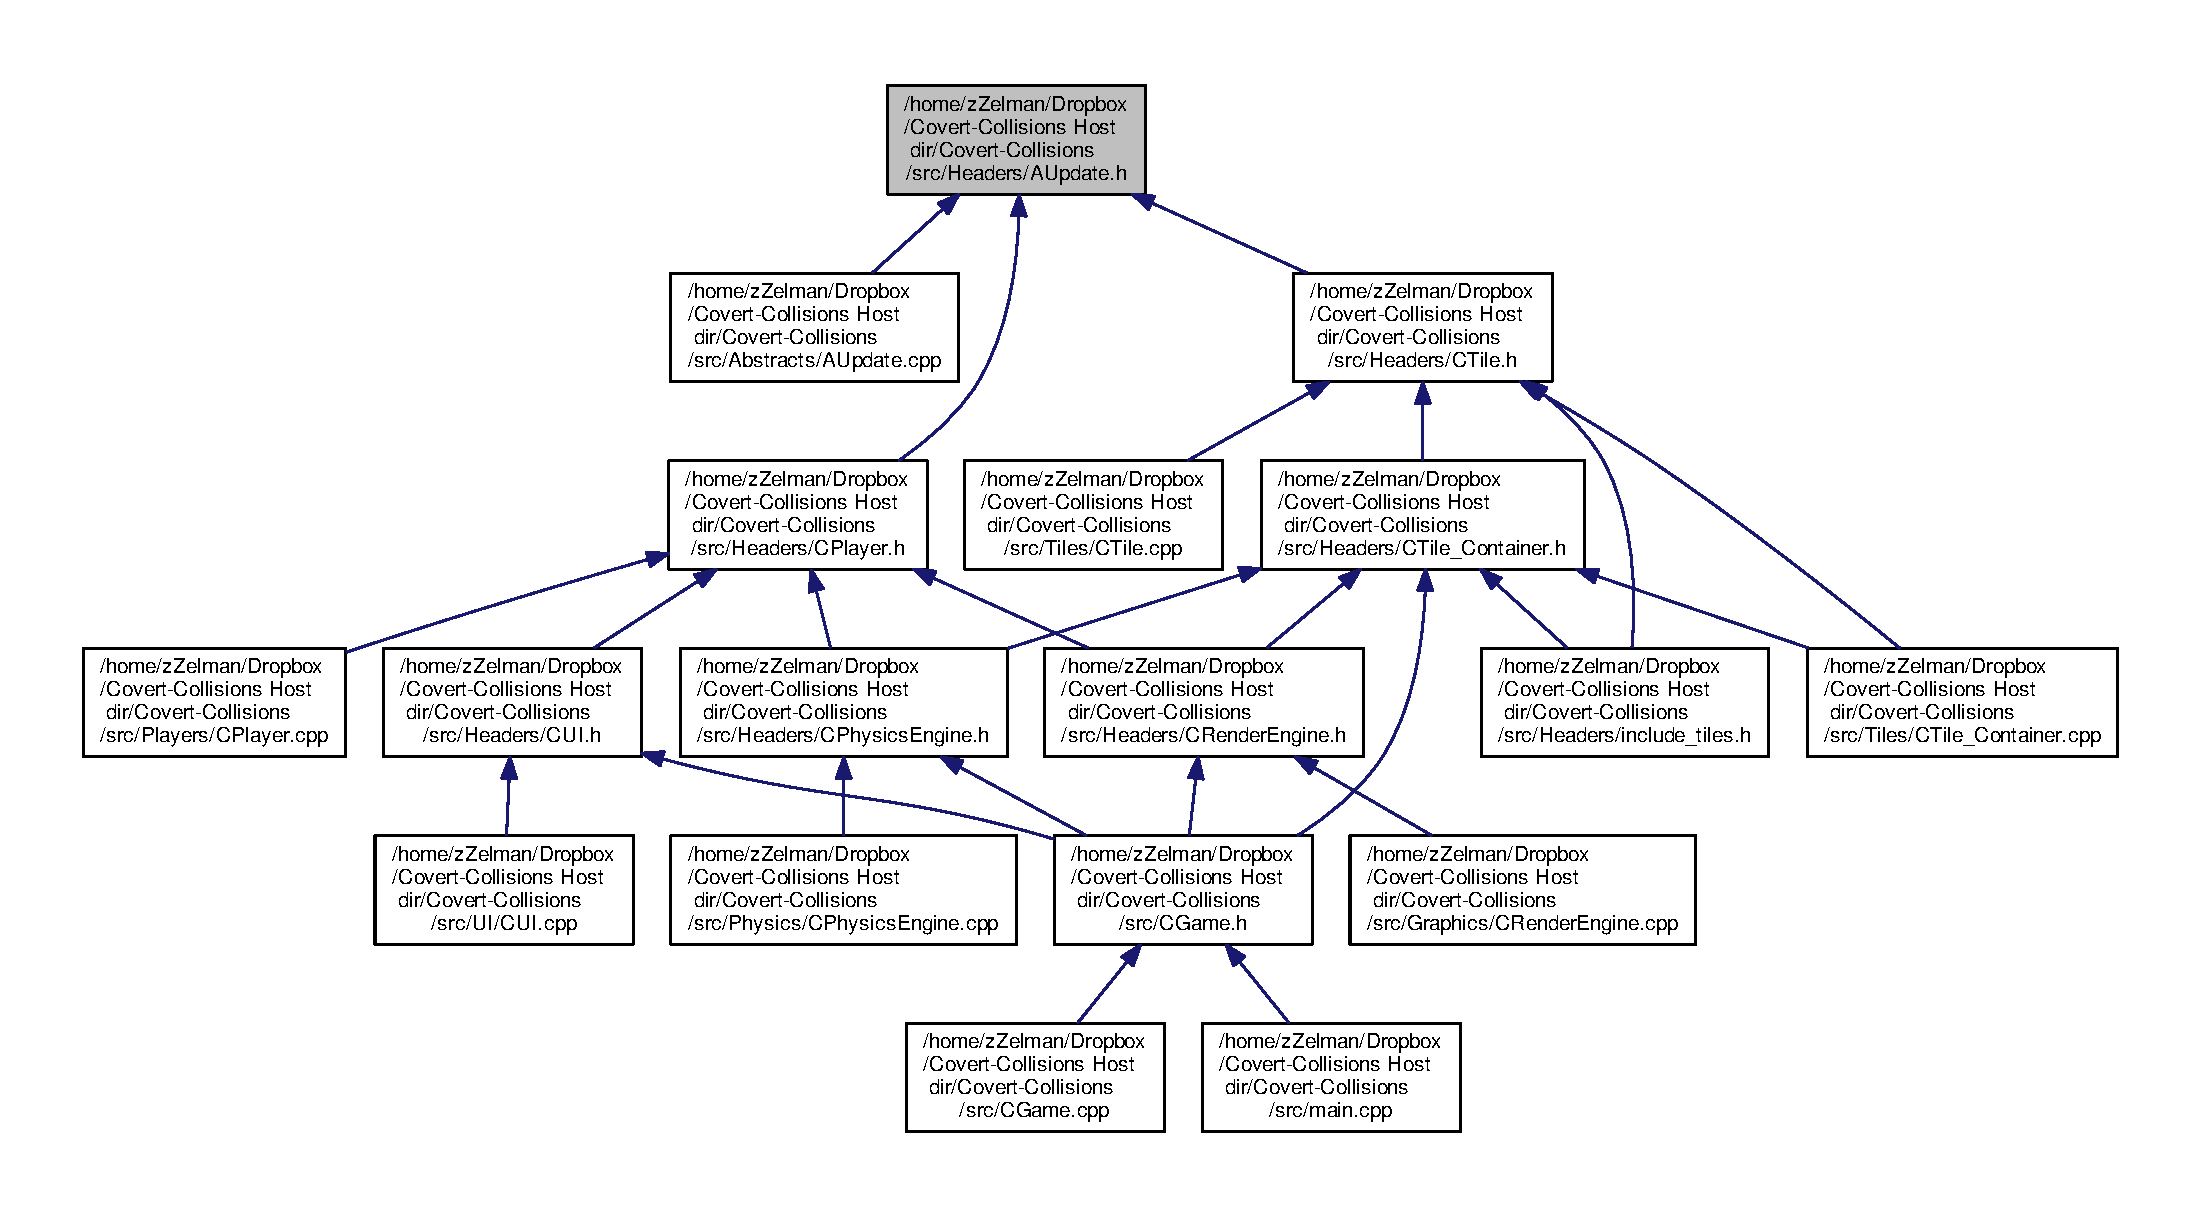
\includegraphics[width=350pt]{AUpdate_8h__dep__incl}
\end{center}
\end{figure}
\subsection*{Classes}
\begin{DoxyCompactItemize}
\item 
class \hyperlink{classAUpdate}{A\-Update}
\begin{DoxyCompactList}\small\item\em Wrapper class to I\-Updatable which only adds 1 variable. \end{DoxyCompactList}\end{DoxyCompactItemize}

\hypertarget{AUserInput_8h}{\section{/home/z\-Zelman/\-Dropbox/\-Covert-\/\-Collisions Host dir/\-Covert-\/\-Collisions/src/\-Headers/\-A\-User\-Input.h File Reference}
\label{AUserInput_8h}\index{/home/z\-Zelman/\-Dropbox/\-Covert-\/\-Collisions Host dir/\-Covert-\/\-Collisions/src/\-Headers/\-A\-User\-Input.\-h@{/home/z\-Zelman/\-Dropbox/\-Covert-\/\-Collisions Host dir/\-Covert-\/\-Collisions/src/\-Headers/\-A\-User\-Input.\-h}}
}
{\ttfamily \#include \char`\"{}include\-\_\-sfml.\-h\char`\"{}}\\*
Include dependency graph for A\-User\-Input.\-h\-:\nopagebreak
\begin{figure}[H]
\begin{center}
\leavevmode
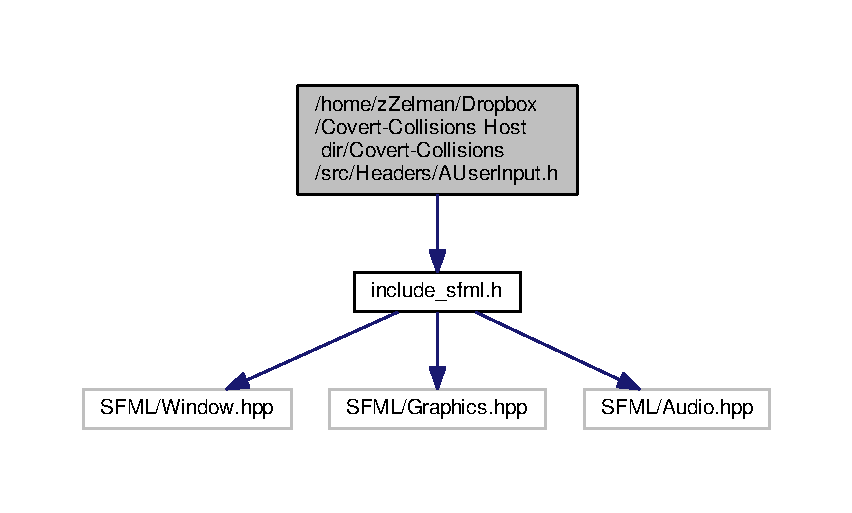
\includegraphics[width=350pt]{AUserInput_8h__incl}
\end{center}
\end{figure}
This graph shows which files directly or indirectly include this file\-:\nopagebreak
\begin{figure}[H]
\begin{center}
\leavevmode
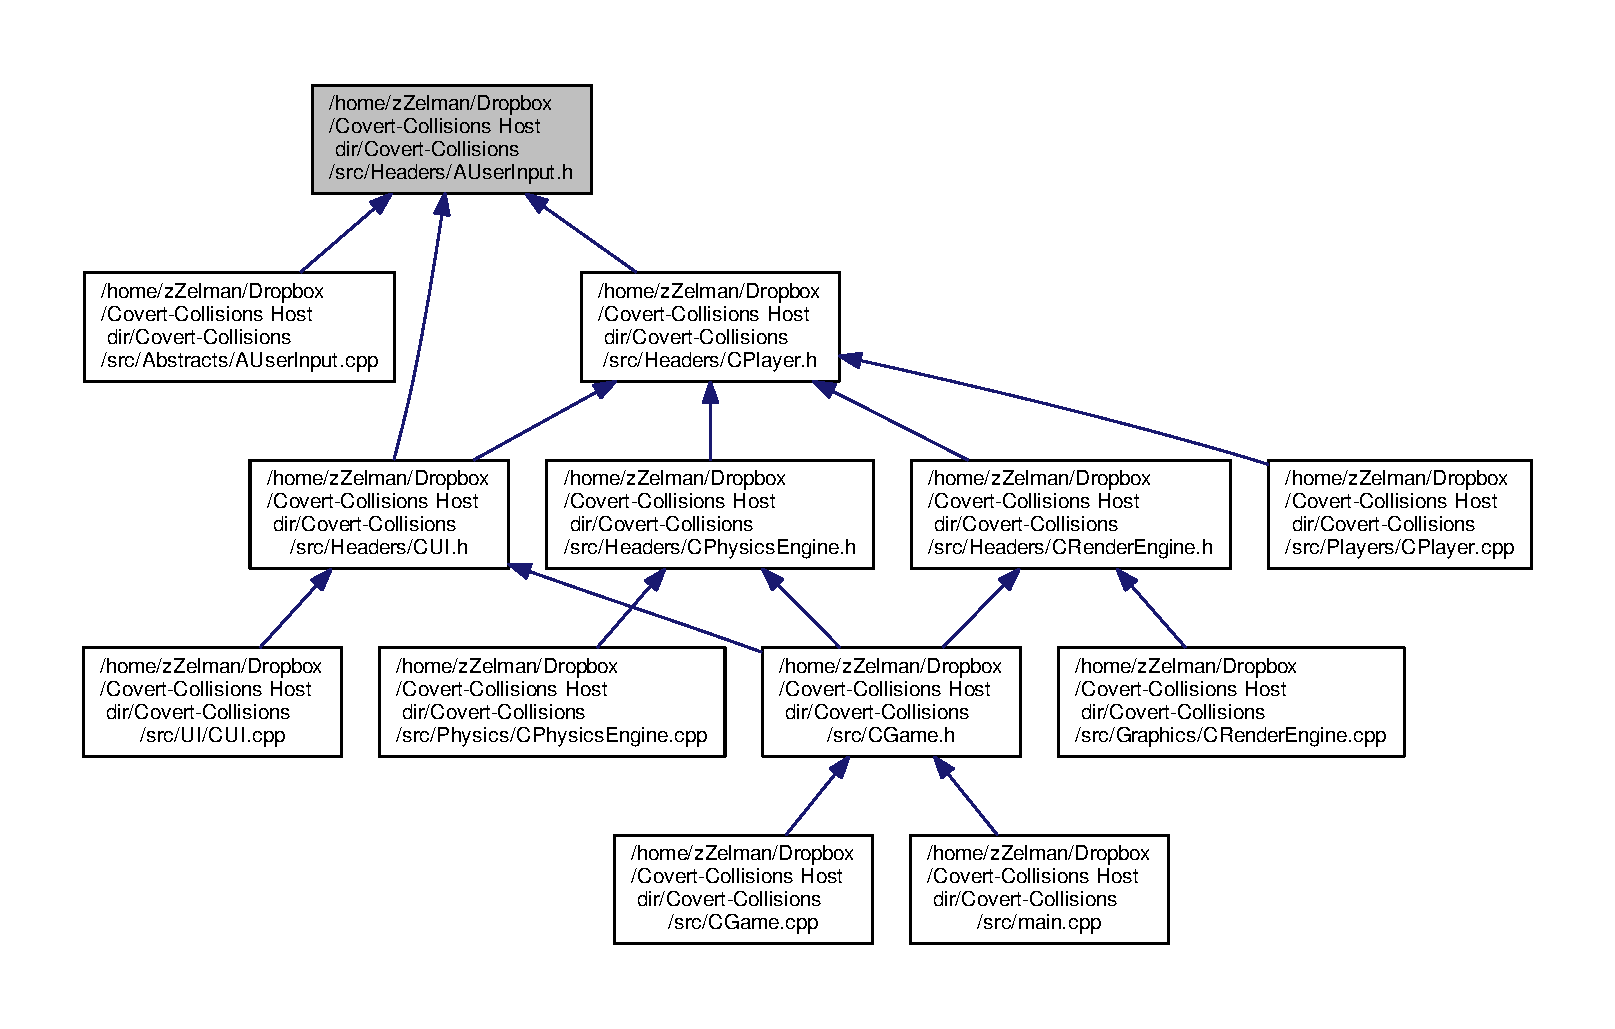
\includegraphics[width=350pt]{AUserInput_8h__dep__incl}
\end{center}
\end{figure}
\subsection*{Classes}
\begin{DoxyCompactItemize}
\item 
class \hyperlink{classAUserInput}{A\-User\-Input}
\begin{DoxyCompactList}\small\item\em Abstract class which decomposes the different types of user input. \end{DoxyCompactList}\item 
struct \hyperlink{structAUserInput_1_1SKeyStates}{A\-User\-Input\-::\-S\-Key\-States}
\begin{DoxyCompactList}\small\item\em Representation of acceptable key presses, and states of those keys. \end{DoxyCompactList}\end{DoxyCompactItemize}

\hypertarget{CPhysicsEngine_8h}{\section{/home/z\-Zelman/\-Dropbox/\-Covert-\/\-Collisions Host dir/\-Covert-\/\-Collisions/src/\-Headers/\-C\-Physics\-Engine.h File Reference}
\label{CPhysicsEngine_8h}\index{/home/z\-Zelman/\-Dropbox/\-Covert-\/\-Collisions Host dir/\-Covert-\/\-Collisions/src/\-Headers/\-C\-Physics\-Engine.\-h@{/home/z\-Zelman/\-Dropbox/\-Covert-\/\-Collisions Host dir/\-Covert-\/\-Collisions/src/\-Headers/\-C\-Physics\-Engine.\-h}}
}
{\ttfamily \#include \char`\"{}C\-Tile\-\_\-\-Container.\-h\char`\"{}}\\*
{\ttfamily \#include \char`\"{}C\-Player.\-h\char`\"{}}\\*
{\ttfamily \#include \char`\"{}I\-Updateable.\-h\char`\"{}}\\*
{\ttfamily \#include \char`\"{}D\-Physics.\-h\char`\"{}}\\*
Include dependency graph for C\-Physics\-Engine.\-h\-:\nopagebreak
\begin{figure}[H]
\begin{center}
\leavevmode
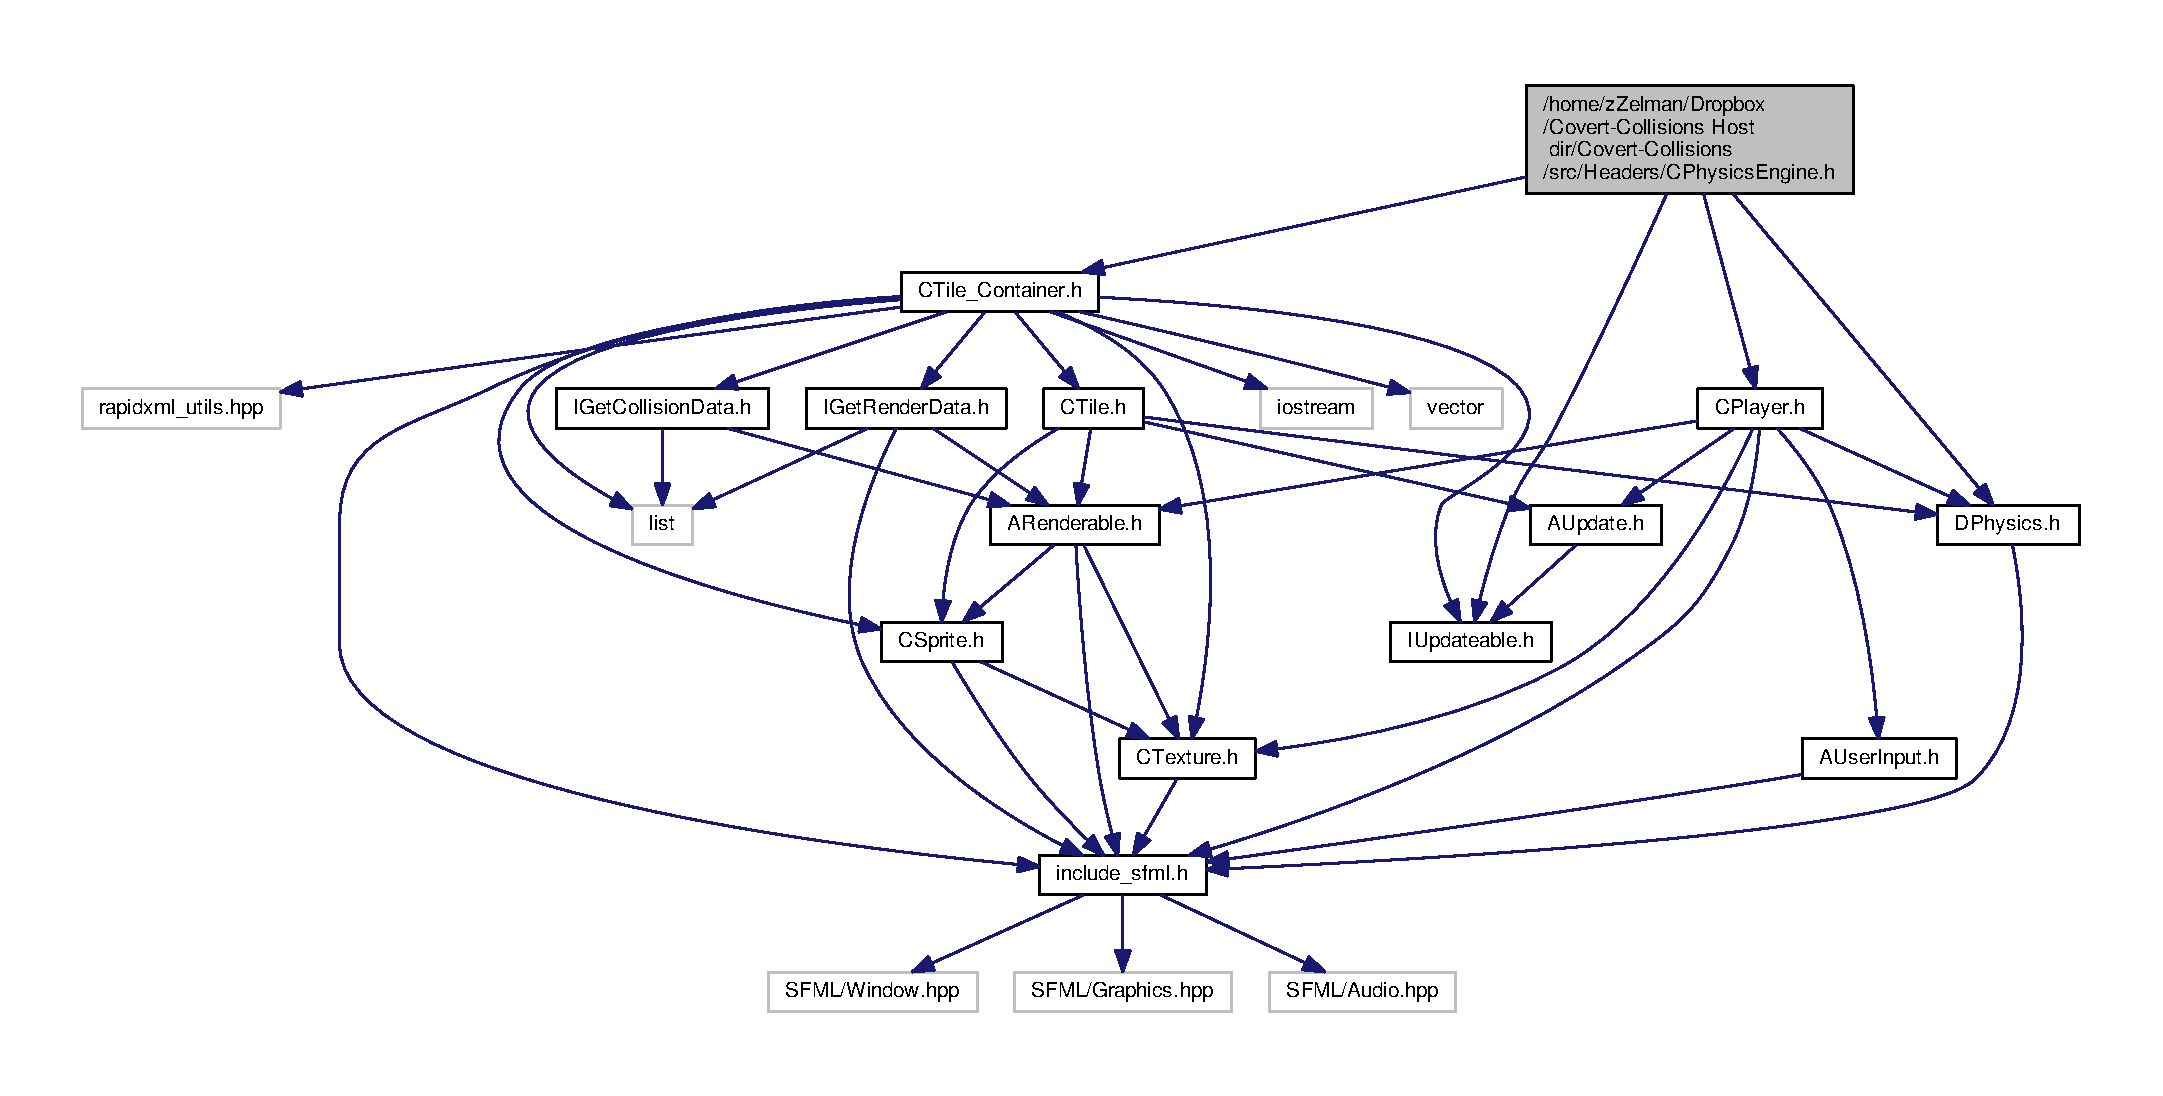
\includegraphics[width=350pt]{CPhysicsEngine_8h__incl}
\end{center}
\end{figure}
This graph shows which files directly or indirectly include this file\-:\nopagebreak
\begin{figure}[H]
\begin{center}
\leavevmode
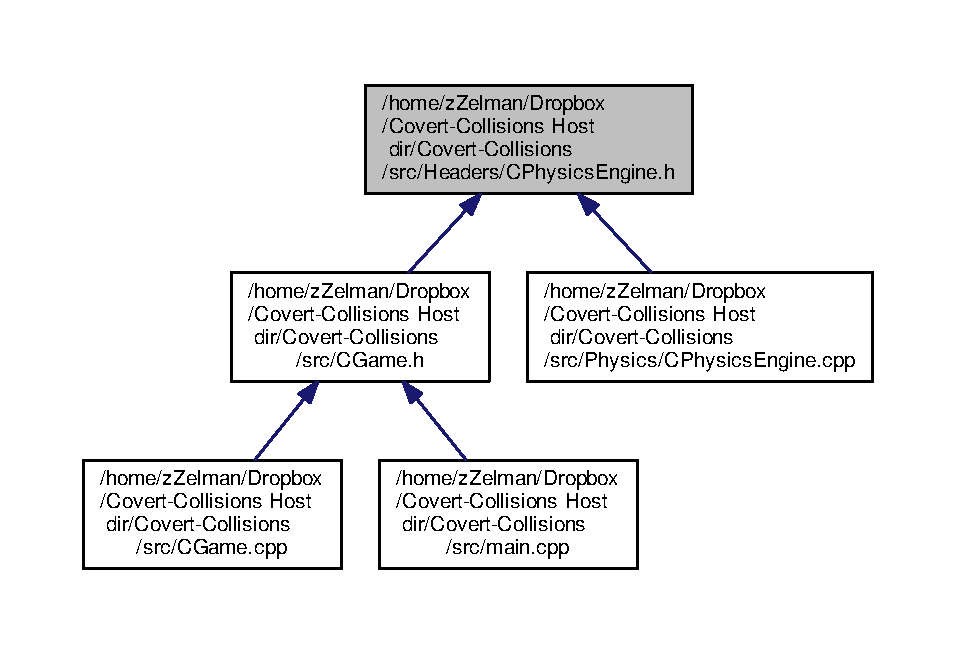
\includegraphics[width=350pt]{CPhysicsEngine_8h__dep__incl}
\end{center}
\end{figure}
\subsection*{Classes}
\begin{DoxyCompactItemize}
\item 
class \hyperlink{classCPhysicsEngine}{C\-Physics\-Engine}
\begin{DoxyCompactList}\small\item\em Module of the game engine that is responsible for\-: resolving collisions and updating physics data within objects. \end{DoxyCompactList}\end{DoxyCompactItemize}

\hypertarget{CPlayer_8h}{\section{/home/z\-Zelman/\-Dropbox/\-Covert-\/\-Collisions Host dir/\-Covert-\/\-Collisions/src/\-Headers/\-C\-Player.h File Reference}
\label{CPlayer_8h}\index{/home/z\-Zelman/\-Dropbox/\-Covert-\/\-Collisions Host dir/\-Covert-\/\-Collisions/src/\-Headers/\-C\-Player.\-h@{/home/z\-Zelman/\-Dropbox/\-Covert-\/\-Collisions Host dir/\-Covert-\/\-Collisions/src/\-Headers/\-C\-Player.\-h}}
}
{\ttfamily \#include \char`\"{}include\-\_\-sfml.\-h\char`\"{}}\\*
{\ttfamily \#include \char`\"{}A\-Renderable.\-h\char`\"{}}\\*
{\ttfamily \#include \char`\"{}A\-Update.\-h\char`\"{}}\\*
{\ttfamily \#include \char`\"{}A\-User\-Input.\-h\char`\"{}}\\*
{\ttfamily \#include \char`\"{}C\-Texture.\-h\char`\"{}}\\*
{\ttfamily \#include \char`\"{}D\-Physics.\-h\char`\"{}}\\*
Include dependency graph for C\-Player.\-h\-:\nopagebreak
\begin{figure}[H]
\begin{center}
\leavevmode
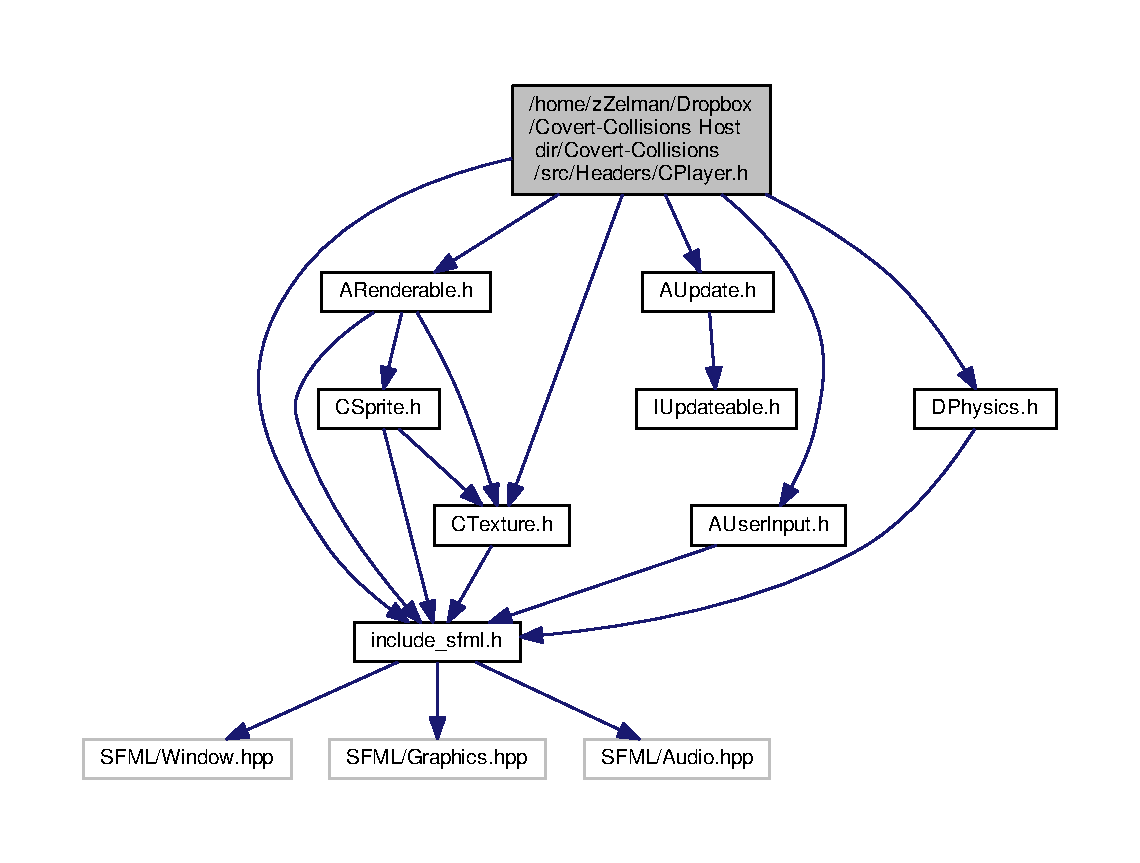
\includegraphics[width=350pt]{CPlayer_8h__incl}
\end{center}
\end{figure}
This graph shows which files directly or indirectly include this file\-:\nopagebreak
\begin{figure}[H]
\begin{center}
\leavevmode
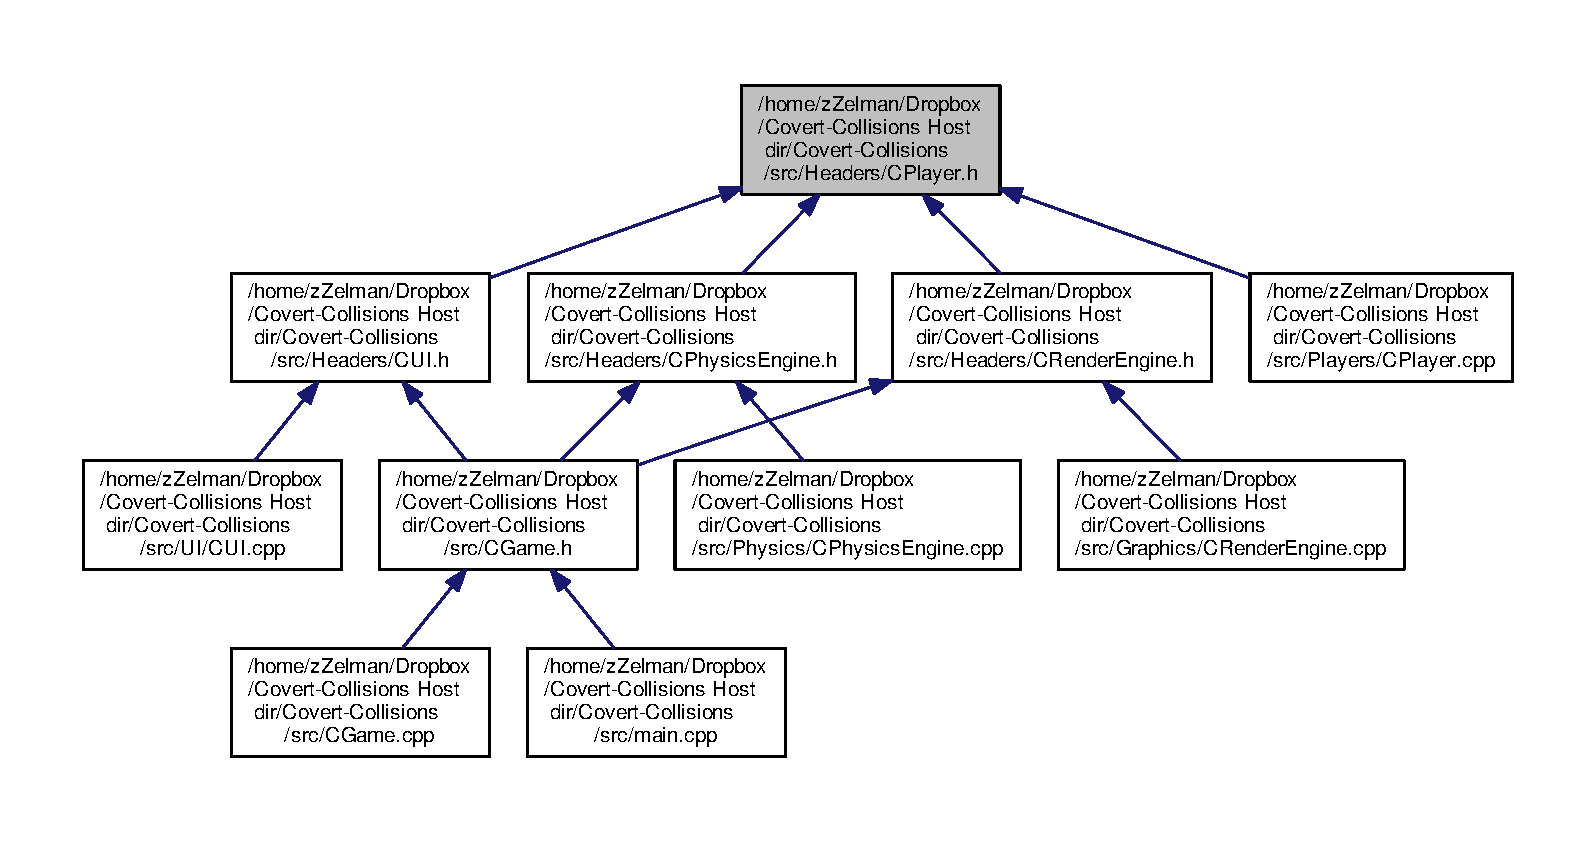
\includegraphics[width=350pt]{CPlayer_8h__dep__incl}
\end{center}
\end{figure}
\subsection*{Classes}
\begin{DoxyCompactItemize}
\item 
class \hyperlink{classCPlayer}{C\-Player}
\begin{DoxyCompactList}\small\item\em Base class of each individual player. \end{DoxyCompactList}\end{DoxyCompactItemize}

\hypertarget{CRenderEngine_8h}{\section{/home/z\-Zelman/\-Dropbox/\-Covert-\/\-Collisions Host dir/\-Covert-\/\-Collisions/src/\-Headers/\-C\-Render\-Engine.h File Reference}
\label{CRenderEngine_8h}\index{/home/z\-Zelman/\-Dropbox/\-Covert-\/\-Collisions Host dir/\-Covert-\/\-Collisions/src/\-Headers/\-C\-Render\-Engine.\-h@{/home/z\-Zelman/\-Dropbox/\-Covert-\/\-Collisions Host dir/\-Covert-\/\-Collisions/src/\-Headers/\-C\-Render\-Engine.\-h}}
}
{\ttfamily \#include \char`\"{}include\-\_\-sfml.\-h\char`\"{}}\\*
{\ttfamily \#include \char`\"{}A\-Renderable.\-h\char`\"{}}\\*
{\ttfamily \#include \char`\"{}C\-Tile\-\_\-\-Container.\-h\char`\"{}}\\*
{\ttfamily \#include \char`\"{}C\-Player.\-h\char`\"{}}\\*
{\ttfamily \#include $<$list$>$}\\*
Include dependency graph for C\-Render\-Engine.\-h\-:\nopagebreak
\begin{figure}[H]
\begin{center}
\leavevmode
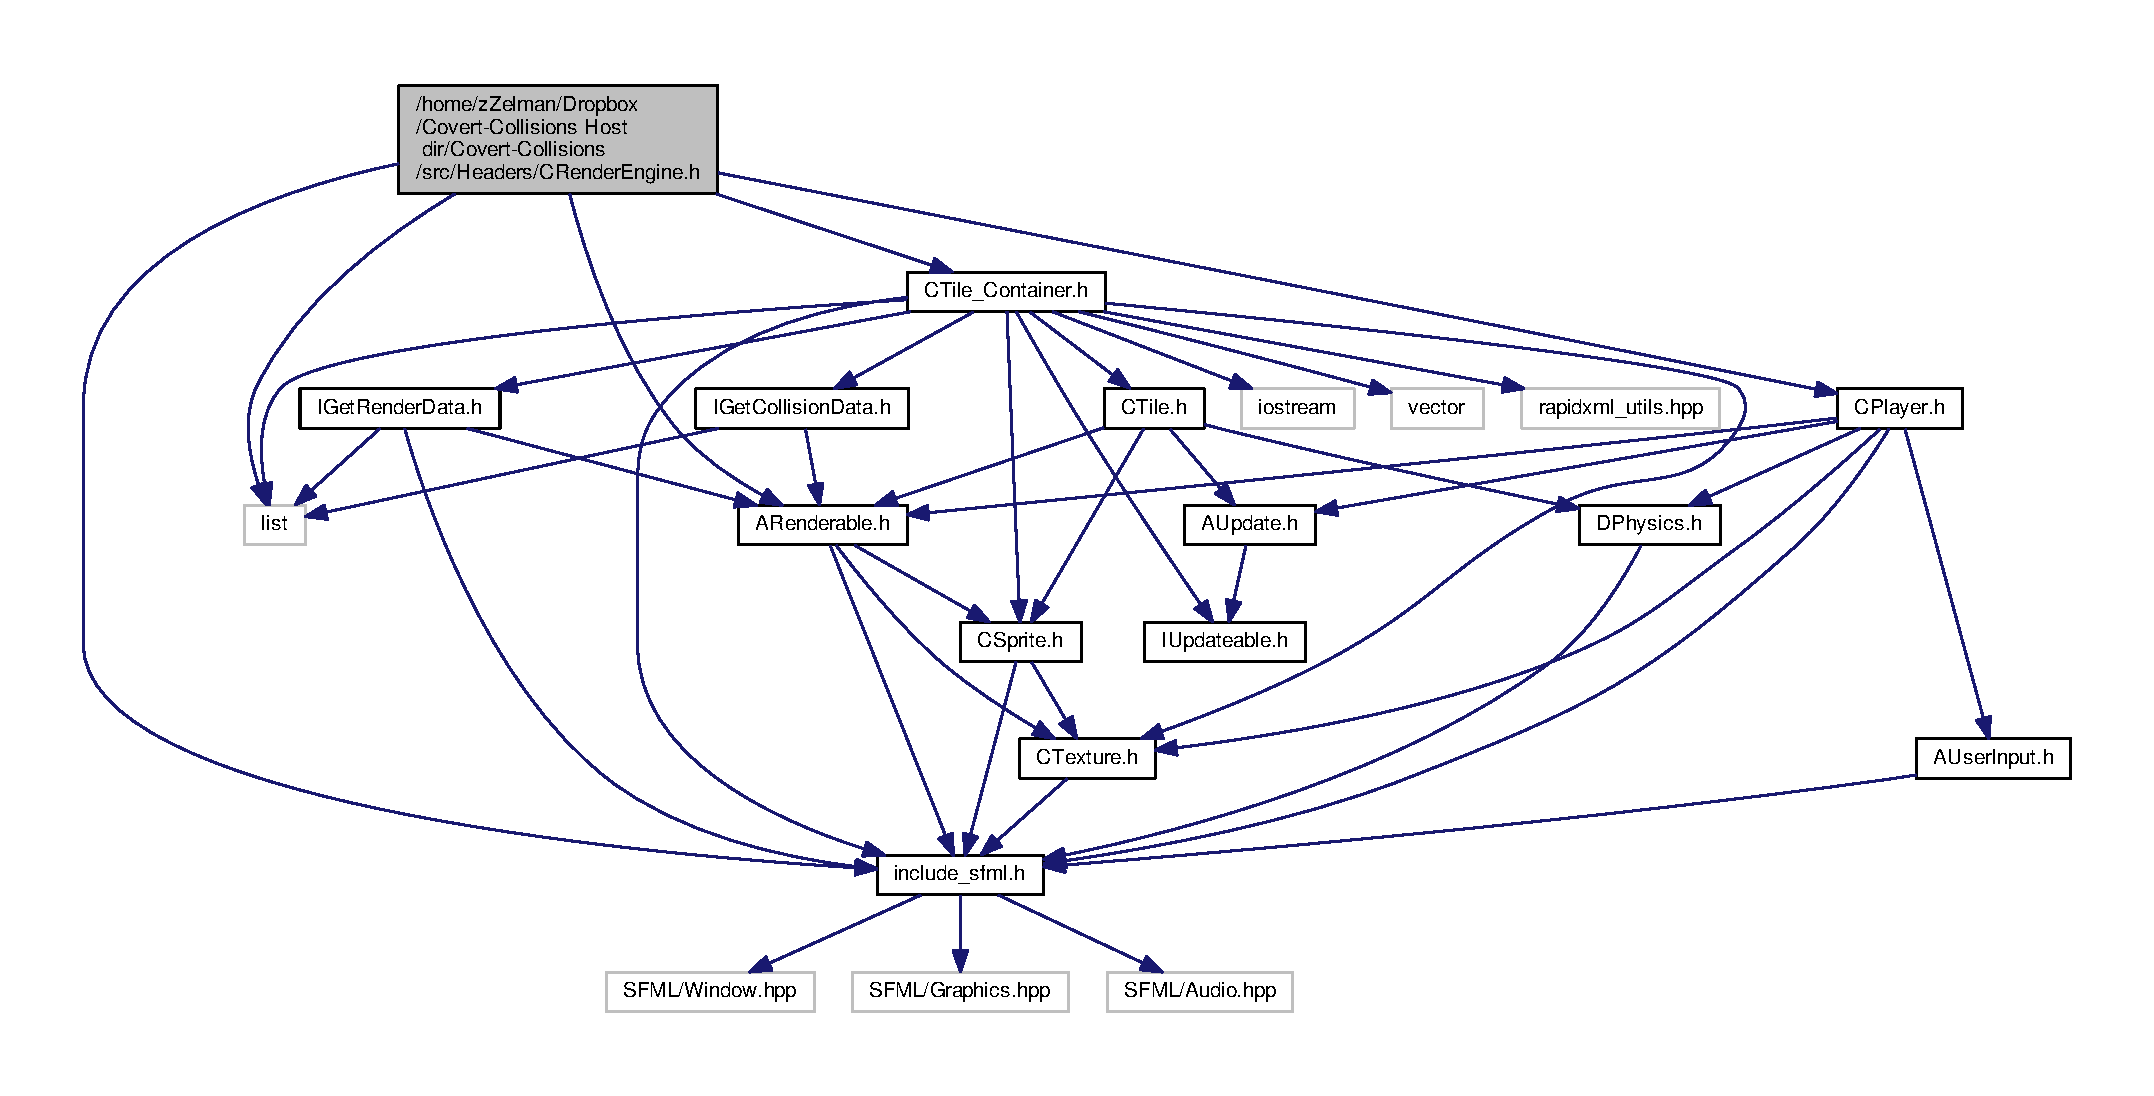
\includegraphics[width=350pt]{CRenderEngine_8h__incl}
\end{center}
\end{figure}
This graph shows which files directly or indirectly include this file\-:\nopagebreak
\begin{figure}[H]
\begin{center}
\leavevmode
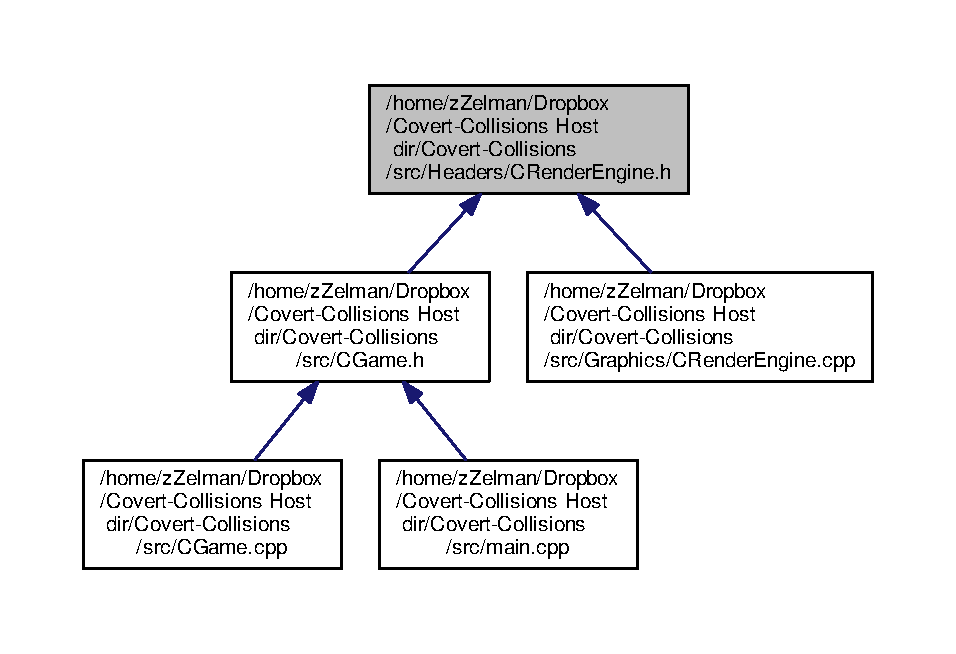
\includegraphics[width=350pt]{CRenderEngine_8h__dep__incl}
\end{center}
\end{figure}
\subsection*{Classes}
\begin{DoxyCompactItemize}
\item 
class \hyperlink{classCRenderEngine}{C\-Render\-Engine}
\begin{DoxyCompactList}\small\item\em Module of the game engine that is responsible for rendering all \hyperlink{classARenderable}{A\-Renderable} game objects in an ordered fashion. \end{DoxyCompactList}\end{DoxyCompactItemize}

\hypertarget{CSprite_8h}{\section{/home/z\-Zelman/\-Dropbox/\-Covert-\/\-Collisions Host dir/\-Covert-\/\-Collisions/src/\-Headers/\-C\-Sprite.h File Reference}
\label{CSprite_8h}\index{/home/z\-Zelman/\-Dropbox/\-Covert-\/\-Collisions Host dir/\-Covert-\/\-Collisions/src/\-Headers/\-C\-Sprite.\-h@{/home/z\-Zelman/\-Dropbox/\-Covert-\/\-Collisions Host dir/\-Covert-\/\-Collisions/src/\-Headers/\-C\-Sprite.\-h}}
}
{\ttfamily \#include \char`\"{}include\-\_\-sfml.\-h\char`\"{}}\\*
{\ttfamily \#include \char`\"{}C\-Texture.\-h\char`\"{}}\\*
Include dependency graph for C\-Sprite.\-h\-:\nopagebreak
\begin{figure}[H]
\begin{center}
\leavevmode
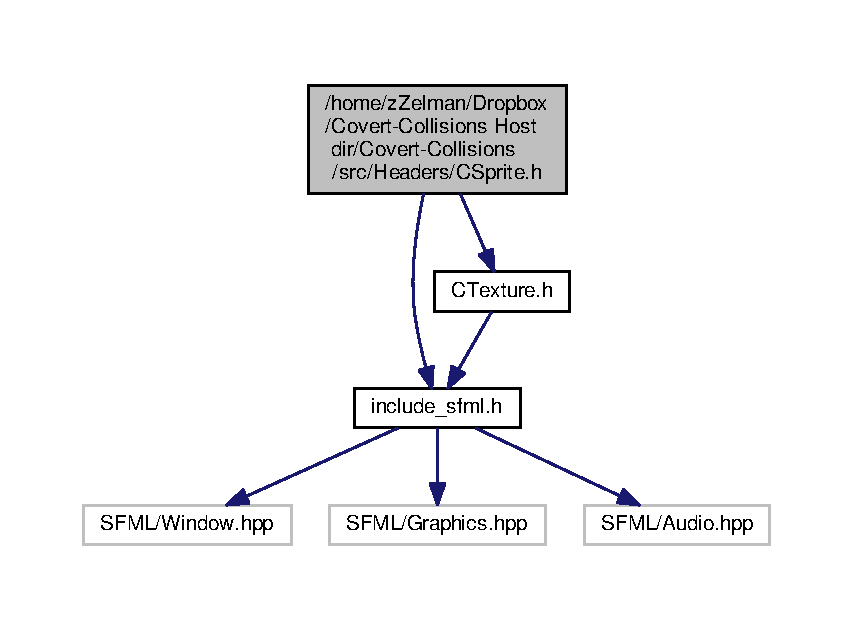
\includegraphics[width=350pt]{CSprite_8h__incl}
\end{center}
\end{figure}
This graph shows which files directly or indirectly include this file\-:\nopagebreak
\begin{figure}[H]
\begin{center}
\leavevmode
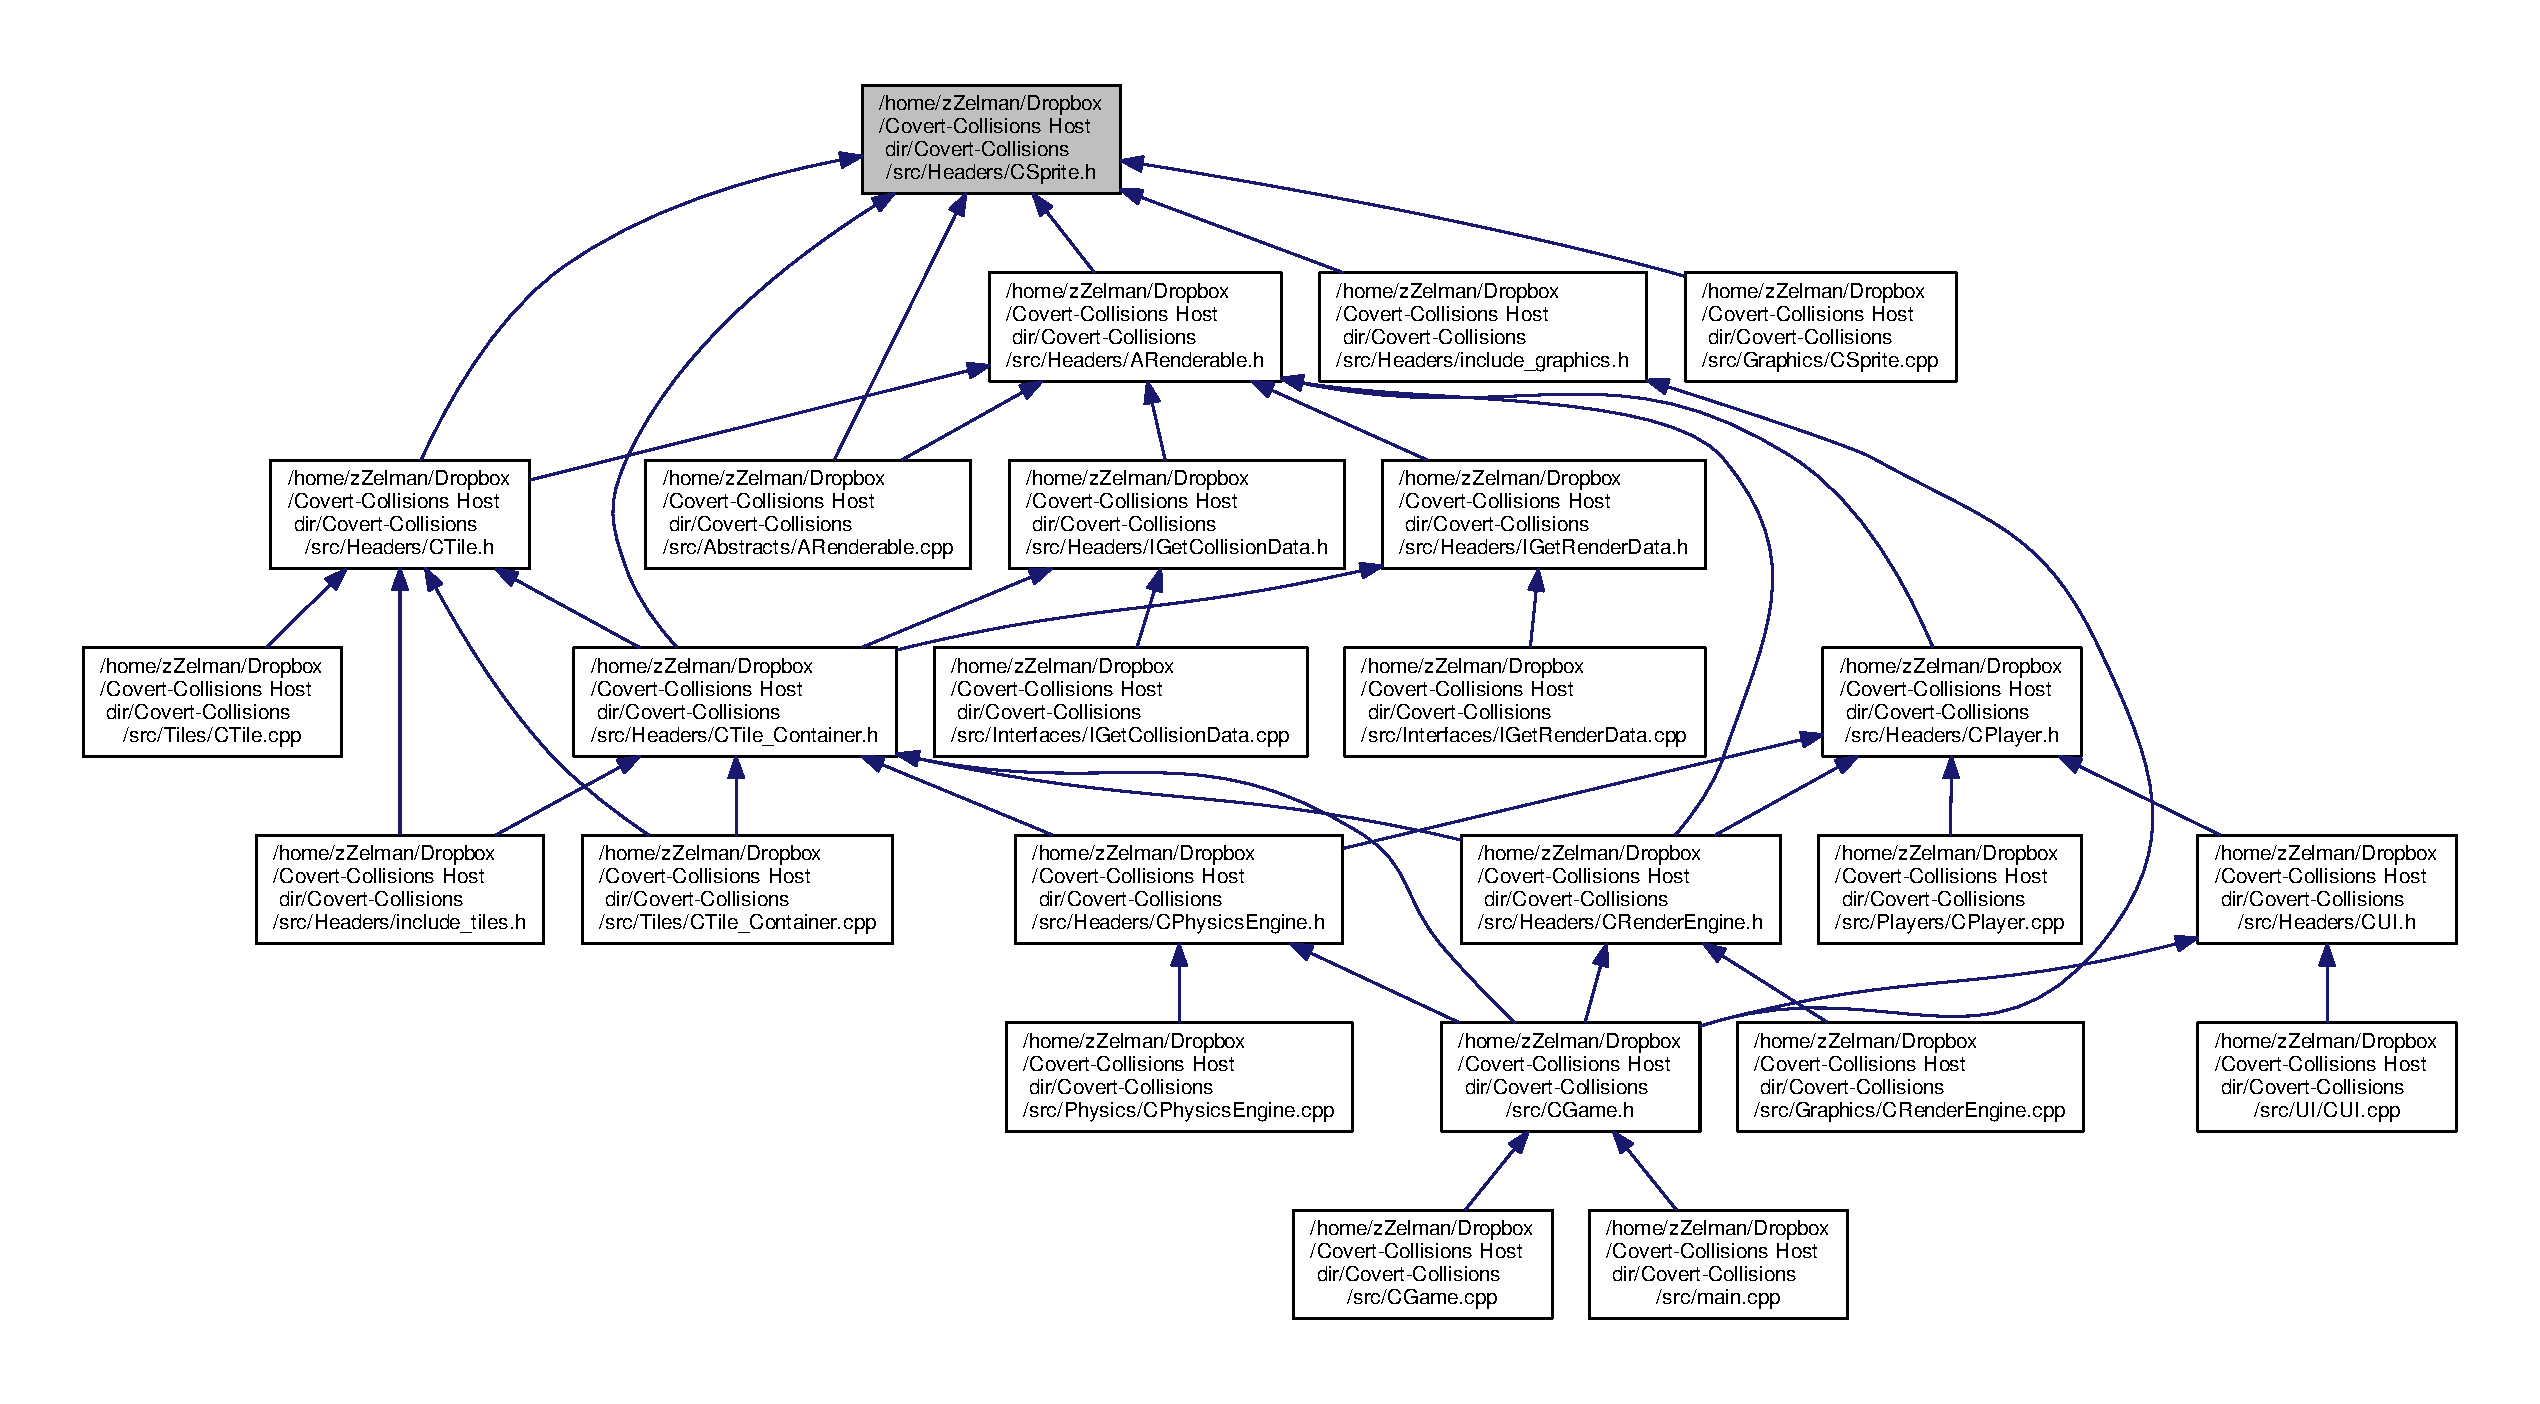
\includegraphics[width=350pt]{CSprite_8h__dep__incl}
\end{center}
\end{figure}
\subsection*{Classes}
\begin{DoxyCompactItemize}
\item 
class \hyperlink{classCSprite}{C\-Sprite}
\begin{DoxyCompactList}\small\item\em Wrapper class for S\-F\-M\-L 2.\-1 Sprite. \end{DoxyCompactList}\end{DoxyCompactItemize}

\hypertarget{CTexture_8h}{\section{/home/z\-Zelman/\-Dropbox/\-Covert-\/\-Collisions Host dir/\-Covert-\/\-Collisions/src/\-Headers/\-C\-Texture.h File Reference}
\label{CTexture_8h}\index{/home/z\-Zelman/\-Dropbox/\-Covert-\/\-Collisions Host dir/\-Covert-\/\-Collisions/src/\-Headers/\-C\-Texture.\-h@{/home/z\-Zelman/\-Dropbox/\-Covert-\/\-Collisions Host dir/\-Covert-\/\-Collisions/src/\-Headers/\-C\-Texture.\-h}}
}
{\ttfamily \#include \char`\"{}include\-\_\-sfml.\-h\char`\"{}}\\*
Include dependency graph for C\-Texture.\-h\-:\nopagebreak
\begin{figure}[H]
\begin{center}
\leavevmode
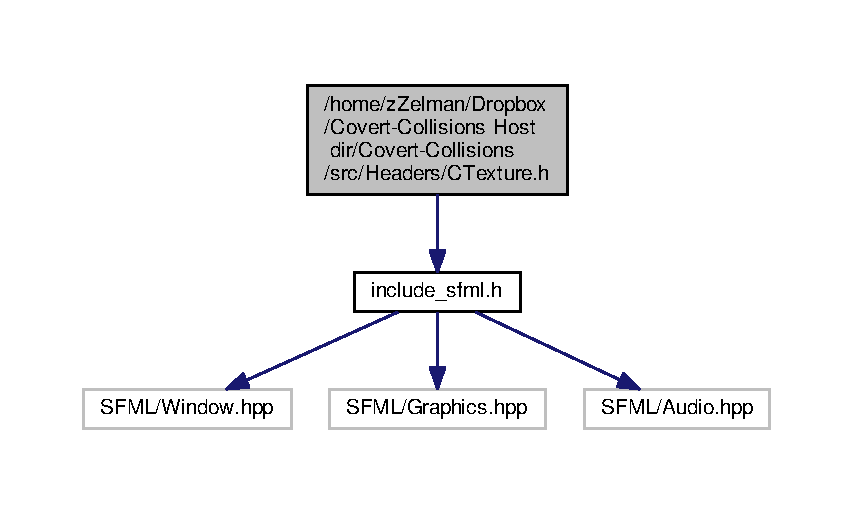
\includegraphics[width=350pt]{CTexture_8h__incl}
\end{center}
\end{figure}
This graph shows which files directly or indirectly include this file\-:\nopagebreak
\begin{figure}[H]
\begin{center}
\leavevmode
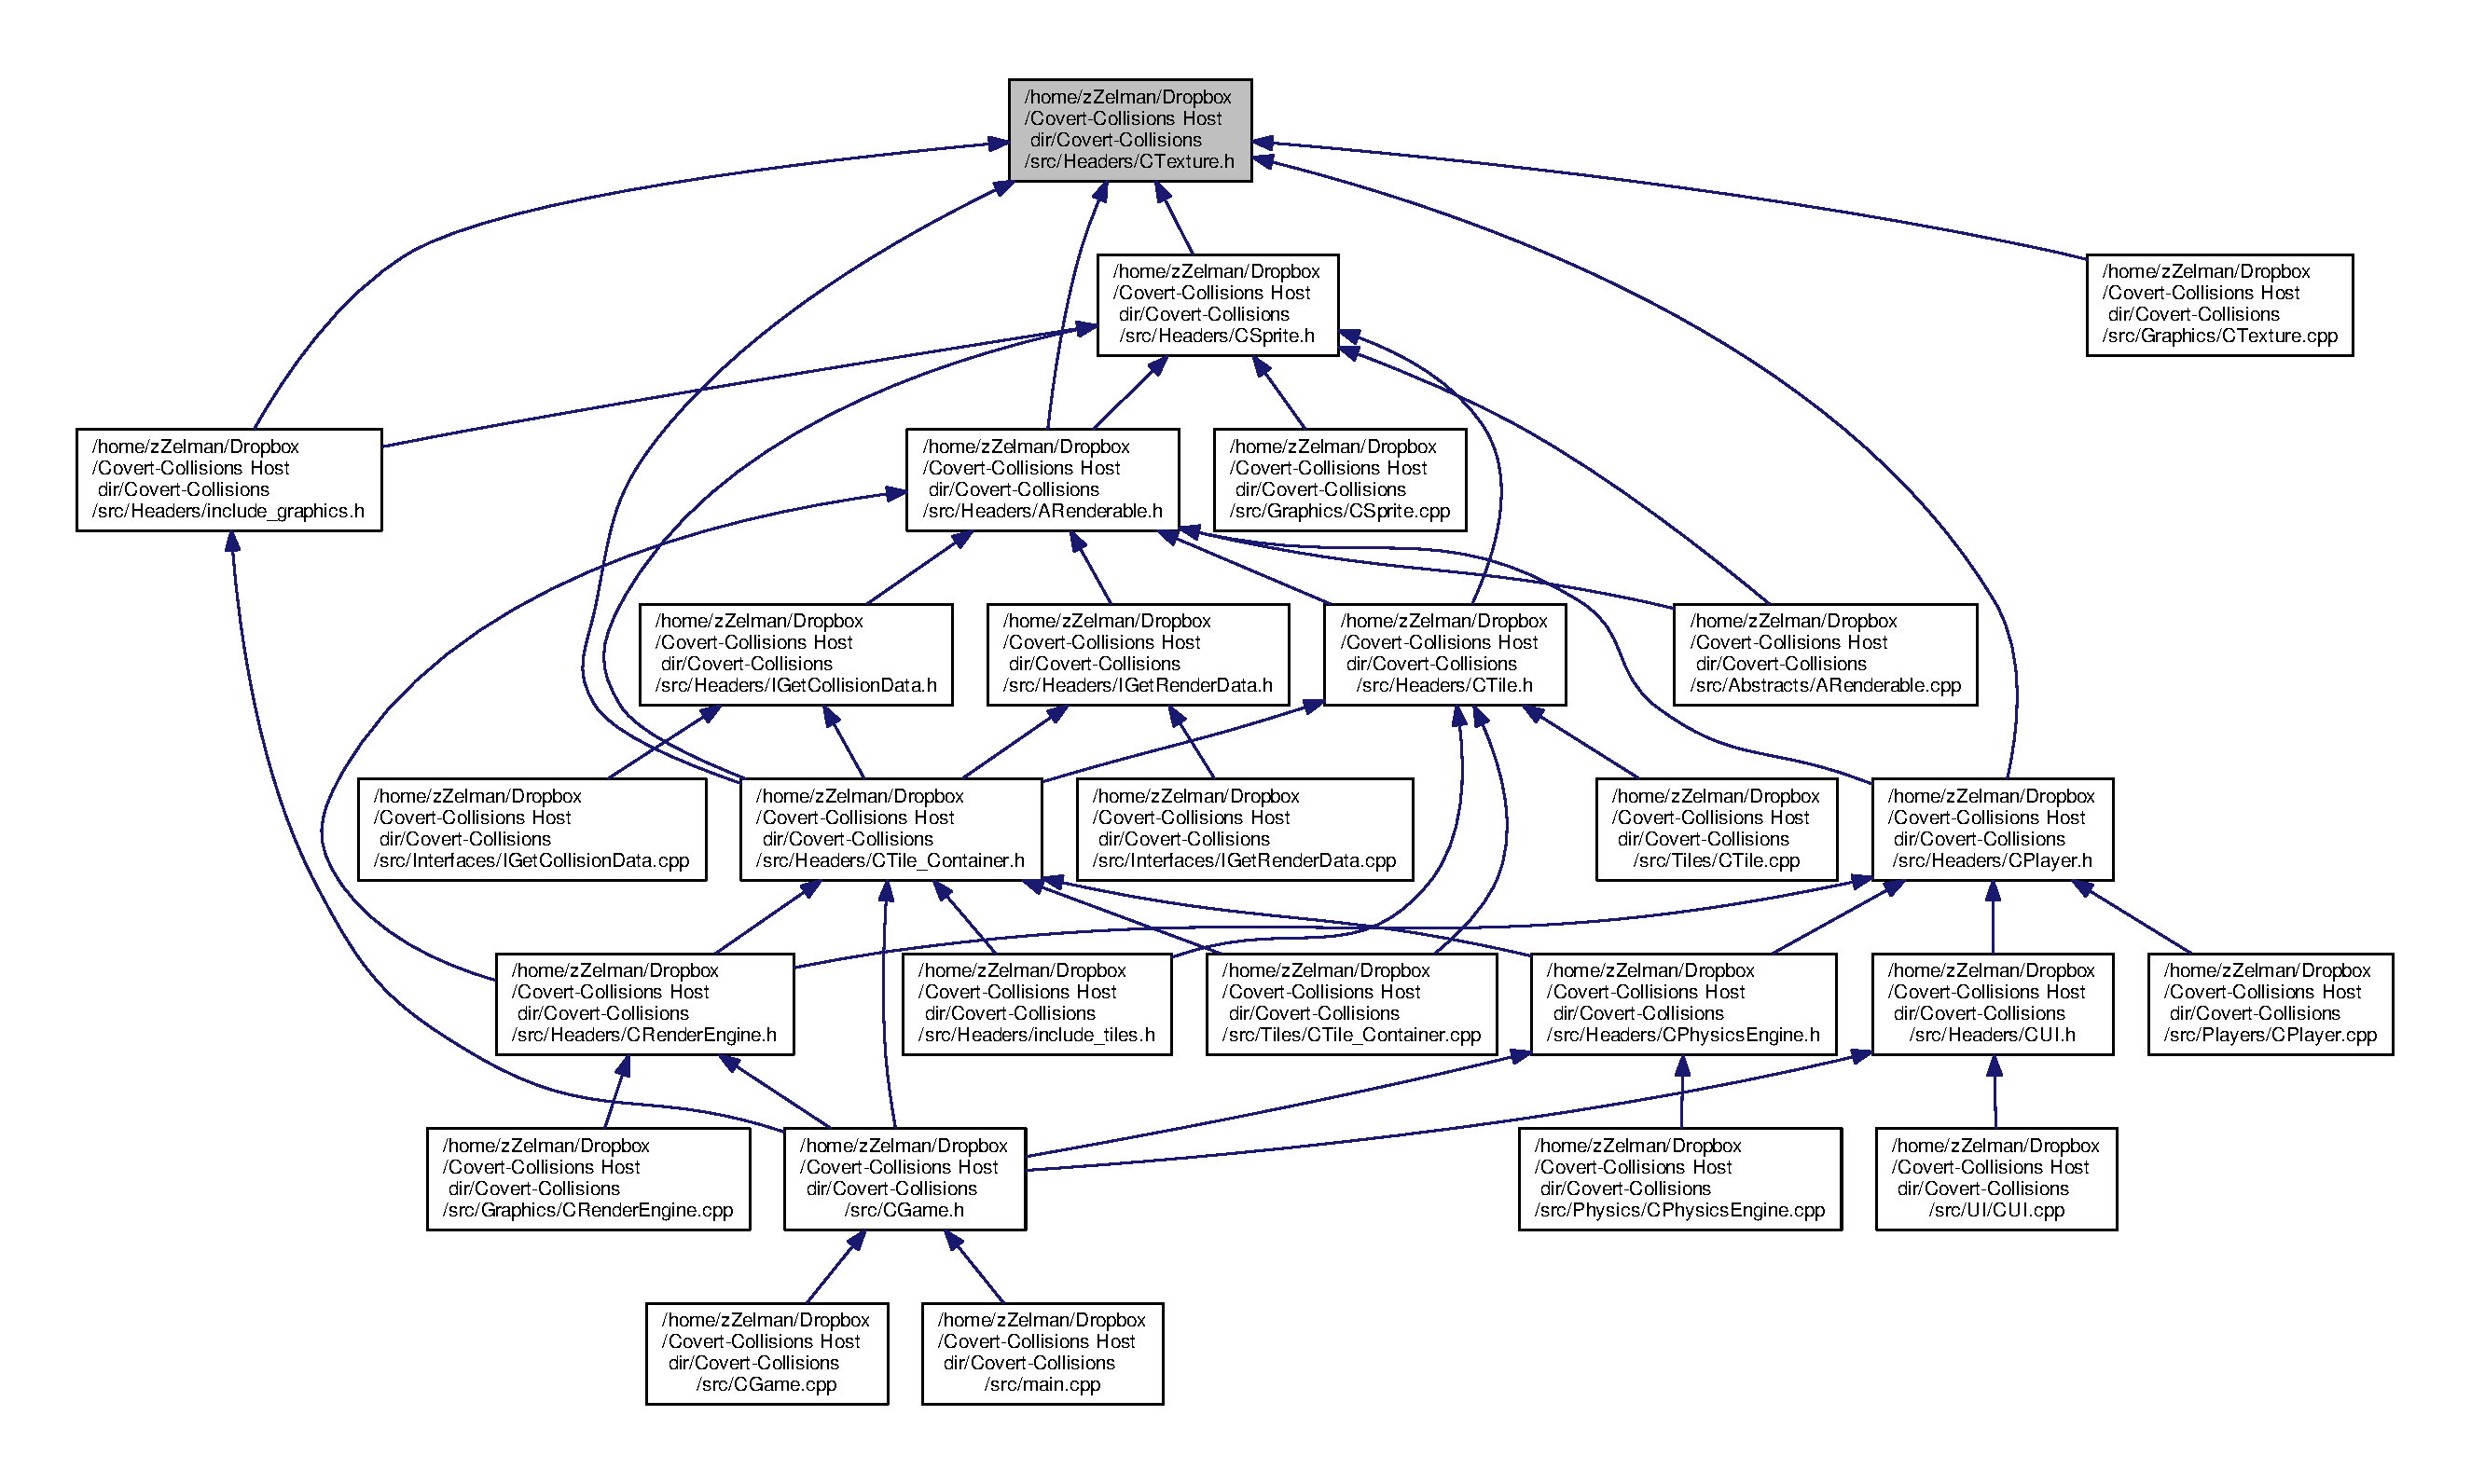
\includegraphics[width=350pt]{CTexture_8h__dep__incl}
\end{center}
\end{figure}
\subsection*{Classes}
\begin{DoxyCompactItemize}
\item 
class \hyperlink{classCTexture}{C\-Texture}
\begin{DoxyCompactList}\small\item\em Wrapper class for S\-F\-M\-L 2.\-1 Texture. \end{DoxyCompactList}\end{DoxyCompactItemize}

\hypertarget{CTile_8h}{\section{/home/z\-Zelman/\-Dropbox/\-Covert-\/\-Collisions Host dir/\-Covert-\/\-Collisions/src/\-Headers/\-C\-Tile.h File Reference}
\label{CTile_8h}\index{/home/z\-Zelman/\-Dropbox/\-Covert-\/\-Collisions Host dir/\-Covert-\/\-Collisions/src/\-Headers/\-C\-Tile.\-h@{/home/z\-Zelman/\-Dropbox/\-Covert-\/\-Collisions Host dir/\-Covert-\/\-Collisions/src/\-Headers/\-C\-Tile.\-h}}
}
{\ttfamily \#include \char`\"{}A\-Renderable.\-h\char`\"{}}\\*
{\ttfamily \#include \char`\"{}A\-Update.\-h\char`\"{}}\\*
{\ttfamily \#include \char`\"{}D\-Physics.\-h\char`\"{}}\\*
{\ttfamily \#include \char`\"{}C\-Sprite.\-h\char`\"{}}\\*
Include dependency graph for C\-Tile.\-h\-:\nopagebreak
\begin{figure}[H]
\begin{center}
\leavevmode
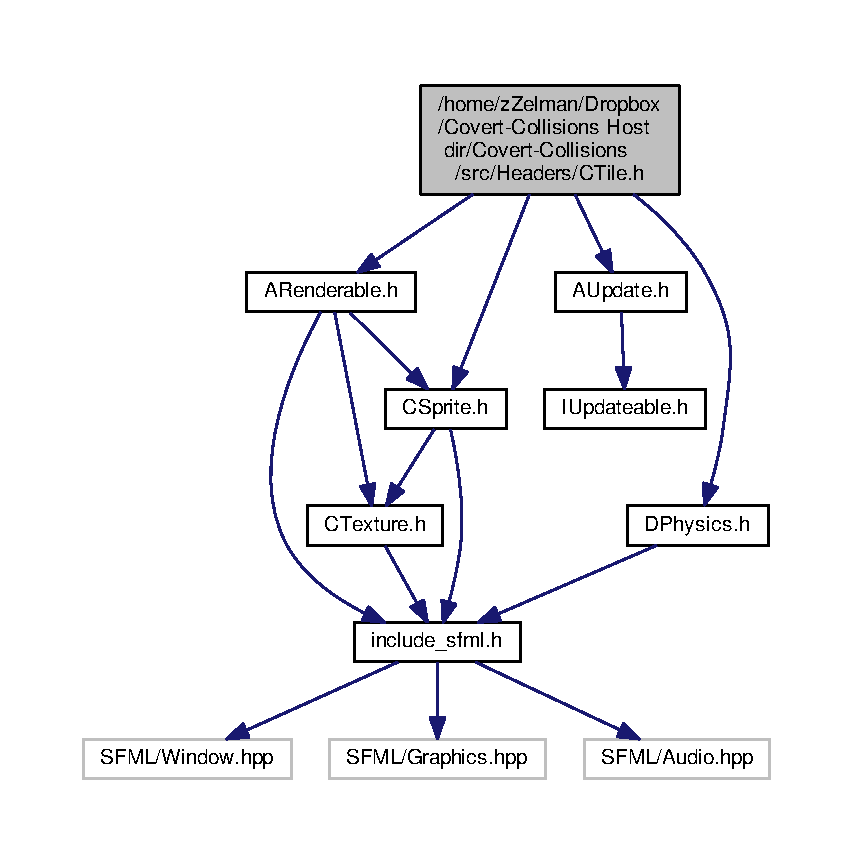
\includegraphics[width=350pt]{CTile_8h__incl}
\end{center}
\end{figure}
This graph shows which files directly or indirectly include this file\-:\nopagebreak
\begin{figure}[H]
\begin{center}
\leavevmode
\includegraphics[width=350pt]{CTile_8h__dep__incl}
\end{center}
\end{figure}
\subsection*{Classes}
\begin{DoxyCompactItemize}
\item 
class \hyperlink{classCTile}{C\-Tile}
\begin{DoxyCompactList}\small\item\em Rectangle of rigid space that is a rendered platform or wall. \end{DoxyCompactList}\end{DoxyCompactItemize}

\hypertarget{CTile__Container_8h}{\section{/home/z\-Zelman/\-Dropbox/\-Covert-\/\-Collisions Host dir/\-Covert-\/\-Collisions/src/\-Headers/\-C\-Tile\-\_\-\-Container.h File Reference}
\label{CTile__Container_8h}\index{/home/z\-Zelman/\-Dropbox/\-Covert-\/\-Collisions Host dir/\-Covert-\/\-Collisions/src/\-Headers/\-C\-Tile\-\_\-\-Container.\-h@{/home/z\-Zelman/\-Dropbox/\-Covert-\/\-Collisions Host dir/\-Covert-\/\-Collisions/src/\-Headers/\-C\-Tile\-\_\-\-Container.\-h}}
}
{\ttfamily \#include \char`\"{}include\-\_\-sfml.\-h\char`\"{}}\\*
{\ttfamily \#include \char`\"{}I\-Updateable.\-h\char`\"{}}\\*
{\ttfamily \#include \char`\"{}C\-Texture.\-h\char`\"{}}\\*
{\ttfamily \#include \char`\"{}C\-Sprite.\-h\char`\"{}}\\*
{\ttfamily \#include $<$iostream$>$}\\*
{\ttfamily \#include $<$vector$>$}\\*
{\ttfamily \#include \char`\"{}rapidxml\-\_\-utils.\-hpp\char`\"{}}\\*
{\ttfamily \#include \char`\"{}C\-Tile.\-h\char`\"{}}\\*
{\ttfamily \#include \char`\"{}I\-Get\-Collision\-Data.\-h\char`\"{}}\\*
{\ttfamily \#include \char`\"{}I\-Get\-Render\-Data.\-h\char`\"{}}\\*
{\ttfamily \#include $<$list$>$}\\*
Include dependency graph for C\-Tile\-\_\-\-Container.\-h\-:\nopagebreak
\begin{figure}[H]
\begin{center}
\leavevmode
\includegraphics[width=350pt]{CTile__Container_8h__incl}
\end{center}
\end{figure}
This graph shows which files directly or indirectly include this file\-:\nopagebreak
\begin{figure}[H]
\begin{center}
\leavevmode
\includegraphics[width=350pt]{CTile__Container_8h__dep__incl}
\end{center}
\end{figure}
\subsection*{Classes}
\begin{DoxyCompactItemize}
\item 
class \hyperlink{classCTile__Container}{C\-Tile\-\_\-\-Container}
\begin{DoxyCompactList}\small\item\em T\-O\-D\-O\-: This object needs to be re-\/writen to expand functionality. \end{DoxyCompactList}\end{DoxyCompactItemize}

\hypertarget{CUI_8h}{\section{/home/z\-Zelman/\-Dropbox/\-Covert-\/\-Collisions Host dir/\-Covert-\/\-Collisions/src/\-Headers/\-C\-U\-I.h File Reference}
\label{CUI_8h}\index{/home/z\-Zelman/\-Dropbox/\-Covert-\/\-Collisions Host dir/\-Covert-\/\-Collisions/src/\-Headers/\-C\-U\-I.\-h@{/home/z\-Zelman/\-Dropbox/\-Covert-\/\-Collisions Host dir/\-Covert-\/\-Collisions/src/\-Headers/\-C\-U\-I.\-h}}
}
{\ttfamily \#include \char`\"{}include\-\_\-sfml.\-h\char`\"{}}\\*
{\ttfamily \#include \char`\"{}C\-Player.\-h\char`\"{}}\\*
{\ttfamily \#include \char`\"{}I\-Updateable.\-h\char`\"{}}\\*
{\ttfamily \#include \char`\"{}A\-User\-Input.\-h\char`\"{}}\\*
Include dependency graph for C\-U\-I.\-h\-:\nopagebreak
\begin{figure}[H]
\begin{center}
\leavevmode
\includegraphics[width=350pt]{CUI_8h__incl}
\end{center}
\end{figure}
This graph shows which files directly or indirectly include this file\-:\nopagebreak
\begin{figure}[H]
\begin{center}
\leavevmode
\includegraphics[width=350pt]{CUI_8h__dep__incl}
\end{center}
\end{figure}
\subsection*{Classes}
\begin{DoxyCompactItemize}
\item 
class \hyperlink{classCUI}{C\-U\-I}
\begin{DoxyCompactList}\small\item\em 'Parses' user events, as well as keeps Bookkeeping information on several user states. \end{DoxyCompactList}\end{DoxyCompactItemize}

\hypertarget{DPhysics_8h}{\section{/home/z\-Zelman/\-Dropbox/\-Covert-\/\-Collisions Host dir/\-Covert-\/\-Collisions/src/\-Headers/\-D\-Physics.h File Reference}
\label{DPhysics_8h}\index{/home/z\-Zelman/\-Dropbox/\-Covert-\/\-Collisions Host dir/\-Covert-\/\-Collisions/src/\-Headers/\-D\-Physics.\-h@{/home/z\-Zelman/\-Dropbox/\-Covert-\/\-Collisions Host dir/\-Covert-\/\-Collisions/src/\-Headers/\-D\-Physics.\-h}}
}
{\ttfamily \#include \char`\"{}include\-\_\-sfml.\-h\char`\"{}}\\*
Include dependency graph for D\-Physics.\-h\-:\nopagebreak
\begin{figure}[H]
\begin{center}
\leavevmode
\includegraphics[width=350pt]{DPhysics_8h__incl}
\end{center}
\end{figure}
This graph shows which files directly or indirectly include this file\-:\nopagebreak
\begin{figure}[H]
\begin{center}
\leavevmode
\includegraphics[width=350pt]{DPhysics_8h__dep__incl}
\end{center}
\end{figure}
\subsection*{Classes}
\begin{DoxyCompactItemize}
\item 
class \hyperlink{classDPhysics}{D\-Physics}
\begin{DoxyCompactList}\small\item\em Base class holder of pertinent physics information within a \hyperlink{structDPhysics_1_1SPhysics}{S\-Physics}. \end{DoxyCompactList}\item 
struct \hyperlink{structDPhysics_1_1SPhysics}{D\-Physics\-::\-S\-Physics}
\begin{DoxyCompactList}\small\item\em Physics data. \end{DoxyCompactList}\end{DoxyCompactItemize}

\hypertarget{IGetCollisionData_8h}{\section{/home/z\-Zelman/\-Dropbox/\-Covert-\/\-Collisions Host dir/\-Covert-\/\-Collisions/src/\-Headers/\-I\-Get\-Collision\-Data.h File Reference}
\label{IGetCollisionData_8h}\index{/home/z\-Zelman/\-Dropbox/\-Covert-\/\-Collisions Host dir/\-Covert-\/\-Collisions/src/\-Headers/\-I\-Get\-Collision\-Data.\-h@{/home/z\-Zelman/\-Dropbox/\-Covert-\/\-Collisions Host dir/\-Covert-\/\-Collisions/src/\-Headers/\-I\-Get\-Collision\-Data.\-h}}
}
{\ttfamily \#include $<$list$>$}\\*
{\ttfamily \#include \char`\"{}A\-Renderable.\-h\char`\"{}}\\*
Include dependency graph for I\-Get\-Collision\-Data.\-h\-:\nopagebreak
\begin{figure}[H]
\begin{center}
\leavevmode
\includegraphics[width=350pt]{IGetCollisionData_8h__incl}
\end{center}
\end{figure}
This graph shows which files directly or indirectly include this file\-:\nopagebreak
\begin{figure}[H]
\begin{center}
\leavevmode
\includegraphics[width=350pt]{IGetCollisionData_8h__dep__incl}
\end{center}
\end{figure}
\subsection*{Classes}
\begin{DoxyCompactItemize}
\item 
class \hyperlink{classIGetCollisionData}{I\-Get\-Collision\-Data}
\begin{DoxyCompactList}\small\item\em A common interface from pulling relevant collision data from objects. \end{DoxyCompactList}\end{DoxyCompactItemize}

\hypertarget{IGetRenderData_8h}{\section{/home/z\-Zelman/\-Dropbox/\-Covert-\/\-Collisions Host dir/\-Covert-\/\-Collisions/src/\-Headers/\-I\-Get\-Render\-Data.h File Reference}
\label{IGetRenderData_8h}\index{/home/z\-Zelman/\-Dropbox/\-Covert-\/\-Collisions Host dir/\-Covert-\/\-Collisions/src/\-Headers/\-I\-Get\-Render\-Data.\-h@{/home/z\-Zelman/\-Dropbox/\-Covert-\/\-Collisions Host dir/\-Covert-\/\-Collisions/src/\-Headers/\-I\-Get\-Render\-Data.\-h}}
}
{\ttfamily \#include \char`\"{}include\-\_\-sfml.\-h\char`\"{}}\\*
{\ttfamily \#include \char`\"{}A\-Renderable.\-h\char`\"{}}\\*
{\ttfamily \#include $<$list$>$}\\*
Include dependency graph for I\-Get\-Render\-Data.\-h\-:\nopagebreak
\begin{figure}[H]
\begin{center}
\leavevmode
\includegraphics[width=350pt]{IGetRenderData_8h__incl}
\end{center}
\end{figure}
This graph shows which files directly or indirectly include this file\-:\nopagebreak
\begin{figure}[H]
\begin{center}
\leavevmode
\includegraphics[width=350pt]{IGetRenderData_8h__dep__incl}
\end{center}
\end{figure}
\subsection*{Classes}
\begin{DoxyCompactItemize}
\item 
class \hyperlink{classIGetRenderData}{I\-Get\-Render\-Data}
\begin{DoxyCompactList}\small\item\em A common interface for pulling relavent rendering information out of objects. \end{DoxyCompactList}\end{DoxyCompactItemize}

\hypertarget{include__graphics_8h}{\section{/home/z\-Zelman/\-Dropbox/\-Covert-\/\-Collisions Host dir/\-Covert-\/\-Collisions/src/\-Headers/include\-\_\-graphics.h File Reference}
\label{include__graphics_8h}\index{/home/z\-Zelman/\-Dropbox/\-Covert-\/\-Collisions Host dir/\-Covert-\/\-Collisions/src/\-Headers/include\-\_\-graphics.\-h@{/home/z\-Zelman/\-Dropbox/\-Covert-\/\-Collisions Host dir/\-Covert-\/\-Collisions/src/\-Headers/include\-\_\-graphics.\-h}}
}
{\ttfamily \#include \char`\"{}C\-Sprite.\-h\char`\"{}}\\*
{\ttfamily \#include \char`\"{}C\-Texture.\-h\char`\"{}}\\*
Include dependency graph for include\-\_\-graphics.\-h\-:\nopagebreak
\begin{figure}[H]
\begin{center}
\leavevmode
\includegraphics[width=350pt]{include__graphics_8h__incl}
\end{center}
\end{figure}
This graph shows which files directly or indirectly include this file\-:\nopagebreak
\begin{figure}[H]
\begin{center}
\leavevmode
\includegraphics[width=346pt]{include__graphics_8h__dep__incl}
\end{center}
\end{figure}

\hypertarget{include__sfml_8h}{\section{/home/z\-Zelman/\-Dropbox/\-Covert-\/\-Collisions Host dir/\-Covert-\/\-Collisions/src/\-Headers/include\-\_\-sfml.h File Reference}
\label{include__sfml_8h}\index{/home/z\-Zelman/\-Dropbox/\-Covert-\/\-Collisions Host dir/\-Covert-\/\-Collisions/src/\-Headers/include\-\_\-sfml.\-h@{/home/z\-Zelman/\-Dropbox/\-Covert-\/\-Collisions Host dir/\-Covert-\/\-Collisions/src/\-Headers/include\-\_\-sfml.\-h}}
}
{\ttfamily \#include $<$S\-F\-M\-L/\-Window.\-hpp$>$}\\*
{\ttfamily \#include $<$S\-F\-M\-L/\-Graphics.\-hpp$>$}\\*
{\ttfamily \#include $<$S\-F\-M\-L/\-Audio.\-hpp$>$}\\*
Include dependency graph for include\-\_\-sfml.\-h\-:\nopagebreak
\begin{figure}[H]
\begin{center}
\leavevmode
\includegraphics[width=350pt]{include__sfml_8h__incl}
\end{center}
\end{figure}
This graph shows which files directly or indirectly include this file\-:\nopagebreak
\begin{figure}[H]
\begin{center}
\leavevmode
\includegraphics[width=350pt]{include__sfml_8h__dep__incl}
\end{center}
\end{figure}

\hypertarget{include__tiles_8h}{\section{/home/z\-Zelman/\-Dropbox/\-Covert-\/\-Collisions Host dir/\-Covert-\/\-Collisions/src/\-Headers/include\-\_\-tiles.h File Reference}
\label{include__tiles_8h}\index{/home/z\-Zelman/\-Dropbox/\-Covert-\/\-Collisions Host dir/\-Covert-\/\-Collisions/src/\-Headers/include\-\_\-tiles.\-h@{/home/z\-Zelman/\-Dropbox/\-Covert-\/\-Collisions Host dir/\-Covert-\/\-Collisions/src/\-Headers/include\-\_\-tiles.\-h}}
}
{\ttfamily \#include \char`\"{}C\-Tile\-\_\-\-Container.\-h\char`\"{}}\\*
{\ttfamily \#include \char`\"{}C\-Tile.\-h\char`\"{}}\\*
Include dependency graph for include\-\_\-tiles.\-h\-:\nopagebreak
\begin{figure}[H]
\begin{center}
\leavevmode
\includegraphics[width=350pt]{include__tiles_8h__incl}
\end{center}
\end{figure}

\hypertarget{IUpdateable_8h}{\section{/home/z\-Zelman/\-Dropbox/\-Covert-\/\-Collisions Host dir/\-Covert-\/\-Collisions/src/\-Headers/\-I\-Updateable.h File Reference}
\label{IUpdateable_8h}\index{/home/z\-Zelman/\-Dropbox/\-Covert-\/\-Collisions Host dir/\-Covert-\/\-Collisions/src/\-Headers/\-I\-Updateable.\-h@{/home/z\-Zelman/\-Dropbox/\-Covert-\/\-Collisions Host dir/\-Covert-\/\-Collisions/src/\-Headers/\-I\-Updateable.\-h}}
}
This graph shows which files directly or indirectly include this file\-:\nopagebreak
\begin{figure}[H]
\begin{center}
\leavevmode
\includegraphics[width=350pt]{IUpdateable_8h__dep__incl}
\end{center}
\end{figure}
\subsection*{Classes}
\begin{DoxyCompactItemize}
\item 
class \hyperlink{classIUpdateable}{I\-Updateable}
\begin{DoxyCompactList}\small\item\em An interface for providing a common method to call to update the state of an object. \end{DoxyCompactList}\end{DoxyCompactItemize}

\hypertarget{IGetCollisionData_8cpp}{\section{/home/z\-Zelman/\-Dropbox/\-Covert-\/\-Collisions Host dir/\-Covert-\/\-Collisions/src/\-Interfaces/\-I\-Get\-Collision\-Data.cpp File Reference}
\label{IGetCollisionData_8cpp}\index{/home/z\-Zelman/\-Dropbox/\-Covert-\/\-Collisions Host dir/\-Covert-\/\-Collisions/src/\-Interfaces/\-I\-Get\-Collision\-Data.\-cpp@{/home/z\-Zelman/\-Dropbox/\-Covert-\/\-Collisions Host dir/\-Covert-\/\-Collisions/src/\-Interfaces/\-I\-Get\-Collision\-Data.\-cpp}}
}
{\ttfamily \#include \char`\"{}../\-Headers/\-I\-Get\-Collision\-Data.\-h\char`\"{}}\\*
Include dependency graph for I\-Get\-Collision\-Data.\-cpp\-:\nopagebreak
\begin{figure}[H]
\begin{center}
\leavevmode
\includegraphics[width=350pt]{IGetCollisionData_8cpp__incl}
\end{center}
\end{figure}

\hypertarget{IGetRenderData_8cpp}{\section{/home/z\-Zelman/\-Dropbox/\-Covert-\/\-Collisions Host dir/\-Covert-\/\-Collisions/src/\-Interfaces/\-I\-Get\-Render\-Data.cpp File Reference}
\label{IGetRenderData_8cpp}\index{/home/z\-Zelman/\-Dropbox/\-Covert-\/\-Collisions Host dir/\-Covert-\/\-Collisions/src/\-Interfaces/\-I\-Get\-Render\-Data.\-cpp@{/home/z\-Zelman/\-Dropbox/\-Covert-\/\-Collisions Host dir/\-Covert-\/\-Collisions/src/\-Interfaces/\-I\-Get\-Render\-Data.\-cpp}}
}
{\ttfamily \#include \char`\"{}../\-Headers/\-I\-Get\-Render\-Data.\-h\char`\"{}}\\*
Include dependency graph for I\-Get\-Render\-Data.\-cpp\-:\nopagebreak
\begin{figure}[H]
\begin{center}
\leavevmode
\includegraphics[width=350pt]{IGetRenderData_8cpp__incl}
\end{center}
\end{figure}

\hypertarget{IUpdateable_8cpp}{\section{/home/z\-Zelman/\-Dropbox/\-Covert-\/\-Collisions Host dir/\-Covert-\/\-Collisions/src/\-Interfaces/\-I\-Updateable.cpp File Reference}
\label{IUpdateable_8cpp}\index{/home/z\-Zelman/\-Dropbox/\-Covert-\/\-Collisions Host dir/\-Covert-\/\-Collisions/src/\-Interfaces/\-I\-Updateable.\-cpp@{/home/z\-Zelman/\-Dropbox/\-Covert-\/\-Collisions Host dir/\-Covert-\/\-Collisions/src/\-Interfaces/\-I\-Updateable.\-cpp}}
}
{\ttfamily \#include \char`\"{}../\-Headers/\-I\-Updateable.\-h\char`\"{}}\\*
Include dependency graph for I\-Updateable.\-cpp\-:\nopagebreak
\begin{figure}[H]
\begin{center}
\leavevmode
\includegraphics[width=234pt]{IUpdateable_8cpp__incl}
\end{center}
\end{figure}

\hypertarget{main_8cpp}{\section{/home/z\-Zelman/\-Dropbox/\-Covert-\/\-Collisions Host dir/\-Covert-\/\-Collisions/src/main.cpp File Reference}
\label{main_8cpp}\index{/home/z\-Zelman/\-Dropbox/\-Covert-\/\-Collisions Host dir/\-Covert-\/\-Collisions/src/main.\-cpp@{/home/z\-Zelman/\-Dropbox/\-Covert-\/\-Collisions Host dir/\-Covert-\/\-Collisions/src/main.\-cpp}}
}
{\ttfamily \#include \char`\"{}Headers/include\-\_\-sfml.\-h\char`\"{}}\\*
{\ttfamily \#include \char`\"{}C\-Game.\-h\char`\"{}}\\*
{\ttfamily \#include $<$iostream$>$}\\*
Include dependency graph for main.\-cpp\-:\nopagebreak
\begin{figure}[H]
\begin{center}
\leavevmode
\includegraphics[width=350pt]{main_8cpp__incl}
\end{center}
\end{figure}
\subsection*{Functions}
\begin{DoxyCompactItemize}
\item 
void \hyperlink{main_8cpp_a2b075cfd0aefb4d02460fe05222c4076}{testing\-Basics} ()
\item 
int \hyperlink{main_8cpp_ae66f6b31b5ad750f1fe042a706a4e3d4}{main} ()
\end{DoxyCompactItemize}


\subsection{Function Documentation}
\hypertarget{main_8cpp_ae66f6b31b5ad750f1fe042a706a4e3d4}{\index{main.\-cpp@{main.\-cpp}!main@{main}}
\index{main@{main}!main.cpp@{main.\-cpp}}
\subsubsection[{main}]{\setlength{\rightskip}{0pt plus 5cm}int main (
\begin{DoxyParamCaption}
{}
\end{DoxyParamCaption}
)}}\label{main_8cpp_ae66f6b31b5ad750f1fe042a706a4e3d4}


Definition at line 42 of file main.\-cpp.

\hypertarget{main_8cpp_a2b075cfd0aefb4d02460fe05222c4076}{\index{main.\-cpp@{main.\-cpp}!testing\-Basics@{testing\-Basics}}
\index{testing\-Basics@{testing\-Basics}!main.cpp@{main.\-cpp}}
\subsubsection[{testing\-Basics}]{\setlength{\rightskip}{0pt plus 5cm}void testing\-Basics (
\begin{DoxyParamCaption}
{}
\end{DoxyParamCaption}
)}}\label{main_8cpp_a2b075cfd0aefb4d02460fe05222c4076}


Definition at line 6 of file main.\-cpp.


\hypertarget{CPhysicsEngine_8cpp}{\section{/home/z\-Zelman/\-Dropbox/\-Covert-\/\-Collisions Host dir/\-Covert-\/\-Collisions/src/\-Physics/\-C\-Physics\-Engine.cpp File Reference}
\label{CPhysicsEngine_8cpp}\index{/home/z\-Zelman/\-Dropbox/\-Covert-\/\-Collisions Host dir/\-Covert-\/\-Collisions/src/\-Physics/\-C\-Physics\-Engine.\-cpp@{/home/z\-Zelman/\-Dropbox/\-Covert-\/\-Collisions Host dir/\-Covert-\/\-Collisions/src/\-Physics/\-C\-Physics\-Engine.\-cpp}}
}
{\ttfamily \#include \char`\"{}../\-Headers/\-C\-Physics\-Engine.\-h\char`\"{}}\\*
{\ttfamily \#include $<$iostream$>$}\\*
Include dependency graph for C\-Physics\-Engine.\-cpp\-:\nopagebreak
\begin{figure}[H]
\begin{center}
\leavevmode
\includegraphics[width=350pt]{CPhysicsEngine_8cpp__incl}
\end{center}
\end{figure}

\hypertarget{DPhysics_8cpp}{\section{/home/z\-Zelman/\-Dropbox/\-Covert-\/\-Collisions Host dir/\-Covert-\/\-Collisions/src/\-Physics/\-D\-Physics.cpp File Reference}
\label{DPhysics_8cpp}\index{/home/z\-Zelman/\-Dropbox/\-Covert-\/\-Collisions Host dir/\-Covert-\/\-Collisions/src/\-Physics/\-D\-Physics.\-cpp@{/home/z\-Zelman/\-Dropbox/\-Covert-\/\-Collisions Host dir/\-Covert-\/\-Collisions/src/\-Physics/\-D\-Physics.\-cpp}}
}
{\ttfamily \#include \char`\"{}../\-Headers/\-D\-Physics.\-h\char`\"{}}\\*
Include dependency graph for D\-Physics.\-cpp\-:\nopagebreak
\begin{figure}[H]
\begin{center}
\leavevmode
\includegraphics[width=350pt]{DPhysics_8cpp__incl}
\end{center}
\end{figure}

\hypertarget{CPlayer_8cpp}{\section{/home/z\-Zelman/\-Dropbox/\-Covert-\/\-Collisions Host dir/\-Covert-\/\-Collisions/src/\-Players/\-C\-Player.cpp File Reference}
\label{CPlayer_8cpp}\index{/home/z\-Zelman/\-Dropbox/\-Covert-\/\-Collisions Host dir/\-Covert-\/\-Collisions/src/\-Players/\-C\-Player.\-cpp@{/home/z\-Zelman/\-Dropbox/\-Covert-\/\-Collisions Host dir/\-Covert-\/\-Collisions/src/\-Players/\-C\-Player.\-cpp}}
}
{\ttfamily \#include \char`\"{}../\-Headers/\-C\-Player.\-h\char`\"{}}\\*
{\ttfamily \#include $<$iostream$>$}\\*
Include dependency graph for C\-Player.\-cpp\-:\nopagebreak
\begin{figure}[H]
\begin{center}
\leavevmode
\includegraphics[width=350pt]{CPlayer_8cpp__incl}
\end{center}
\end{figure}

\hypertarget{CTile_8cpp}{\section{/home/z\-Zelman/\-Dropbox/\-Covert-\/\-Collisions Host dir/\-Covert-\/\-Collisions/src/\-Tiles/\-C\-Tile.cpp File Reference}
\label{CTile_8cpp}\index{/home/z\-Zelman/\-Dropbox/\-Covert-\/\-Collisions Host dir/\-Covert-\/\-Collisions/src/\-Tiles/\-C\-Tile.\-cpp@{/home/z\-Zelman/\-Dropbox/\-Covert-\/\-Collisions Host dir/\-Covert-\/\-Collisions/src/\-Tiles/\-C\-Tile.\-cpp}}
}
{\ttfamily \#include \char`\"{}../\-Headers/\-C\-Tile.\-h\char`\"{}}\\*
Include dependency graph for C\-Tile.\-cpp\-:\nopagebreak
\begin{figure}[H]
\begin{center}
\leavevmode
\includegraphics[width=350pt]{CTile_8cpp__incl}
\end{center}
\end{figure}

\hypertarget{CTile__Container_8cpp}{\section{/home/z\-Zelman/\-Dropbox/\-Covert-\/\-Collisions Host dir/\-Covert-\/\-Collisions/src/\-Tiles/\-C\-Tile\-\_\-\-Container.cpp File Reference}
\label{CTile__Container_8cpp}\index{/home/z\-Zelman/\-Dropbox/\-Covert-\/\-Collisions Host dir/\-Covert-\/\-Collisions/src/\-Tiles/\-C\-Tile\-\_\-\-Container.\-cpp@{/home/z\-Zelman/\-Dropbox/\-Covert-\/\-Collisions Host dir/\-Covert-\/\-Collisions/src/\-Tiles/\-C\-Tile\-\_\-\-Container.\-cpp}}
}
{\ttfamily \#include \char`\"{}../\-Headers/\-C\-Tile\-\_\-\-Container.\-h\char`\"{}}\\*
{\ttfamily \#include \char`\"{}../\-Headers/\-C\-Tile.\-h\char`\"{}}\\*
{\ttfamily \#include $<$iostream$>$}\\*
{\ttfamily \#include $<$fstream$>$}\\*
{\ttfamily \#include $<$assert.\-h$>$}\\*
{\ttfamily \#include $<$stdlib.\-h$>$}\\*
{\ttfamily \#include \char`\"{}rapidxml\-\_\-utils.\-hpp\char`\"{}}\\*
{\ttfamily \#include $<$vector$>$}\\*
Include dependency graph for C\-Tile\-\_\-\-Container.\-cpp\-:\nopagebreak
\begin{figure}[H]
\begin{center}
\leavevmode
\includegraphics[width=350pt]{CTile__Container_8cpp__incl}
\end{center}
\end{figure}

\hypertarget{CUI_8cpp}{\section{/home/z\-Zelman/\-Dropbox/\-Covert-\/\-Collisions Host dir/\-Covert-\/\-Collisions/src/\-U\-I/\-C\-U\-I.cpp File Reference}
\label{CUI_8cpp}\index{/home/z\-Zelman/\-Dropbox/\-Covert-\/\-Collisions Host dir/\-Covert-\/\-Collisions/src/\-U\-I/\-C\-U\-I.\-cpp@{/home/z\-Zelman/\-Dropbox/\-Covert-\/\-Collisions Host dir/\-Covert-\/\-Collisions/src/\-U\-I/\-C\-U\-I.\-cpp}}
}
{\ttfamily \#include \char`\"{}../\-Headers/\-C\-U\-I.\-h\char`\"{}}\\*
{\ttfamily \#include $<$iostream$>$}\\*
Include dependency graph for C\-U\-I.\-cpp\-:\nopagebreak
\begin{figure}[H]
\begin{center}
\leavevmode
\includegraphics[width=350pt]{CUI_8cpp__incl}
\end{center}
\end{figure}

%--- End generated contents ---

% Index
\newpage
\phantomsection
\addcontentsline{toc}{part}{Index}
\printindex

\end{document}
